%  LaTeX support: latex@mdpi.com
%  For support, please attach all files needed for compiling as well as the log file, and specify your operating system, LaTeX version, and LaTeX editor.

%=================================================================
\documentclass[remotesensing,article,accept,pdftex,moreauthors]{Definitions/mdpi}

% \documentclass[preprints,article,accept,pdftex,moreauthors]{Definitions/mdpi}
% For posting an early version of this manuscript as a preprint, you may use "preprints" as the journal. Changing "submit" to "accept" before posting will remove line numbers.

% Below journals will use APA reference format:
% admsci, behavsci, businesses, econometrics, economies, education, ejihpe, famsci, games, humans, ijcs, ijfs, journalmedia, jrfm, languages, psycholint, publications, tourismhosp, youth

% Below journals will use Chicago reference format:
% arts, genealogy, histories, humanities, jintelligence, laws, literature, religions, risks, socsci

%--------------------
% Class Options:
%--------------------
%----------
% journal
%----------
% Choose between the following MDPI journals:
% accountaudit, acoustics, actuators, addictions, adhesives, admsci, adolescents, aerobiology, aerospace, agriculture, agriengineering, agrochemicals, agronomy, ai, air, algorithms, allergies, alloys, amh, analytica, analytics, anatomia, anesthres, animals, antibiotics, antibodies, antioxidants, applbiosci, appliedchem, appliedmath, appliedphys, applmech, applmicrobiol, applnano, applsci, aquacj, architecture, arm, arthropoda, arts, asc, asi, astronomy, atmosphere, atoms, audiolres, automation, axioms, bacteria, batteries, bdcc, behavsci, beverages, biochem, bioengineering, biologics, biology, biomass, biomechanics, biomed, biomedicines, biomedinformatics, biomimetics, biomolecules, biophysica, biosensors, biosphere, biotech, birds, blockchains, bloods, blsf, brainsci, breath, buildings, businesses, cancers, carbon, cardiogenetics, catalysts, cells, ceramics, challenges, chemengineering, chemistry, chemosensors, chemproc, children, chips, cimb, civileng, cleantechnol, climate, clinbioenerg, clinpract, clockssleep, cmd, cmtr, coasts, coatings, colloids, colorants, commodities, complications, compounds, computation, computers, condensedmatter, conservation, constrmater, cosmetics, covid, crops, cryo, cryptography, crystals, csmf, ctn, curroncol, cyber, dairy, data, ddc, dentistry, dermato, dermatopathology, designs, devices, diabetology, diagnostics, dietetics, digital, disabilities, diseases, diversity, dna, drones, dynamics, earth, ebj, ecm, ecologies, econometrics, economies, education, eesp, ejihpe, electricity, electrochem, electronicmat, electronics, encyclopedia, endocrines, energies, eng, engproc, ent, entomology, entropy, environments, epidemiologia, epigenomes, esa, est, famsci, fermentation, fibers, fintech, fire, fishes, fluids, foods, forecasting, forensicsci, forests, fossstud, foundations, fractalfract, fuels, future, futureinternet, futureparasites, futurepharmacol, futurephys, futuretransp, galaxies, games, gases, gastroent, gastrointestdisord, gastronomy, gels, genealogy, genes, geographies, geohazards, geomatics, geometry, geosciences, geotechnics, geriatrics, glacies, grasses, greenhealth, gucdd, hardware, hazardousmatters, healthcare, hearts, hemato, hematolrep, heritage, higheredu, highthroughput, histories, horticulturae, hospitals, humanities, humans, hydrobiology, hydrogen, hydrology, hygiene, idr, iic, ijerph, ijfs, ijgi, ijmd, ijms, ijns, ijpb, ijt, ijtm, ijtpp, ime, immuno, informatics, information, infrastructures, inorganics, insects, instruments, inventions, iot, j, jal, jcdd, jcm, jcp, jcs, jcto, jdad, jdb, jeta, jfb, jfmk, jimaging, jintelligence, jlpea, jmahp, jmmp, jmms, jmp, jmse, jne, jnt, jof, joitmc, joma, jop, jor, journalmedia, jox, jpbi, jpm, jrfm, jsan, jtaer, jvd, jzbg, kidney, kidneydial, kinasesphosphatases, knowledge, labmed, laboratories, land, languages, laws, life, lights, limnolrev, lipidology, liquids, literature, livers, logics, logistics, lubricants, lymphatics, machines, macromol, magnetism, magnetochemistry, make, marinedrugs, materials, materproc, mathematics, mca, measurements, medicina, medicines, medsci, membranes, merits, metabolites, metals, meteorology, methane, metrics, metrology, micro, microarrays, microbiolres, microelectronics, micromachines, microorganisms, microplastics, microwave, minerals, mining, mmphys, modelling, molbank, molecules, mps, msf, mti, multimedia, muscles, nanoenergyadv, nanomanufacturing, nanomaterials, ncrna, ndt, network, neuroglia, neurolint, neurosci, nitrogen, notspecified, nursrep, nutraceuticals, nutrients, obesities, oceans, ohbm, onco, oncopathology, optics, oral, organics, organoids, osteology, oxygen, parasites, parasitologia, particles, pathogens, pathophysiology, pediatrrep, pets, pharmaceuticals, pharmaceutics, pharmacoepidemiology, pharmacy, philosophies, photochem, photonics, phycology, physchem, physics, physiologia, plants, plasma, platforms, pollutants, polymers, polysaccharides, populations, poultry, powders, preprints, proceedings, processes, prosthesis, proteomes, psf, psych, psychiatryint, psychoactives, psycholint, publications, purification, quantumrep, quaternary, qubs, radiation, reactions, realestate, receptors, recycling, regeneration, religions, remotesensing, reports, reprodmed, resources, rheumato, risks, robotics, rsee, ruminants, safety, sci, scipharm, sclerosis, seeds, sensors, separations, sexes, signals, sinusitis, siuj, skins, smartcities, sna, societies, socsci, software, soilsystems, solar, solids, spectroscj, sports, standards, stats, std, stresses, surfaces, surgeries, suschem, sustainability, symmetry, synbio, systems, tae, targets, taxonomy, technologies, telecom, test, textiles, thalassrep, therapeutics, thermo, timespace, tomography, tourismhosp, toxics, toxins, transplantology, transportation, traumacare, traumas, tropicalmed, universe, urbansci, uro, vaccines, vehicles, venereology, vetsci, vibration, virtualworlds, viruses, vision, waste, water, wem, wevj, wild, wind, women, world, youth, zoonoticdis

%---------
% article
%---------
% The default type of manuscript is "article", but can be replaced by:
% abstract, addendum, article, benchmark, book, bookreview, briefcommunication, briefreport, casereport, changes, clinicopathologicalchallenge, comment, commentary, communication, conceptpaper, conferenceproceedings, correction, conferencereport, creative, datadescriptor, discussion, entry, expressionofconcern, extendedabstract, editorial, essay, erratum, fieldguide, hypothesis, interestingimages, letter, meetingreport, monograph, newbookreceived, obituary, opinion, proceedingpaper, projectreport, reply, retraction, review, perspective, protocol, shortnote, studyprotocol, supfile, systematicreview, technicalnote, viewpoint, guidelines, registeredreport, tutorial,  giantsinurology, urologyaroundtheworld
% supfile = supplementary materials

%----------
% submit
%----------
% The class option "submit" will be changed to "accept" by the Editorial Office when the paper is accepted. This will only make changes to the frontpage (e.g., the logo of the journal will get visible), the headings, and the copyright information. Also, line numbering will be removed. Journal info and pagination for accepted papers will also be assigned by the Editorial Office.

%------------------
% moreauthors
%------------------
% If there is only one author the class option oneauthor should be used. Otherwise use the class option moreauthors.

%---------
% pdftex
%---------
% The option pdftex is for use with pdfLaTeX. Remove "pdftex" for (1) compiling with LaTeX & dvi2pdf (if eps figures are used) or for (2) compiling with XeLaTeX.

%=================================================================
% MDPI internal commands - do not modify
\firstpage{1}
\makeatletter
\setcounter{page}{\@firstpage}
\makeatother
\pubvolume{1}
\issuenum{1}
\articlenumber{0}
\pubyear{2025}
\copyrightyear{2025}
\externaleditor{Pinliang Dong} % More than 1 editor, please add `` and '' before the last editor name
\datereceived{15 June 2025}
\daterevised{22 August 2025} % Comment out if no revised date
\dateaccepted{5 September 2025}
\datepublished{ }
%\datecorrected{} % For corrected papers: "Corrected: XXX" date in the original paper.
%\dateretracted{} % For retracted papers: "Retracted: XXX" date in the original paper.
\hreflink{https://doi.org/} % If needed use \linebreak
%\doinum{}
%\pdfoutput=1 % Uncommented for upload to arXiv.org
%\CorrStatement{yes}  % For updates
%\longauthorlist{yes} % For many authors that exceed the left citation part
% --- one-liners for wrapfigures ------------------------------------

%=================================================================
% Add packages and commands here. The following packages are loaded in our class file: fontenc, inputenc, calc, indentfirst, fancyhdr, graphicx, epstopdf, lastpage, ifthen, float, amsmath, amssymb, lineno, setspace, enumitem, mathpazo, booktabs, titlesec, etoolbox, tabto, xcolor, colortbl, soul, multirow, microtype, tikz, totcount, changepage, attrib, upgreek, array, tabularx, pbox, ragged2e, tocloft, marginnote, marginfix, enotez, amsthm, natbib, hyperref, cleveref, scrextend, url, geometry, newfloat, caption, draftwatermark, seqsplit
% cleveref: load \crefname definitions after \begin{document}
\usepackage{siunitx}
\usepackage{makecell}
% \usepackage{wrapfig}


\usepackage{graphicx,changepage}

% -------------------------------------------------------------------

\newenvironment{widefigure}[1][]{%
  \begin{figure}[#1]\begin{adjustwidth}{-\extralength}{0cm}\centering}{%
  \end{adjustwidth}\end{figure}}

%=================================================================
% Please use the following mathematics environments: Theorem, Lemma, Corollary, Proposition, Characterization, Property, Problem, Example, ExamplesandDefinitions, Hypothesis, Remark, Definition, Notation, Assumption
%% For proofs, please use the proof environment (the amsthm package is loaded by the MDPI class).

%=================================================================
% Full title of the paper (Capitalized)

\Title{\highlighting{Attention-Based} %MDPI: Important information: once the paper is accepted, we will not accept any changes on the Authorship, affiliations,
%data, contents, Acknowledgments, funding, etc. So please carefully check your paper.
%1. The initial layout for your manuscript was done by our layout team. Please do not change the layout of maintext
%as well as references, otherwise we cannot proceed to the next step.
%2. Please do not delete our comments.
%3. Please revise and answer all questions that we proposed, such as: “It should be italic”; “I confirm”; “I have checked
%and revised all.”
%4. Please directly correct on this version.
%5. Please make sure that all the symbols in the paper are of the same format.
%6. Please make sure the first citation of each reference is mentioned in numerical order.
%7. Please provide all authors ORCID if available.
%Graphical Abstract is necessary, and should not be same as figures in the manuscript, without too many words in the figure, please do provide. Thank you.
 Enhancement of Airborne LiDAR Across Vegetated Landscapes Using SAR and Optical Imagery Fusion}

% \TitleCitation{Title}
% \TitleCitation{Attention-Based Upsampling of Airborne LiDAR in Natural Landscapes with SAR and Optical Imagery Fusion}
\TitleCitation{Attention-Based Enhancement of Airborne LiDAR Across Vegetated Landscapes Using SAR and Optical Imagery Fusion}

% Author Orchid ID: enter ID or remove command
\newcommand{\orcidauthorA}{0009-0005-3782-9431} % Michael Marks
\newcommand{\orcidauthorB}{0000-0002-1632-1955} % Dan Sousa
\newcommand{\orcidauthorC}{0000-0003-0314-4598} % Janet Franklin


% Authors, for the paper
\Author{\hl{Michael Marks} %MDPI: Please carefully check the accuracy of names and affiliations.
 $^{1,}$*\orcidA{}, Daniel Sousa $^{1}$\orcidB{} and Janet Franklin $^{1,2}$\orcidC{}}
%\longauthorlist{yes}

% MDPI internal command: Authors, for metadata in PDF
\AuthorNames{Michael Marks, Daniel Sousa and Janet Franklin}

\AuthorCitation{\hl{Marks, M.}%MDPI: Please carefully check the accuracy of names.
; Sousa, D.; Franklin, J.}




% Affiliations / Addresses (Add [1] after \address if there is only one affiliation.)
\address{%
$^{1}$ \quad Department of Geography, San Diego State University, San Diego, CA \hl{92182}%MDPI: We added the zip code. Please check if it is right. The following highlight for zip code is the same. “I confirm”
, USA; dan.sousa@sdsu.edu~(D.S.); jfranklin2@sdsu.edu (J.F.)\\

$^{2}$ \quad Center for Open Geographical Sciences, San Diego State University, San Diego, CA \hl{92182}, USA}

% Contact information of the corresponding author
\corres{Correspondence: mmarks0561@sdsu.edu}

% % Current address and/or shared authorship
% \firstnote{Current address: Affiliation.}  % Current address should not be the same as any items in the Affiliation section.
% \secondnote{These authors contributed equally to this work.}
% % The commands \thirdnote{} till \eighthnote{} are available for further notes

%\simplesumm{} % Simple summary

%\conference{} % An extended version of a conference paper

% Abstract (Do not insert blank lines, i.e. \\)
\abstract{Accurate and timely 3D vegetation structure information is essential for ecological modeling and land management. However, these needs often cannot be met with existing airborne LiDAR surveys, whose broad-area coverage comes with trade-offs in point density and update frequency. To address these limitations, this study introduces a deep learning framework built on attention mechanisms, the fundamental building block of modern large language models. The framework upsamples sparse (<22 \hl{pt/m\textsuperscript{2}}%MDPI: We removed the italics format for all the units in the paper. Please confirm. (MM: confirmed)
) airborne LiDAR point clouds by fusing them with stacks of multi-temporal optical (NAIP) and L-band quad-polarized Synthetic Aperture Radar (UAVSAR) imagery. Utilizing a novel Local--Global Point Attention Block (LG-PAB), our model directly enhances 3D point-cloud density and accuracy in vegetated landscapes by learning structure directly from the point cloud itself. Results in fire-prone Southern California foothill and montane ecosystems demonstrate that fusing both optical and radar imagery reduces reconstruction error (measured by Chamfer distance) compared to using LiDAR alone or with a single image modality. Notably, the fused model substantially mitigates errors arising from vegetation changes over time, particularly in areas of canopy loss, thereby increasing the utility of historical LiDAR archives. This research presents a novel approach for direct 3D point-cloud enhancement, moving beyond traditional raster-based methods and offering a pathway to more accurate and up-to-date vegetation structure assessments.}

% Keywords
% \keyword{keyword 1; keyword 2; keyword 3 (List three to ten pertinent keywords specific to the article; yet reasonably common within the subject discipline.)}
\keyword{LiDAR upsampling; point-cloud enhancement; multi-modal fusion; deep learning; attention mechanism; SAR; optical imagery; vegetation structure; transformers}

% The fields PACS, MSC, and JEL may be left empty or commented out if not applicable
%\PACS{J0101}
%\MSC{}
%\JEL{}

%%%%%%%%%%%%%%%%%%%%%%%%%%%%%%%%%%%%%%%%%%
% Only for the journal Diversity
%\LSID{\url{http://}}

%%%%%%%%%%%%%%%%%%%%%%%%%%%%%%%%%%%%%%%%%%
% Only for the journal Applied Sciences
%\featuredapplication{Authors are encouraged to provide a concise description of the specific application or a potential application of the work. This section is not mandatory.}
%%%%%%%%%%%%%%%%%%%%%%%%%%%%%%%%%%%%%%%%%%

%%%%%%%%%%%%%%%%%%%%%%%%%%%%%%%%%%%%%%%%%%
% Only for the journal Data
%\dataset{DOI number or link to the deposited data set if the data set is published separately. If the data set shall be published as a supplement to this paper, this field will be filled by the journal editors. In this case, please submit the data set as a supplement.}
%\datasetlicense{License under which the data set is made available (CC0, CC-BY, CC-BY-SA, CC-BY-NC, etc.)}

%%%%%%%%%%%%%%%%%%%%%%%%%%%%%%%%%%%%%%%%%%
% Only for the journal Toxins
%\keycontribution{The breakthroughs or highlights of the manuscript. Authors can write one or two sentences to describe the most important part of the paper.}

%%%%%%%%%%%%%%%%%%%%%%%%%%%%%%%%%%%%%%%%%%
% Only for the journal Encyclopedia
%\encyclopediadef{For entry manuscripts only: please provide a brief overview of the entry title instead of an abstract.}

%%%%%%%%%%%%%%%%%%%%%%%%%%%%%%%%%%%%%%%%%%
% Only for the journal Advances in Respiratory Medicine, Smart Cities and Sensors
%\addhighlights{yes}
%\renewcommand{\addhighlights}{%
%
%\noindent This is an obligatory section in “Advances in Respiratory Medicine'' and ``Smart Cities”, whose goal is to increase the discoverability and readability of the article via search engines and other scholars. Highlights should not be a copy of the abstract, but a simple text allowing the reader to quickly and simplified find out what the article is about and what can be cited from it. Each of these parts should be devoted up to 2~bullet points.\vspace{3pt}\\
%\textbf{What are the main findings?}
% \begin{itemize}[labelsep=2.5mm,topsep=-3pt]
% \item First bullet.
% \item Second bullet.
% \end{itemize}\vspace{3pt}
%\textbf{What is the implication of the main finding?}
% \begin{itemize}[labelsep=2.5mm,topsep=-3pt]
% \item First bullet.
% \item Second bullet.
% \end{itemize}
%}

%%%%%%%%%%%%%%%%%%%%%%%%%%%%%%%%%%%%%%%%%%
\begin{document}

%%%%%%%%%%%%%%%%%%%%%%%%%%%%%%%%%%%%%%%%%%


% The order of the section titles is different for some journals. Please refer to the "Instructions for Authors” on the journal homepage.

\section{Introduction}

\hl{Accurate} %MDPI: We found “Table A1” has been removed in this final version, please check if it should be added back. Please check all the Figures in this version and ensure that there are no duplicated Figures and there are no Figures missing
 three-dimensional (3D) vegetation structure information at sub-meter spatial scales now plays a key role in applications ranging from wildfire risk modeling \cite{martin-ducup_unlocking_2025} to biodiversity and habitat assessment \cite{Merrick2013Into3D,moudry2023vegetation}. The way vegetation is arranged—its height, density, and continuity—directly influences both fire hazard and fire behavior and impacts how species use the landscape. Fuels, as opposed to topography and weather, are the only element of the fire behavior triangle that land managers can directly \mbox{manipulate \cite{agee_influence_1996}}, making structural data vital for strategic interventions. Simultaneously, vegetation structure governs microclimate, resource availability, and landscape connectivity, making it a cornerstone of ecological monitoring and conservation planning \cite{guo2018integrating, mahata2023microclimate,ustin2021current}. Airborne light detection and ranging (LiDAR) has emerged as a premier tool for capturing this structural complexity, enabling detailed, landscape-scale mapping of vegetation structure that was previously unattainable with passive optical imagery \cite{Merrick2013Into3D, belov2019capabilities, guo2020lidar}.

National mapping programs such as the U.S. Geological Survey's 3D Elevation Program (3DEP) now collect LiDAR data over large areas, but these surveys have important limitations. Typical 3DEP acquisitions are performed at modest point densities (on the order of \qtyrange{0.5}{20}{pts\per\square\meter}) \cite{wu2016evaluating}, and with much of the national LiDAR baseline acquired over an extended period (e.g., roughly 2015--2023), a significant portion of this data is now several years old, a situation exacerbated by the lack of a guaranteed or universal update timeline \cite{usgs_what_2019}. Consequently, the available point clouds often reflect conditions from several years prior and are relatively sparse compared to those obtained from other platforms (e.g., uncrewed aerial vehicles---or UAVs; see Figure \ref{fig:intro_pt_clouds}).

\vspace{-5pt}
\begin{figure}[H]
\begin{adjustwidth}{-\extralength}{0cm}
    \centering
    \includegraphics[trim={15mm 5mm 15mm 0mm},width=0.95\linewidth]{figures/intro_pt_clouds.png}
\end{adjustwidth}
\caption{\hl{Comparison} %MDPI: 1. Please change the hyphen (-) between numbers into an en dash (−, “U+2013”), e.g., “2015-18” should be “2015–18”. 2. Commas are only used for numbers with five or more digits. Please remove them from the four-digit numbers in the figure, e.g., “1,200” should be “1200”. 3. We revised the scale of some figures in the paper. Please check all. (MM: 1- fixed, 2- unable to change, 3- IMPORTANT: all figures should remain within 5% of their orignal size for clarity
 of point clouds with 10 m × 10 m footprints from USGS 3DEP aerial LiDAR (2015−2018, orange) and UAV LiDAR (2023−2024, green) over the same locations. UAV LiDAR captures significantly greater structural detail, especially in fine-scale canopy features. The bottom-left example shows clear canopy loss between surveys due to recent disturbance. The top left shows clear growth.}
    \label{fig:intro_pt_clouds}
\end{figure}


Critical changes in vegetation structure, such as disturbance-driven loss or ongoing vegetation growth, may go undetected between LiDAR acquisition cycles. This sparsity and temporal gaps limit the utility of national LiDAR datasets for applications that require up-to-date, high-resolution 3D information.

Given the limitations of national LiDAR in spatial and temporal resolution, one promising avenue is to enrich these sparse datasets using co-registered imagery from other remote sensing platforms that offer more frequent updates. Sub-meter-resolution aerial imagery—such as orthophotos from the National Agriculture Imagery Program (NAIP)~\cite{usda_naip_2024}—provides fine detail on canopy textures, gaps, and vegetation color, typically acquired at 2 year intervals. Complementing this, L-band synthetic aperture radar, known for its sensitivity to vegetation structure \cite{wang2025interpretable}, can provide valuable multi-temporal data through repeat acquisitions. NASA’s UAVSAR \cite{rosen2006uavsar}, for example, conducts roughly bi-annual L-band campaigns to monitor movement along the San Andreas fault in California, and the upcoming NISAR satellite mission will offer global L-band SAR at a 12-day revisit rate \cite{kellogg2020nasa}. Fusing such temporally rich optical and radar imagery with existing LiDAR has the potential to produce a denser 3D point cloud reflecting more current vegetation conditions—a challenge well-suited to data-driven approaches such as deep learning. In particular, attention-based models offer a powerful way to integrate these diverse inputs by modeling their spatial and semantic relationships.



Attention mechanisms, first introduced for language translation in \cite{bahdanau2014neural}, enable a model to dynamically determine which parts of the input data are most relevant to each other, a capability crucial for understanding complex scenes. For example, in point clouds of vegetated landscapes, a point on a tree’s leaf can learn, through self-attention, to connect more strongly with its own trunk or branches than with foliage from an adjacent, albeit closer, tree. This ability to discern intrinsic structural relationships could be particularly effective in natural vegetation, as its fractal and self-similar nature provides consistent patterns for self-attention to model across different scales \cite{scheuring1994application, yang2015extraction}. When fusing data, cross-attention extends this by allowing features from one modality, such as a LiDAR point, to selectively query information from another modality, like relevant shadow patterns or canopy gaps identified in NAIP imagery or radar data. These powerful attention operations are the fundamental building blocks of the influential Transformer architecture~\cite{vaswani2017attention}, which serves as the foundation for nearly all large language model architectures in use today. Building on that success, Transformers have been adapted for vision tasks \cite{dosovitskiy2020image} and are now increasingly used across many remote sensing tasks \cite{aleissaee2023transformers}. While these advancements showcase their broad utility, their specific application and optimal adaptation for the enhancement of sparse airborne LiDAR in complex vegetated landscapes present unique challenges and open questions.

Consequently, key knowledge gaps remain. First, most prior work on data-driven LiDAR enhancement has focused on enhancing point cloud-derived metrics in raster form (e.g., canopy height \cite{wilkes_mapping_2015, wagner_sub-meter_2024}, above-ground biomass \cite{shendryk2022fusing}, elevation \cite{li2023large}, and other fuel/vegetation metrics \cite{taneja2023up, gazzea2023high}) rather than directly enhancing the point cloud itself. Although one recent study successfully upsampled mobile laser scanner point clouds in a forested environment using terrestrial LiDAR as the reference dataset \cite{remijnse2024upsampling}, both sensors differ substantially from airborne systems in terms of scale and occlusion behavior. Second, existing deep learning frameworks for point-cloud upsampling have primarily been developed and tested on synthetic shapes or human-made objects, and their efficacy on the complex, irregular structures of natural vegetation is not well understood. Third, we found no studies that have attempted to leverage optical or radar imagery for enhancing point clouds in vegetated landscapes. Fourth, we found no studies that have analyzed model performance when the LiDAR input is temporally misaligned with the reference dataset, confounding performance metrics with real-world landscape changes. Deep models are typically trained and evaluated on static scenes, often using an artificially downsampled point cloud as the input. Thus, it remains unknown how upsampling errors behave in areas where substantial canopy growth or loss has occurred since the original LiDAR survey and whether multi-modal inputs can mitigate errors stemming from such changes.

\subsection{Background and Related Work}

\subsubsection{Point-Cloud Upsampling with Deep Learning}

In computer vision and graphics, a range of neural frameworks have been proposed to densify sparse point clouds. PU-Net \cite{yu2018pu} pioneered the task with multi-layer perceptron (MLP) feature extraction and a point-set expansion module, achieving good fidelity on synthetic computer-designed (CAD) objects. PU-GCN (Point Upsampling-Graph Convolution Network) later built upon this by replacing the expansion MLP with a graph-convolution upsampling unit called \hl{NodeShuffle} %MDPI: Please confirm if the italics are necessary; if not, please remove them. The following highlights are the same.(MM: italics removed)
and paired it with a GCN feature extractor \cite{qian2021pu}. Recently, PU-Transformer introduced the first Transformer-based upsampler to exploit both local and long-range relations \cite{qiu2022pu}. While these methods deliver state-of-the-art results on synthetic shapes and man-made objects, their behavior on the irregular geometry of vegetation—and in LiDAR-derived point clouds more broadly—remains largely untested.


\subsubsection{Upsampling in Vegetated Landscapes}

Upsampling LiDAR data from forests and other natural vegetation introduces unique challenges. In natural vegetation, aerial LiDAR point clouds exhibit uneven densities—upper vegetation layers are well sampled due to their proximity to the sensor, while lower vegetation layers and the ground experience significantly reduced returns, introducing complexity that differs from human-made environments. Zhang and Filin \cite{zhang2022deep} highlighted that most existing research had focused on upsampling point clouds of \hl{human-made} objects, with little attention to natural scenes. They found that standard 3D interpolation or naïve point densification often leads to over-smoothed results in forests, since such methods ignore fine local variations in structure. To address this, Zhang and Filin proposed a graph convolutional network with a global attention mechanism that exploits vegetation's self-similar geometric patterns for superior vegetated landscape upsampling. Nevertheless, that work relied solely on the geometric information in the LiDAR point cloud, without incorporating external imagery or multi-modal data.

\subsubsection{Utilizing Cross-Attention for Multi-Modal Fusion}

Cross-attention mechanisms have proven valuable for multi-modal data fusion in remote sensing, though their application has largely centered on integrating various 2D raster datasets \cite{yan2025remote, ma2022crossmodal, qingyun2022cross, li2024cross}. In remote sensing, the primary method for fusing 3D LiDAR data with imagery involves rasterizing the LiDAR information, most often by integrating digital surface models (DSMs) with hyperspectral data \cite{yu2024dmsca, li2024multi, yang2024lidar}. Consequently, the direct fusion of individual LiDAR point features with imagery using cross-attention represents a largely unexplored area in remote sensing research. Conversely, the broader computer vision community actively develops and utilizes such direct point-to-image cross-attention techniques to enhance detailed 3D scene perception \cite{zhu2024cams, yoo20203d, wu2021point}.


\subsubsection*{\hl{Attention-Based} %MDPI: We removed the section number for this is only one subsection. Please confirm.(MM: the previous subsection (Utilizing Cross-Attention for Multi-Modal Fusion) should have been a subsubsection. We have fixed it.)
 Multi-Modal Upsampling}

Building on these advances, we introduce an upsampling model that leverages attention mechanisms to capture both local and global context while fusing LiDAR with optical and radar inputs. Transformer-based architectures have recently shown promise in 3D point-cloud tasks by modeling long-range dependencies in point sets. Our network adopts a \emph{\hl{Local--Global Point Attention}} block structure inspired by this paradigm. At the local scale, a multi-head variant of a point Transformer architecture developed by \mbox{Zhao et al. \cite{zhao2021point}} applies self-attention within each point’s neighborhood to learn fine-grained spatial details. This “multi-head” approach enables the model to learn multiple, distinct feature representations in parallel; for instance, one head may learn to model fine-scale canopy texture while another captures broader branch-level geometry. At the global scale, we incorporate a position-aware multi-head attention mechanism over the entire point cloud to ensure structural coherence. To maintain computational efficiency, we implement this global attention with a FlashAttention \cite{dao2022flashattention} algorithm, allowing exact multi-head attention across thousands of points in a memory-efficient manner. By combining local and global attention pathways, the model preserves small-scale features (e.g., individual tree crown shapes) while enforcing consistency in larger-scale patterns (e.g., stand-level canopy height gradients). This architecture extends prior point upsampling networks but is uniquely tailored to handle multi-modal inputs and the complexities of natural scenes.

The primary scientific contribution of our study is not merely a new network architecture but, rather, the exploration of a fused-modality approach to LiDAR point-cloud upsampling. In contrast to previous methods that input only sparse LiDAR points, we evaluate how incorporating additional imagery (optical NAIP and L-band SAR) can improve the reconstruction of vegetation structure. We also explicitly examine the temporal dimension by testing models in areas with known canopy growth or loss since the original LiDAR acquisition, an aspect largely overlooked in prior research.

\subsection{Research Questions}
\begin{itemize}
  \item \textbf{RQ1}%MDPI: Please confirm if the bold formatting is necessary; if not, please remove it. The following highlights are the same. {MM: confirmed. Converted some bold to italics. Kept RQ bold for emphasis.}
: To what extent does incorporating individual imagery modalities---(a) high-resolution optical imagery or (b) L-band Synthetic Aperture Radar (SAR) imagery---%EE: Please check intended meaning has been retained (MM:confirmed)
lower the point-cloud reconstruction error (measured by the Chamfer distance) compared to a baseline upsampling model that uses only the initial sparse LiDAR \mbox{as input}?
        \begin{itemize}
          \item \textit{Hypothesis}: Both modalities will reduce reconstruction error, but optical imagery will yield superior results.
          \item \textit{Reasoning}: The finer ground-sampling distance of optical imagery provides high-resolution texture essential for fine-scale detail. While L-band SAR is sensitive to volumetric structure, its coarser resolution is a limitation.
        \end{itemize}

  \item \textbf{RQ2}: Does simultaneously fusing high-resolution optical and L-band SAR imagery yield additional reconstruction accuracy gains beyond the best single-modality model, indicating complementary rather than redundant information?
        \begin{itemize}
          \item \textit{Hypothesis}: The fused optical and SAR model will achieve the lowest reconstruction error, outperforming both single-sensor models.
          \item \textit{Reasoning}: Each sensor captures a different aspect of vegetation structure. The model's attention-based fusion is expected to leverage optical texture to define canopy boundaries and SAR backscatter to reconstruct internal volume.
        \end{itemize}

  \item \textbf{RQ3}: How does reconstruction error change with net canopy-height gains and losses since the initial airborne LiDAR survey, and do the optical, SAR, and fused models mitigate these errors more effectively than a baseline upsampling model that uses only the initial sparse LiDAR as input?
        \begin{itemize}
            \item \textit{Hypothesis}: Errors will scale with canopy change and be greater for losses than gains. Model performance will stratify accordingly: the fused model will best mitigate these errors, followed by single-modality models, with the baseline performing most poorly, though it may capture some uniform growth.
            \item \textit{Reasoning}: The predicted error asymmetry stems from the differing nature of vegetation dynamics. Growth is often an incremental extrapolation of existing structure, whereas disturbance-driven loss (e.g., fire, treefall) can be abrupt and total. This creates a complete information void for the removed canopy in the legacy LiDAR, a more significant reconstruction challenge than modeling \mbox{gradual growth}.
        \end{itemize}
\end{itemize}





\section{\highlighting{Materials and Methods} %MDPI: Please check the whole paper and ensure:
%1. All softwares used in this paper have been stated the version number.
%2. All equipments used in this paper have been stated the name of the manufacturer/company, city, and country from where they was sourced.
}

% \begin{wrapfigure}[20]{r}{0.48\textwidth}
%   % \vspace{-38pt}
%   % \captionsetup{aboveskip=2pt, belowskip=0pt} % tighten caption gap
%   \centering
%   \includegraphics[trim=0mm 0mm 0mm 0mm, clip, width=\linewidth]
%                   {figures/Overall_Study_Areas_v2.png}
%   \caption{Locations of the Southern California UAV LiDAR surveys—Sedgwick
%            Reserve–Midland School in the Santa Ynez Valley and Volcan Mountain
%            Wilderness Preserve in the Peninsular Range.}
%   \label{fig:overall_study_area}
% \end{wrapfigure}

% % 48 % wide, 20 text-lines tall, on the right
% \wrapL{0.48}{figures/Overall_Study_Areas_v2.png}%
%       {Locations of the Southern California UAV LiDAR surveys—Sedgwick
%        Reserve–Midland School in the Santa Ynez Valley and Volcan Mountain
%        Wilderness Preserve in the Peninsular Range.}%
%       {fig:overall_study_area}

The core challenge addressed by this research is the enhancement of sparse and outdated national airborne LiDAR datasets. To train and validate supervised upsampling models, we collected dense UAV LiDAR as a benchmark of actual vegetation structure. The sections below describe the study areas where this data was collected, the multi-modal input data sources, and steps taken to ensure spatial alignment and consistency across \mbox{all modalities}.


\subsection{Study Area}


The study area (Figure \ref{fig:overall_study_area}) consists of two separate sites in Southern California, USA. The first study area includes parts of the 24-square-kilometer Sedgwick Reserve, managed by the University of California, Santa Barbara, and the adjacent 11.5-square-kilometer Midland School property. Both sit within the San Rafael Mountain foothills of Santa Barbara County (Figure \ref{fig:sedgwick_study_area}).




\begin{figure}[H]
  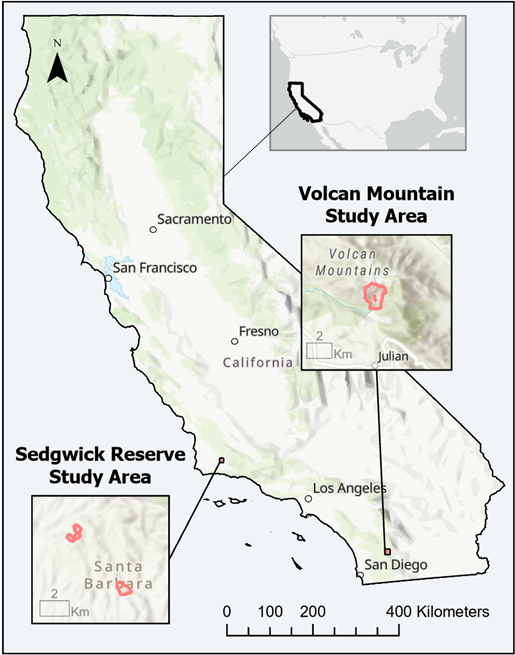
\includegraphics[width=0.75\linewidth]{figures/Overall_Study_Areas_v2.png}
    \caption{\hl{Locations} %MDPI: 1. Some contents are overlapped, please check if they affect reading, if yes, please provide the clearer picture. 2. Please confirm if explanation should be added for the red lines in the image.(MM: The red lines indicate the extent of the UAV LiDAR surveys, which I have added to the caption. The figure is fine as-is.)
 of the Southern California UAV LiDAR surveys—Sedgwick Reserve–Midland School in the Santa Ynez Valley and Volcan Mountain Wilderness Preserve in the Peninsular Range. Red outlines indicate the extent of the UAV LiDAR surveys.}
  \label{fig:overall_study_area}
\end{figure}
\vspace{-9pt}

\begin{figure}[H]
  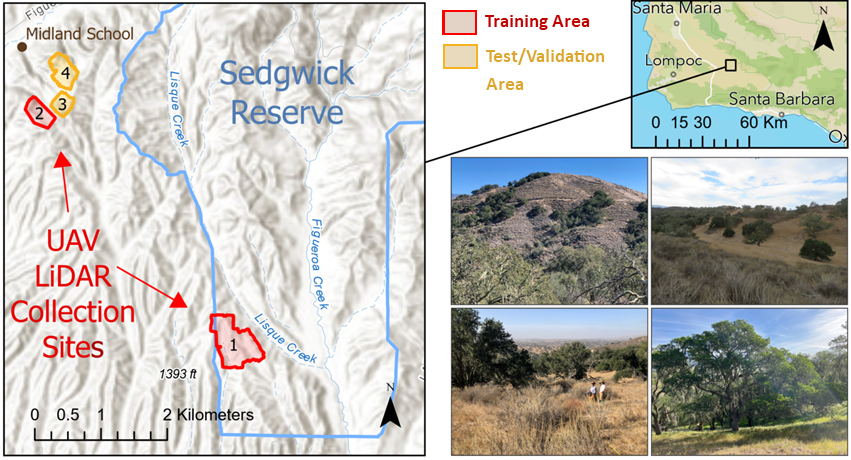
\includegraphics[width=0.95\linewidth]{figures/Sedgwick_Reserve_Study_Area.png}
    \caption{\hl{The} %MDPI: 1. Please confirm whether the incomplete/overlapped/unclear content in this figure affects scientific understanding and if it does, please revise it. 2. Please confirm if explanation should be added for numbers in the image. (MM: The figure is fine as-is. The numbers indicate the UAV LiDAR survey sites in table 1, which I have added to the caption.)
 first study area combines parts of the Sedgwick Reserve and Midland School property in the San Rafael Mountain foothills, Santa Barbara County. It features diverse vegetation, such as oak woodlands, chaparral, grasslands, and coastal sage scrub. Within this area, four UAV LiDAR sites were surveyed, covering a total of 70 hectares. The numbers indicate the UAV LiDAR survey sites which are detailed in Table \ref{tab:lidar_sites}.}
  \label{fig:sedgwick_study_area}
\end{figure}

The area spans elevations from 287 to 852 m and supports a mosaic of vegetation types with varying canopy architectures, including coastal sage scrub, native grasslands, chaparral (shrublands), coast live and blue oak woodlands, valley oak savanna, riparian habitats, and gray pine forests. UAV LiDAR was collected for four sites (totaling about \mbox{71 hectares}) within the study area (Table \ref{tab:lidar_sites}). Given their similar terrain and vegetation, two sites were used for training, while the two smallest were withheld for independent \mbox{model evaluation}.


% % \vspace*{\fill} % push content down from above
% \begin{table}[H]
%   \centering
%   \caption{UAV LiDAR sites used as ground truth for model development}
%   \label{tab:lidar_sites}
%   \begin{tabular}{@{}cllll@{}}
%     \toprule
%     Site & Hectares & Location & Collection Date & Model Use\\ \midrule
%     1 & 38 & Sedgwick Reserve & 30 Jun 2023 & Training\\
%     2 & 12 & Midland School   & 23 Oct 2023 & Training \\
%     3 & 9 & Midland School & 23 Oct 2023 & Test/Validation\\
%     4 & 11 & Midland School   & 28 Sep 2023 & Test/Validation\\

%     5 & 197 & Volcan Mountain & 25 Oct 2024 & \begin{tabular}[c]{@{}l@{}}70\% Training\\ 30\% Test/Validation\end{tabular}\\
%     \bottomrule
%   \end{tabular}
% \end{table}


\begin{table}[H]

  \caption{UAV LiDAR sites used as ground truth for model development.}
  \label{tab:lidar_sites}
  \setlength{\cellWidtha}{\textwidth/5-2\tabcolsep-0.6in}
\setlength{\cellWidthb}{\textwidth/5-2\tabcolsep-0.3in}
\setlength{\cellWidthc}{\textwidth/5-2\tabcolsep+0.3in}
\setlength{\cellWidthd}{\textwidth/5-2\tabcolsep+0.2in}
\setlength{\cellWidthe}{\textwidth/5-2\tabcolsep+0.4in}
\scalebox{1}[1]{\begin{tabularx}{\textwidth}{>{\raggedright\arraybackslash}m{\cellWidtha}>{\raggedright\arraybackslash}m{\cellWidthb}>{\raggedright\arraybackslash}m{\cellWidthc}>{\raggedright\arraybackslash}m{\cellWidthd}>{\raggedright\arraybackslash}m{\cellWidthe}}
    \toprule
    \textbf{Site} & \textbf{Hectares} & \textbf{Location} & \textbf{Collection Date} & \textbf{Model Use} \\ \midrule
    1 & 38  & Sedgwick Reserve & 30 \hl{June} %MDPI: We revised the month format. Please confirm. (MM: confirmed)
 2023 & Training \\
    2 & 12  & Midland School   & 23 \hl{October} 2023 & Training \\
    3 &  9  & Midland School   & 23 \hl{October} 2023 & Test/Validation \\
    4 & 11  & Midland School   & 28 \hl{September} 2023 & Test/Validation \\
    5 & 197 & Volcan Mountain  & 25 \hl{October} 2024 &
        70\% Training\linebreak 30\% Test/Validation \\
    \bottomrule
  \end{tabularx}}
\end{table}


\vspace{-3pt}

% \vspace*{\fill} % push content up from below
The second study area (Figure \ref{fig:volcan_mtn_study_area}) comprises 197 hectares within and adjacent to the Volcan Mountain Wilderness Preserve in the Peninsular Range of Southern California. The reserve is managed by San Diego County and the Volcan Mountain Foundation and ranges in elevation from about 1220 m to over 1675 m.
% \newpage
 It hosts diverse plant communities, including oak woodlands, chaparral, mixed conifer forests, and grasslands. To ensure robust model evaluation across this ecological gradient, roughly 30 percent of the area \mbox{(58 hectares)} was reserved for testing and validation (Table \ref{tab:lidar_sites}). The three holdout zones \mbox{(Figure \ref{fig:volcan_mtn_study_area})} used for model evaluation were selected to reflect the site’s vegetation diversity: the northernmost area includes chaparral that replaced forest following wildfires in 2003 and 2005; the central zone contains dense mixed-conifer and riparian vegetation interspersed with oak woodlands and chaparral; and the southernmost zone is predominantly semi-continuous oak canopy.


\begin{figure}[H]

    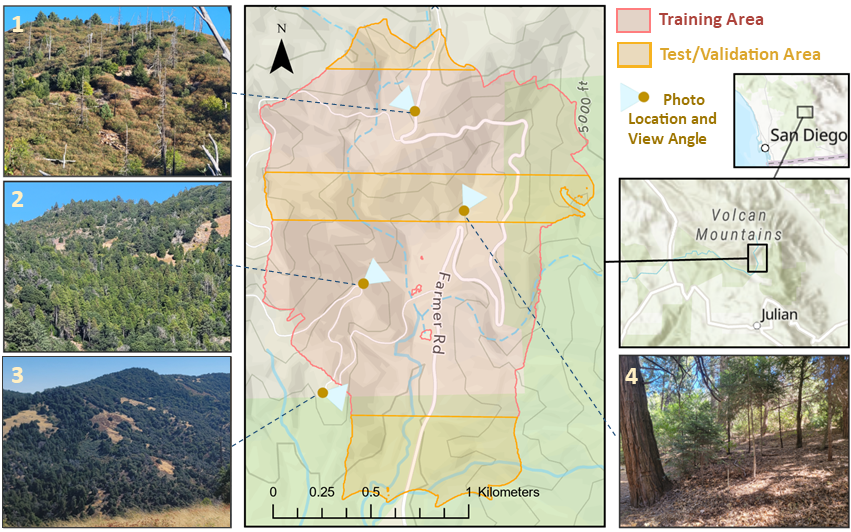
\includegraphics[width=0.98\linewidth]{figures/Volcan_Mtn_Study_Area.png}
    \caption{\hl{Volcan} %MDPI: please add the explanation of the subfigures 1,2,3,4. (MM: added)
 Mountain study area (197 hectares) in the Peninsular Range of Southern California, encompassing diverse vegetation types across an elevation range of 1220 to 1675 m. Thirty percent of the site (58 hectares) was set aside for testing/validation in three zones: post-fire chaparral in the north, mixed conifer and riparian vegetation with oak and chaparral in the center, and oak woodland with semi-continuous canopy in the south. Subfigures 1,2,3,4 show photos of the different vegetation types in the study area.}
    \label{fig:volcan_mtn_study_area}
\end{figure}






\subsection{The Data}

All remote‐sensing assets were co-registered within a common tiling framework covering both study sites.   First, the UAV‐LiDAR acquisition footprints were tessellated into 10 m × 10 m analysis tiles with 15\% overlap, yielding an initial set of 9800 tiles at Sedgwick–Midland and 26,557 tiles at Volcan Mountain. Each tile served as the spatial key for assembly of a four-layer data stack (Table \ref{tab:data_summary}).

% \begin{enumerate}[leftmargin=*]
%     \item \textbf{UAV LiDAR} point clouds (\textit{Sedgwick}-2023, 300 pts/m\textsuperscript{2}; \textit{Volcan}–2024, 300 pts/m\textsuperscript{2})
%     \item \textbf{3DEP airborne LiDAR} (\textit{Sedgwick}-2018, 22 pts/m\textsuperscript{2}; \textit{Volcan}-2015–16, 6 pts/m\textsuperscript{2})
%     \item \textbf{UAVSAR radar} coverage from 2014 to 2024 (6.17 m GSD)
%     \item \textbf{NAIP imagery} coverage from 2014 to 2022 (0.6–1 m GSD)
% \end{enumerate}

\begin{table}[H] % Using [H] from the float package to place it here.
\tablesize{\footnotesize}
\caption{\hl{Summary} %MDPI: 1. Please add the explanation of “N/A”. 2. Please confirm the alignment change. (MM: added explanation of N/A in footnote; alignment change is fine)
 of remote sensing datasets used in the data stack.}
\label{tab:data_summary}
\setlength{\cellWidtha}{\textwidth/4-2\tabcolsep+0.1in}
\setlength{\cellWidthb}{\textwidth/4-2\tabcolsep-0.1in}
\setlength{\cellWidthc}{\textwidth/4-2\tabcolsep+0.4in}
\setlength{\cellWidthd}{\textwidth/4-2\tabcolsep-0.4in}
\scalebox{1}[1]{\begin{tabularx}{\textwidth}{>{\raggedright\arraybackslash}m{\cellWidtha}>{\raggedright\arraybackslash}m{\cellWidthb}>{\raggedright\arraybackslash}m{\cellWidthc}>{\raggedright\arraybackslash}m{\cellWidthd}}
\toprule
\textbf{Data Source} & \textbf{Role in Study} & \textbf{Details} & \textbf{Revisit Rate} \\
\midrule
UAV LiDAR & Reference Data & $>$300 pts/m\textsuperscript{2} \newline \textit{\hl{Acquired: 2023--2024} %MDPI: Please confirm if the italics are necessary; if not, please remove them. The following highlights are the same. (MM: confirmed)
} & N/A\textsuperscript{1} \\
\addlinespace
3DEP Airborne LiDAR & Sparse Input & Sedgwick: $\sim$22 pts/m\textsuperscript{2} (2018) \newline Volcan: $\sim$6 pts/m\textsuperscript{2} (2015–\hl{2016}%MDPI: We changed it to “2016”, please confirm (MM: confirmed)
) & N/A\textsuperscript{1} \\
\addlinespace
UAVSAR (L-band) & Ancillary Input & 6.17 m GSD \newline \textit{\hl{Coverage: 2014--2024}} & $\sim$2--3 years \\
\addlinespace
NAIP (Optical) & Ancillary Input & 0.6–1 m GSD \newline \textit{\hl{Coverage: 2014--2022}} & $\sim$2 years \\
\bottomrule
\end{tabularx}}
\noindent{\footnotesize{\textsuperscript{1} Single acquisition; no revisit.}}
\end{table}


\vspace{-3pt}

By standardizing on overlapping 10 m patches, we guarantee that each training example draws from the same footprint across sensors—ensuring the model learns consistent, co-registered features from LiDAR, SAR, and imagery.

\subsubsection{UAV LiDAR Data}
\textit{\hl{Sedgwick and Midland Sites}%MDPI: Please confirm if the italics are necessary; if not, please remove them. The following highlights are the same. (MM: confirmed)
}---Between June and October 2023, UAV LiDAR data were collected by San Diego State Geography Department staff on the Sedgwick and Midland School Sites using a DJI Matrice 300 drone (DJI, Shenzhen, China) %MDPI: Please state the name of the manufacturer, city, and country from where the equipment was sourced. Please check the whole paper and add the information for all the equipment that used for this paper.(MM: added)
 equipped with a TrueView 515 LiDAR instrument (GeoCue, Madison, AL, USA)/%MDPI: Please state the name of the manufacturer, city, and country from where the equipment was sourced. (MM: added)
The drone was flown at an altitude of approximately 60 m above ground level, achieving a point density of around 300 points per square meter.

\textit{\hl{Volcan Mountain Site}}---On \hl{25 October 2024}%MDPI: We revised the date format. Please confirm.(MM: confirmed)
, the same Geography Department staff conducted flights using a DJI Matrice 350 drone (DJI, Shenzhen, China) equipped with a TrueView 540 LIDAR system (GeoCue, Madison, AL, USA). This newer drone and sensor were flown at a higher altitude of approximately \mbox{110 m} above ground level and still achieved a point density of over 600 points per \mbox{square meter}.

\subsubsection{Crewed Airborne LiDAR}
The available crewed airborne LiDAR (C-ALS) data includes two separate 3DEP datasets. The Sedgwick 3DEP dataset, collected in 2018, has a point density of 22 pts/m\textsuperscript{2}. The C-ALS data for the Volcan Mountain site was collected between October 2015 and November 2016 and has a point density of 6.3 pts/m\textsuperscript{2} \citep{usgs_usgs_2016}. Both datasets were obtained from Microsoft's Planetary Computer \citep{us_geological_survey_3d_elevation_program_usgs_2023,planetary_computer}.
In addition to the point X, Y, and Z values we include three per-return attributes—intensity (16-bit integer 0–65,535 pulse magnitude), return number (ordinal of the return within its pulse), and number of returns (total returns from that pulse)—each standardized using the global mean and standard deviation computed across the full 3DEP dataset.


\subsubsection{Synthetic Aperture Radar (SAR)}
Fully polarimetric L-band imagery (23.84 cm wavelength) from NASA’s UAVSAR system was obtained with the Alaska Satellite Facility’s \texttt{asf\_search} (version 8.1.1) Python %MDPI: Please state which version of the software was used. (MM: added)
 API \citep{alaska_search}. The UAVSAR flights were conducted from a Gulfstream-III platform with bidirectional acquisitions from opposite look directions at an average altitude of 12,495 m, providing multi-perspective radar coverage of the landscape at 6.17 m ground resolution. We utilized six fully polarimetric multi-look cross-product channels: \texttt{HHHH}, \texttt{HVHV}, \texttt{VVVV}, \texttt{HHHV}, \texttt{HHVV}, and \texttt{HVVV}. The specific campaigns and acquisition details for each study site are summarized in Table \ref{tab:imagery_timeline_v2}. For every \SI{10}{m} × \SI{10}{m} 3DEP tile, we extracted a co-centered \SI{20}{m} × \SI{20}{m} UAVSAR chip to accommodate layover and shadow extent, then bilinearly resampled each chip to \SI{5}{m} GSD before fusion with NAIP imagery and LiDAR.


\begin{table}[H]
\tablesize{\small}
\caption{\hl{Timeline} %MDPI: We revised the lines format in the table. Please confirm. (MM: confirmed)
 of NAIP and UAVSAR acquisitions for both study sites.}
\label{tab:imagery_timeline_v2}

\setlength{\cellWidtha}{\textwidth/5-2\tabcolsep-0.4in}
\setlength{\cellWidthb}{\textwidth/5-2\tabcolsep-0in}
\setlength{\cellWidthc}{\textwidth/5-2\tabcolsep+0.2in}
\setlength{\cellWidthd}{\textwidth/5-2\tabcolsep-0in}
\setlength{\cellWidthe}{\textwidth/5-2\tabcolsep+0.2in}
\scalebox{1}[1]{\begin{tabularx}{\textwidth}{>{\centering\arraybackslash}m{\cellWidtha}>{\centering\arraybackslash}m{\cellWidthb}>{\centering\arraybackslash}m{\cellWidthc}>{\centering\arraybackslash}m{\cellWidthd}>{\centering\arraybackslash}m{\cellWidthe}}
\toprule
& \multicolumn{2}{c}{\textbf{Volcan Mountain}} & \multicolumn{2}{c}{\textbf{Sedgwick Reserve}} \\
\midrule
\textbf{Year} & \textbf{NAIP (GSD)} & \textbf{UAVSAR (\# Looks\textsuperscript{1})} %MDPI: please add the explanation of “#” (MM: added in footnote)
 & \textbf{NAIP (GSD)} & \textbf{UAVSAR (\# Looks\textsuperscript{1})} \\
\midrule
2014 & May (1 m) & \hl{June} %MDPI: We revised the month format in the whole table. Please confirm this revision. (MM: confirmed)
 (3), October (2) & June (1 m) & June (8) \\
\addlinespace
2016 & April (60 cm) & --- & June (60 cm) & April (6) \\
\addlinespace
2018 & August (60 cm) & October (2) & July (60 cm) & --- \\
\addlinespace
2020 & April (60 cm) & --- & May (60 cm) & --- \\
\addlinespace
2021 & --- & November (2) & --- & --- \\
\addlinespace
2022 & April (60 cm) & --- & May (60 cm) & --- \\
\addlinespace
2023 & --- & --- & --- & September (6)\textsuperscript{2} \\
\addlinespace
2024 & --- & --- & --- & October (2) \\
\bottomrule
\end{tabularx}}
\noindent{\footnotesize
\textsuperscript{1} The count of UAVSAR acquisition passes that month. Each listed month includes at least two opposing look directions; counts >2 indicate additional passes that may be distinct or repeated look geometries.\\
\textsuperscript{2} Part of the NASA FireSense initiative.
}
\end{table}


\subsubsection{High-Resolution Aerial Imagery}
We ingested NAIP imagery through the Microsoft Planetary Computer STAC API \citep{planetary_computer} for survey years 2014–2022. NAIP provides four-band (red, green, blue, and near-infrared) orthoimagery of the conterminous United States, collected at peak green-up on a two- to three-year cycle. Prior to the 2016 flight season, data were delivered at 1 m ground-sample distance (GSD); since 2016, the native resolution has been 60 cm. A complete timeline of these acquisitions and their resolutions is provided in Table \ref{tab:imagery_timeline_v2}. For every 10 m × 10 m 3DEP tile, we extracted a 20 m × 20 m NAIP chip centered on the same point to accommodate viewing-geometry variance and to capture neighboring shadows. All NAIP scenes were then resampled to a common 50 cm grid.



\subsection{Data Cleaning and Preprocessing}
To reduce computational load and give the upsampling network a uniform-density target, we downsampled the UAV LiDAR for every tile with an adaptive anisotropic voxel grid. Each cloud was first voxelized at a 4 cm × 4 cm × 2 cm resolution; if more than 50,000 points remained, the horizontal voxel edge was incrementally enlarged (keeping the vertical edge at 50\% of that value), and the filter was reapplied until the count fell below the limit%EE: Please check intended meaning has been retained (MM: confirmed)
. The resulting point sets preserve fine vertical structure while standardizing horizontal density.

To bound memory use and keep attention context sizes tractable, we cap the input 3DEP point cloud at $N_{\max}=10{,}000$ points per $10\times10$\,m tile. If a tile exceeds this count, we randomly subsample to $N_{\max}$ points; fewer than 1\% of tiles were affected. This cap defines the maximum attention sequence length and thus the model's memory footprint.

The dataset was partitioned into training, validation, and test sets using reference polygons to ensure the holdout sets captured the full environmental gradients found in the training data. During supervised training/evaluation, we applied quality thresholds—UAV to 3DEP point count ratio > 2 and at least 16,000 UAV LiDAR points and 200 3DEP points per tile—to exclude edge-of-flight tiles and extremely sparse cases, ensuring a meaningfully denser UAV reference and minimally informative 3DEP input for stable supervision. These thresholds served only as dataset curation filters and are not required at inference.

\subsection{Data Augmentation}
To increase the model's robustness and prevent overfitting, we expanded the training dataset from 24,000 to 40,000 tiles via data augmentation \cite{zhu2024advancements, shorten2019survey}. First, we preferentially selected source tiles for this process, prioritizing those with high structural complexity (z-variance) and large vegetation changes. Each selected source tile was then used to generate a new, augmented sample by applying a random combination of transformations. These included geometric operations (rotations and reflections) applied to all data layers and point cloud-specific perturbations (random point removal and jittering) applied only to the input LiDAR data.


%%%%%%%%%%%%%%%%%%%%%%%%%%%%%%%%%%%%%%%%%%
\subsection{Model Architecture}
\label{sec:architecture}
\textls[-15]{Our multi-modal upsampling framework transforms a sparse 3DEP point cloud, plus co-registered NAIP and UAVSAR image chips, into a denser 3D point cloud (Figure~\ref{fig:pipeline}). The network is built around the \textit{\hl{Local–Global Point Attention Block} %MDPI: Please confirm if the bold formatting is necessary; if not, please remove it. (MM: converted to italics instead of bold)
} (LG-PAB; \hl{Section} %MDPI: We revised the symbol into ``Section'' for section citation. Please confirm this revision. (MM: Confirmed)
 \ref{sec:lgpab}),} which provides permutation‐invariant feature learning, optional feature-guided upsampling, and long-range geometric context. Five macro components are arranged in a feed-forward sequence: (1) point feature extraction, (2) imagery encoding, (3) cross-attention fusion, (4)~feature expansion and refinement, and (5) point decoding.






\paragraph{Notation Conventions}
Throughout this section, we use the following notations for tensor dimensions:
\begin{itemize}
    \item Counts: $N_{\text{pts}}$ (number of input points), $N_{\text{curr\_pts}}$ (current points in LG-PAB), \mbox{$N_{\text{pts\_up}} = R_{\text{up}} \cdot N_{\text{pts}}$} (upsampled points), $N_{\text{patch}}$ (number of image patches, default 16), $N_{\text{time}}$ (temporal stack length), and $N_{\text{looks}}$ (maximum look angles, $\leq$2);
    \item Dimensions: $D_{\text{coord}} = 3$ (coordinate dimension), $D_{\text{attr}}$ (attribute dimension), \mbox{$D_{\text{p\_feat}} = 256$ (point feature dimension), $D_{\text{p\_in}}$} (input point feature dimension), $D_{\text{p\_out}}$ (output point feature dimension), and $D_{\text{token}} = 128$ (token dimension);
    \item Channels: $C_{\text{naip}} = 4$ (NAIP channels), and $C_{\text{uavsar}} = 6$ (UAVSAR channels);
    \item Image dimensions: $H_{\text{naip}} = W_{\text{naip}} = 40$ (NAIP height/width), $H_{\text{uavsar\_pr}} = W_{\text{uavsar\_pr}} = 4$ (UAVSAR patch region height/width).
    \item Other: $R_{\text{up}}$ (upsampling ratio, default 2), $k_{\text{knn}} = 16$ (k-nearest neighbors).
\end{itemize}
For tensors, we use the notation TensorSymbol: (dim$_1$, dim$_2$, ..., dim$_k$) to describe their dimensions.

\noindent\textit{Figure notation bridge.} In Fig.~\ref{fig:lgpab} the generic diagram labels \texttt{in\_features} and \texttt{out\_features} (and the shortened \texttt{out\_feat} on two arrows) correspond to $D_{\text{p\_in}}$ and $D_{\text{p\_out}}$ in the above notation. (We used Mermaid for the schematic, which does not support mathematical subscripts, so plain text placeholders were used.)


\begin{figure}[H]
\begin{adjustwidth}{-\extralength}{0cm}
    \centering
    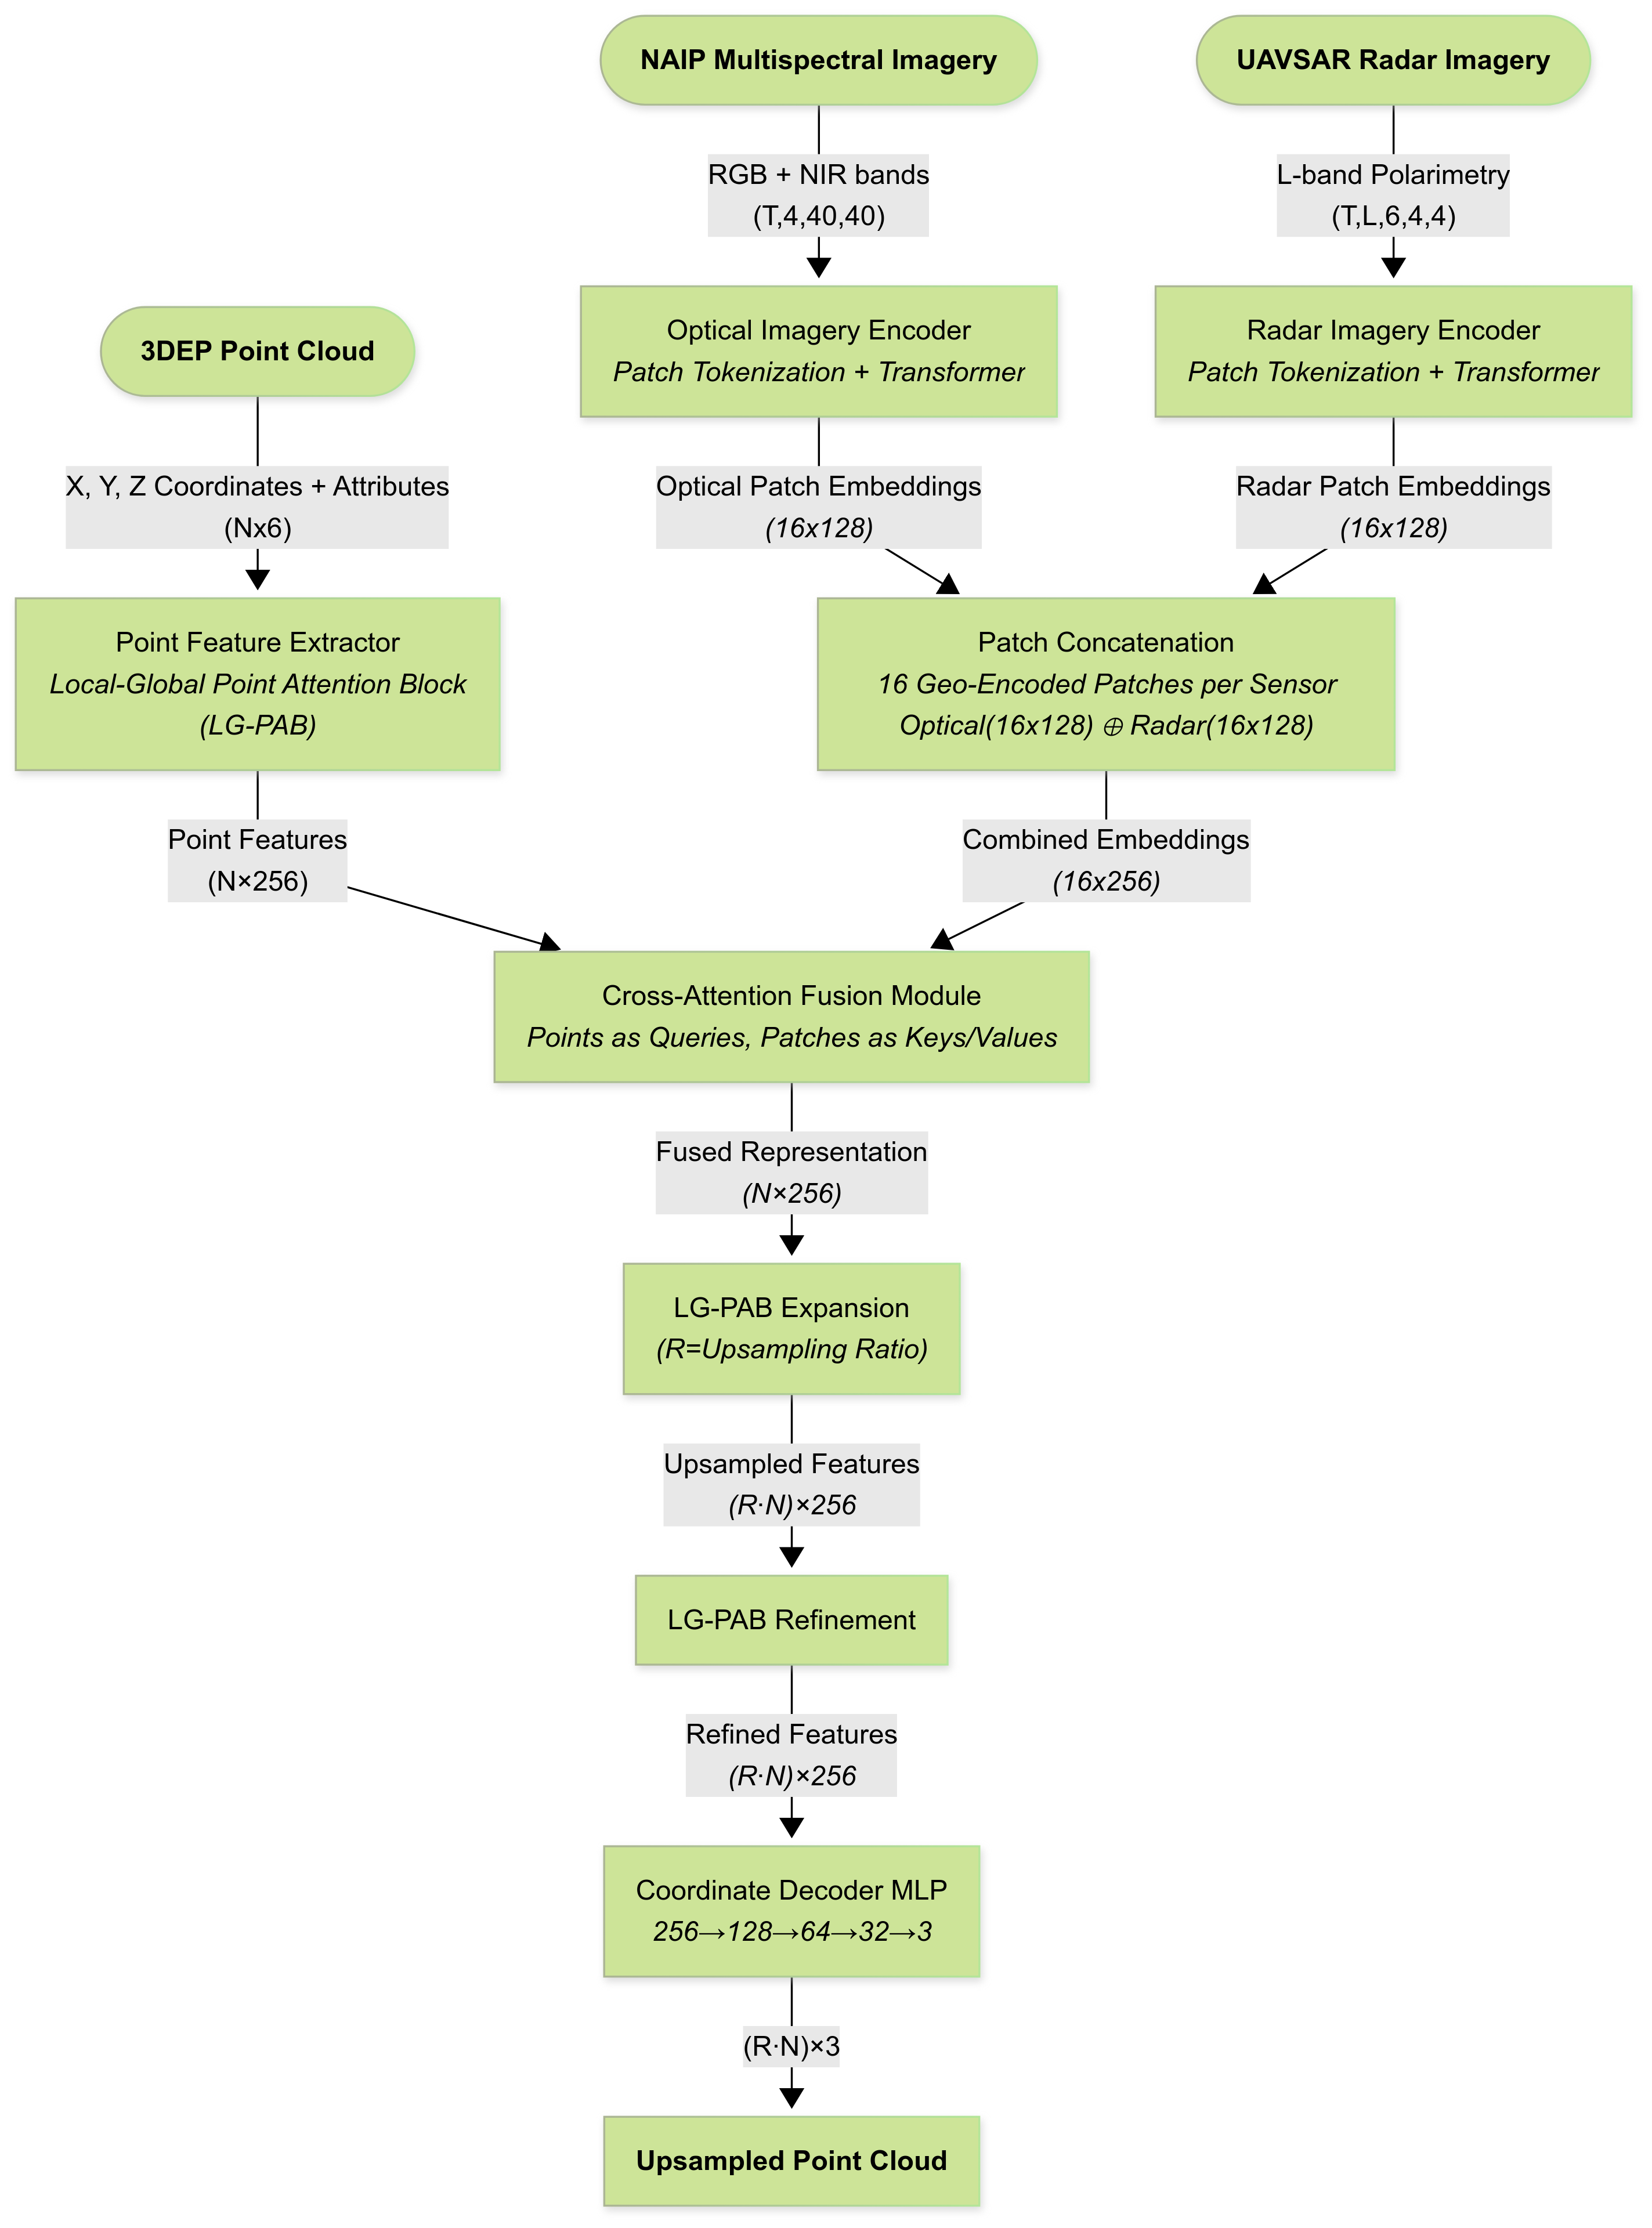
\includegraphics[trim=0mm 0mm 0mm 9mm, clip, width=0.9\linewidth]{figures/Overall_Architecture.png}
    \end{adjustwidth}
    \caption{\hl{The} %MDPI: To reduce the blank page, we moved Figure 5 here. Please confirm.
 overall multi-modal upsampling architecture. Key components include local–global point attention blocks, modality-specific imagery encoders for the processing of optical (NAIP) and radar (UAVSAR) data, and a cross-attention fusion module for combining imagery and LiDAR features.}
    \label{fig:pipeline}
\end{figure}


Given an input cloud ($P_{\text{in}}: (N_{\text{pts}}, D_{\text{coord}})$) with \hl{points} %MDPI: %MDPI: 1. Please check if all bold format should be retained in equations in the whole paper. 2.Please ensure all variables/values in the equation appear in the same format in the text (normal/italic/bold/subscript/superscript). (MM: confirmed)
 ($\{\mathbf{{x}}_i\}_{i=1}^{N_{\text{pts}}}\subset\mathbb{R}^{D_{\text{coord}}}$) and attributes ($\mathbf{a}_i: (D_{\text{attr}})$), the network outputs $P_{\text{out}}: (N_{\text{pts\_up}}, D_{\text{coord}})$ with points $\{\hat{\mathbf{x}}_j\}_{j=1}^{N_{\text{pts\_up}}}$, where $N_{\text{pts\_up}} = R_{\text{up}} \cdot N_{\text{pts}}$ (typically $R_{\text{up}} = 2$).

An overview is presented as follows:

\begin{enumerate}[leftmargin=*]
\item \textbf{\hl{LG-PAB Extractor} %MDPI: Please confirm if the bold formatting is necessary; if not, please remove it. The following highlights are the same.(MM: confirmed)
} $\;\mathcal{E}_{\mathrm{pt}}$
      $\;\rightarrow$ local–global point features $F: (N_{\text{pts}}, D_{\text{p\_feat}})$;
\item \textbf{\hl{Imagery Encoders}} $\;\mathcal{E}_{\mathrm{opt}},\mathcal{E}_{\mathrm{rad}}$
      $\;\rightarrow$ NAIP and UAVSAR patch embeddings $E_{\text{opt}}, E_{\text{rad}}: (N_{\text{patch}}, D_{\text{token}})$;
\item \textbf{\hl{Cross-Attention Fusion}} $\;\mathcal{F}_{\mathrm{ca}}$
      $\;\rightarrow$ enriched point features $F_{\!\mathrm{fused}}: (N_{\text{pts}}, D_{\text{p\_feat}})$;
\item \textbf{\hl{LG-PAB Expansion \& Refinement}}
      $\;\rightarrow$ upsampled features $F^{\uparrow}: (N_{\text{pts\_up}}, D_{\text{p\_feat}})$ and coordinates $P^{\uparrow}: (N_{\text{pts\_up}}, D_{\text{coord}})$;
\item \textbf{\hl{MLP Decoder}} $\;\rightarrow$ residual offsets $\Delta P: (N_{\text{pts\_up}}, D_{\text{coord}})$ and final coordinates $P_{\mathrm{out}}: (N_{\text{pts\_up}}, D_{\text{coord}})$.
\end{enumerate}


\paragraph{Complexity, memory, and sequence length across stages.}
Global multi-head attention remains quadratic in the number of points within a tile. The 10\,m tiling and the input cap $N_{\max}=10{,}000$ fix the extractor’s attention sequence length; with the feature-guided expansion set to $R_{\text{up}}=2$, the largest sequence arises immediately after expansion and is at most $\approx 2\times N_{\text{pts}} \le 20{,}000$ before refinement and decoding. We implement global attention with FlashAttention, which reduces memory traffic while preserving exact attention. Under these bounds, we observed stable runtime and memory without requiring additional approximations or pruning.

% --- LG-PAB (its own page) ---------------------------------------------------
% \clearpage
\subsection{The Local–Global Point Attention Block (LG-PAB)}
\label{sec:lgpab}

% \begin{wrapfigure}[40]{r}{0.43\textwidth}

% \end{wrapfigure}%

Figure~\ref{fig:lgpab} presents a flow chart of the \emph{\hl{Local–Global Point Attention Block}%MDPI: Please confirm if the italics are necessary; if not, please remove them. The following highlights are the same.
}, the fundamental unit used three times in our architecture (extraction, expansion, and refinement stages). Each LG-PAB converts an input tuple $\langle X, P \rangle$ consisting of point features ($X: (N_{\text{curr\_pts}}, D_{\text{p\_in}})$) and 3D coordinates ($P: (N_{\text{curr\_pts}}, D_{\text{coord}})$) into refined (and optionally upsampled) features and positions. The block proceeds through the following stages that appear in the diagram:

\begin{enumerate}[leftmargin=*]
\item \textbf{\hl{Local Attention Block:}}
      A %EE: Attention AE.
      \textsc{multi-head point Transformer} operates on a $k_{\text{knn}}$-nearest-neighbor graph ($k_{\text{knn}}\,{=}\,16$) to capture fine-scale geometry. Its output passes through a two-layer \textsc{Feed-Forward Network} (FFN) with GELU activation, producing an intermediate tensor
      ($Z: (N_{\text{curr\_pts}}, R_{\text{up}} \cdot D_{\text{p\_out}})$). When the upsampling ratio is $R_{\text{up}}\,{=}\,1$, this step already delivers the final per-point features.

\item[\emph{2\,a}] \textbf{\hl{Feature-Guided Upsampling (optional):} %MDPI: 1. Please confirm if the bold are necessary; if not, please remove them. 2. Please check if the list label is right and if the italics format can be removed for it. (MM: Confirmed. Keep as-is)
}
      If $R_{\text{up}}\,{>}\,1$ (expansion stage), the intermediate tensor is reshaped to $[N_{\text{curr\_pts}}, R_{\text{up}}, D_{\text{p\_out}}]$, effectively cloning each feature vector $R_{\text{up}}$ times.
      A small position-generator MLP then predicts a 3D offset for every clone, yielding new coordinates
      ($\hat{P} = P^{\text{rep}} + \Delta P: (N_{\text{curr\_pts}} \cdot R_{\text{up}}, D_{\text{coord}})$).
      The features are flattened back to $[N_{\text{curr\_pts}} \cdot R_{\text{up}}, D_{\text{p\_out}}]$.

\item \textbf{\hl{Global Attention Block}:}
      To impose long-range coherence, the upsampled (or original) features are processed by %EE: Attention AE.
      \textsc{Position-Aware Global Flash Attention}. Coordinates are first embedded by a two-layer MLP, concatenated to the features, and fed to a four-head FlashAttention layer that attends across \emph{\hl{all}} points in the tile. A second FFN refines the attended features, after which residual connections and LayerNorm complete the block.
\end{enumerate}



% --- Imagery Encoders (its own page) ----------------------------------------
% \clearpage
\subsection{Imagery Encoders}
\label{sec:img_enc}

% \begin{wrapfigure}[20]{r}{0.45\textwidth}
%   \vspace{-25pt}
%   \centering
%   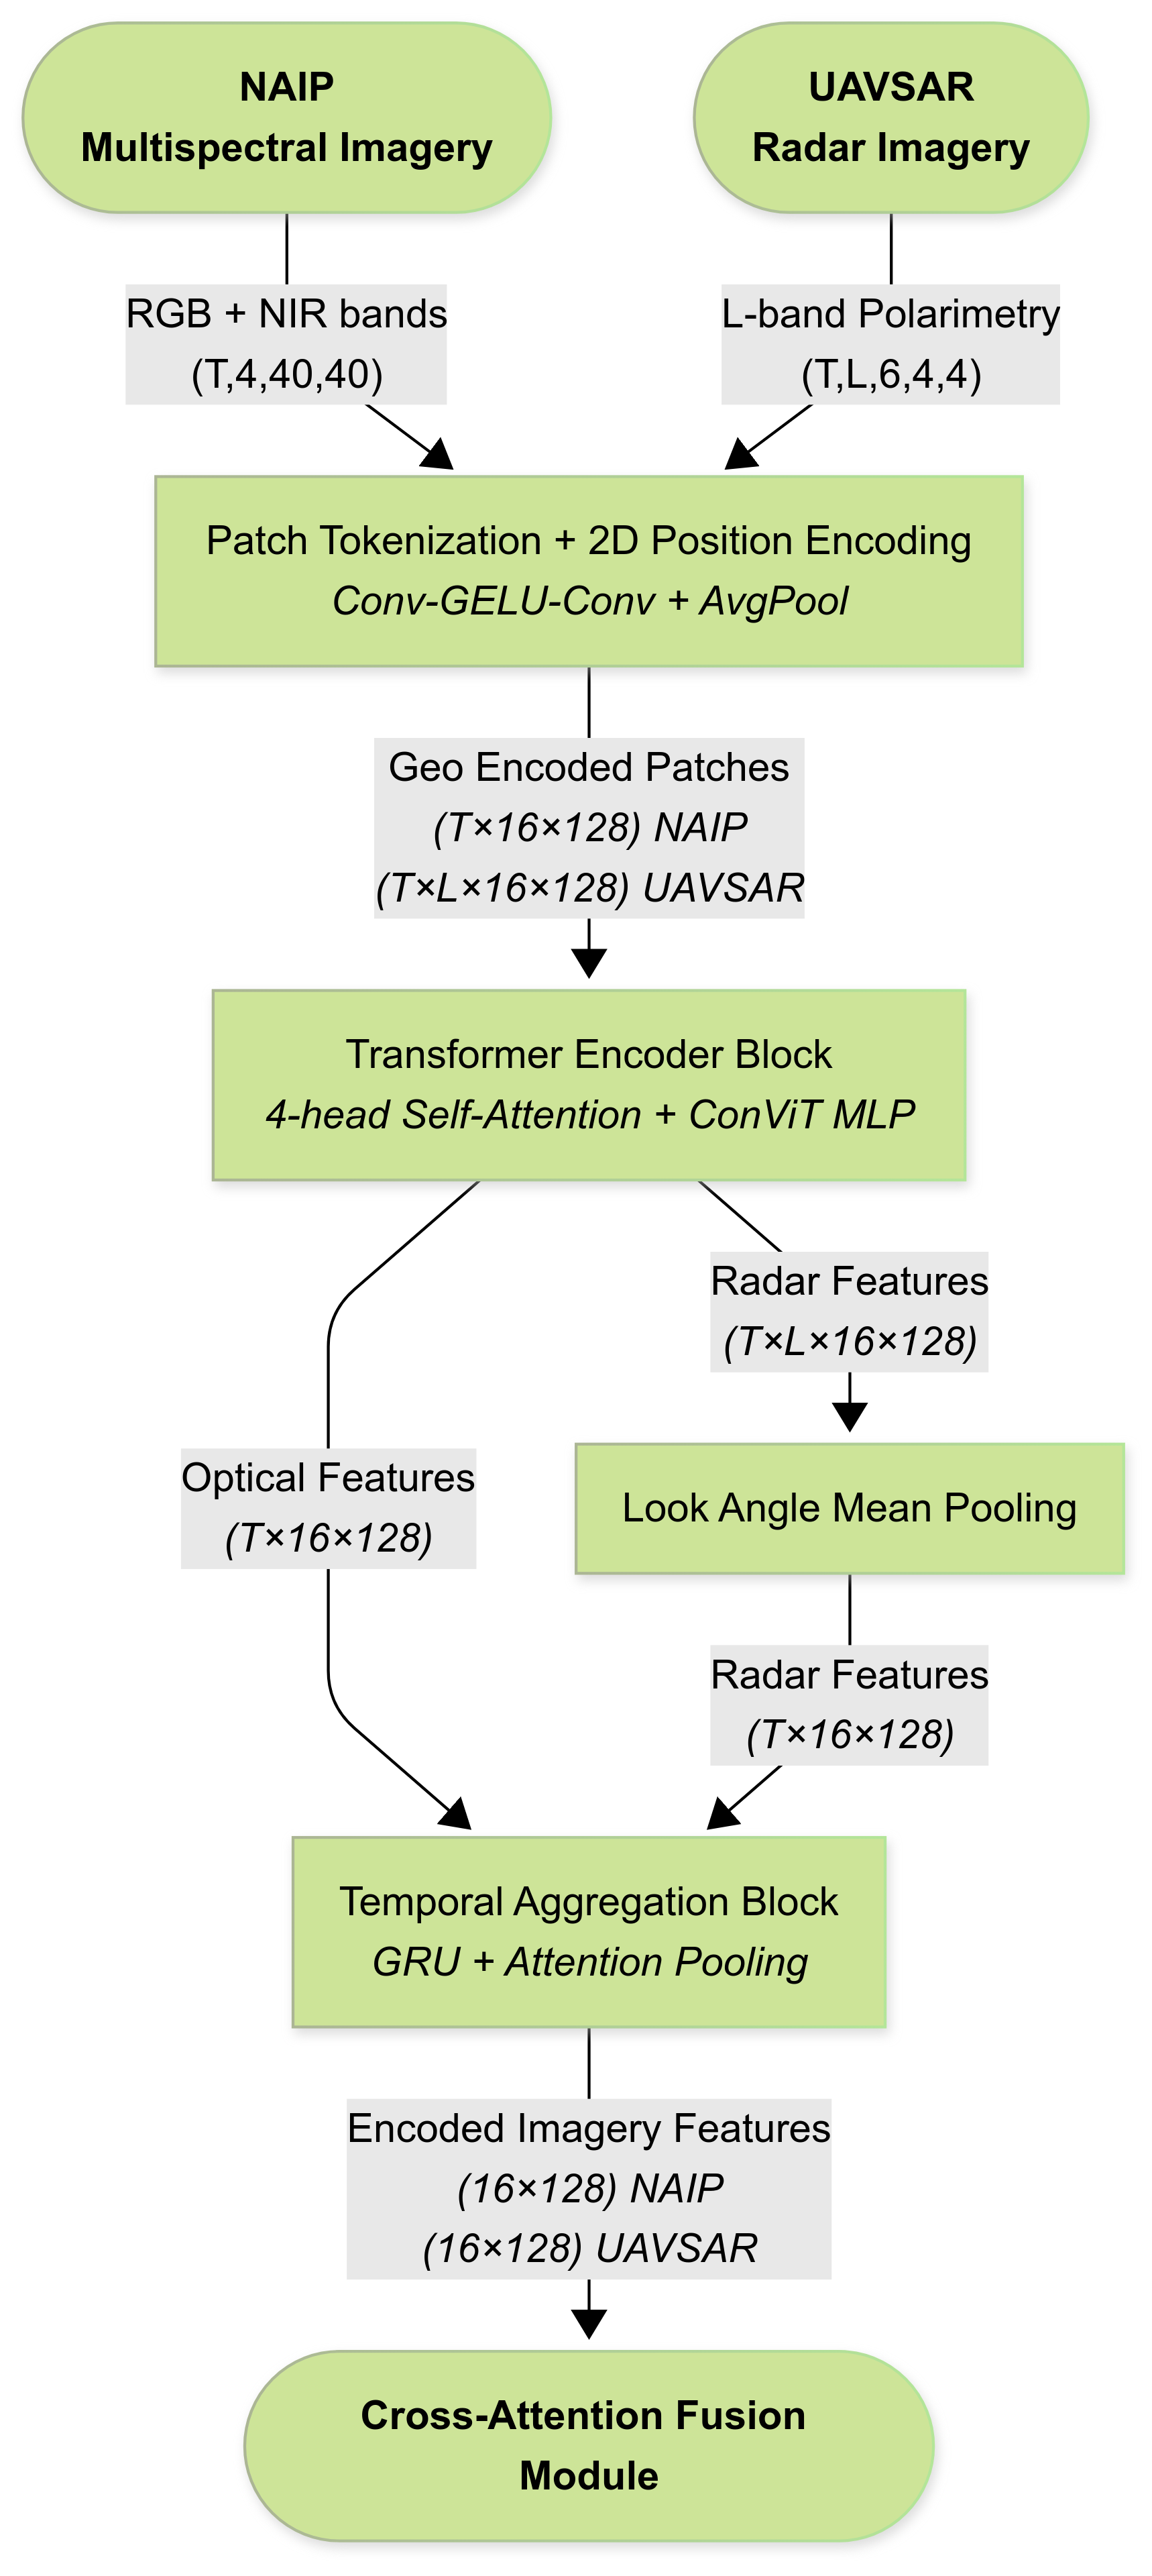
\includegraphics[trim=0mm 0mm 20mm 0mm, clip, width=0.43\textwidth]{figures/Imagery_Encoders.png}
%   \caption{Architecture diagram of the imagery encoders. Image stacks from NAIP (optical) and UAVSAR (radar) pass sequentially through Patch Tokenization, Transformer Encoder blocks for spatial context modeling, and a Temporal GRU-Attention Head for temporal aggregation.}
%   \label{fig:imgenc}
% \end{wrapfigure}%


Optical (NAIP) and radar (UAVSAR) image chips are processed by a \emph{\hl{shared five-stage encoder}} (with modality-specific weights) that converts each image stack into a fixed set of patch tokens. The encoder stages—illustrated in Figure~\ref{fig:imgenc}—are outlined as follows:

\begin{enumerate}[leftmargin=*]
\item \textbf{\hl{Patch Tokenization:}}
      A two-layer Conv–GELU–Conv stem with a stride of 1 %EE: Please check intended meaning has been retained (MM: confirmed)
      followed by average pooling (stride=$\texttt{patch\_size}$) extracts features on a $4\times4$ grid. This design mirrors shifted patch tokenization, which adds local texture bias to Vision Transformers (ViTs) and improves sample efficiency on small datasets \cite{lee2021vision}.
 (Conv1: $C_{in}\rightarrow D_{\text{token}}/2$, $3\times3$, stride 1, pad 1; Conv2: $D_{\text{token}}/2\rightarrow D_{\text{token}}$, $3\times3$, stride 1, pad 1; AvgPool: kernel=stride=$\texttt{patch\_size}=10$.) The \mbox{$N_{\text{patch}}=16$ patches} are flattened to $Z_{\text{tok}}: (N_{\text{patch}}, D_{\text{token}})$ and normalized via LayerNorm.


\item \textbf{\hl{2D Positional Encoding:}}
      Normalized patch centers are embedded via a two-layer MLP and added to the tokens: $Z_{\text{pos}} = Z_{\text{tok}} + \text{MLP}_{\text{pos}}(x,y)$.

\item \textbf{\hl{Transformer Encoder Block.}}
      A 4-head self-attention layer is paired with LayerScale ($\gamma \approx 10^{-5}$), a learnable scalar that stabilizes deep Transformers \cite{touvron2021going}. The accompanying MLP includes a depth-wise 1D convolution, following the ConViT approach to introduce a soft convolutional inductive bias \cite{dascoli2021convit}. MLP: $D_{\text{token}} \rightarrow 4 D_{\text{token}}$ (depth-wise 1-D conv $k=3$) $\rightarrow D_{\text{token}}$. The block outputs $Z_{\text{enc}}: (N_{\text{patch}}, D_{\text{token}})$.



\item \textbf{\hl{Temporal GRU–Attention Head.}}
      For inputs with a temporal length of $N_{\text{time}}$, a bidirectional Gated Recurrent Unit (GRU) with attention pooling aggregates tokens into patch descriptors ($E_{\text{patch}}: (N_{\text{patch}}, D_{\text{token}})$).
\end{enumerate}

Full per-component layer specifications (including fusion projections, LG-PAB FFNs, upsampling position generator, and coordinate decoder) appear in Appendix Table~\ref{tab:layer_specs} for transparency and reproducibility.

\vspace{-9pt}

\begin{figure}[H]

  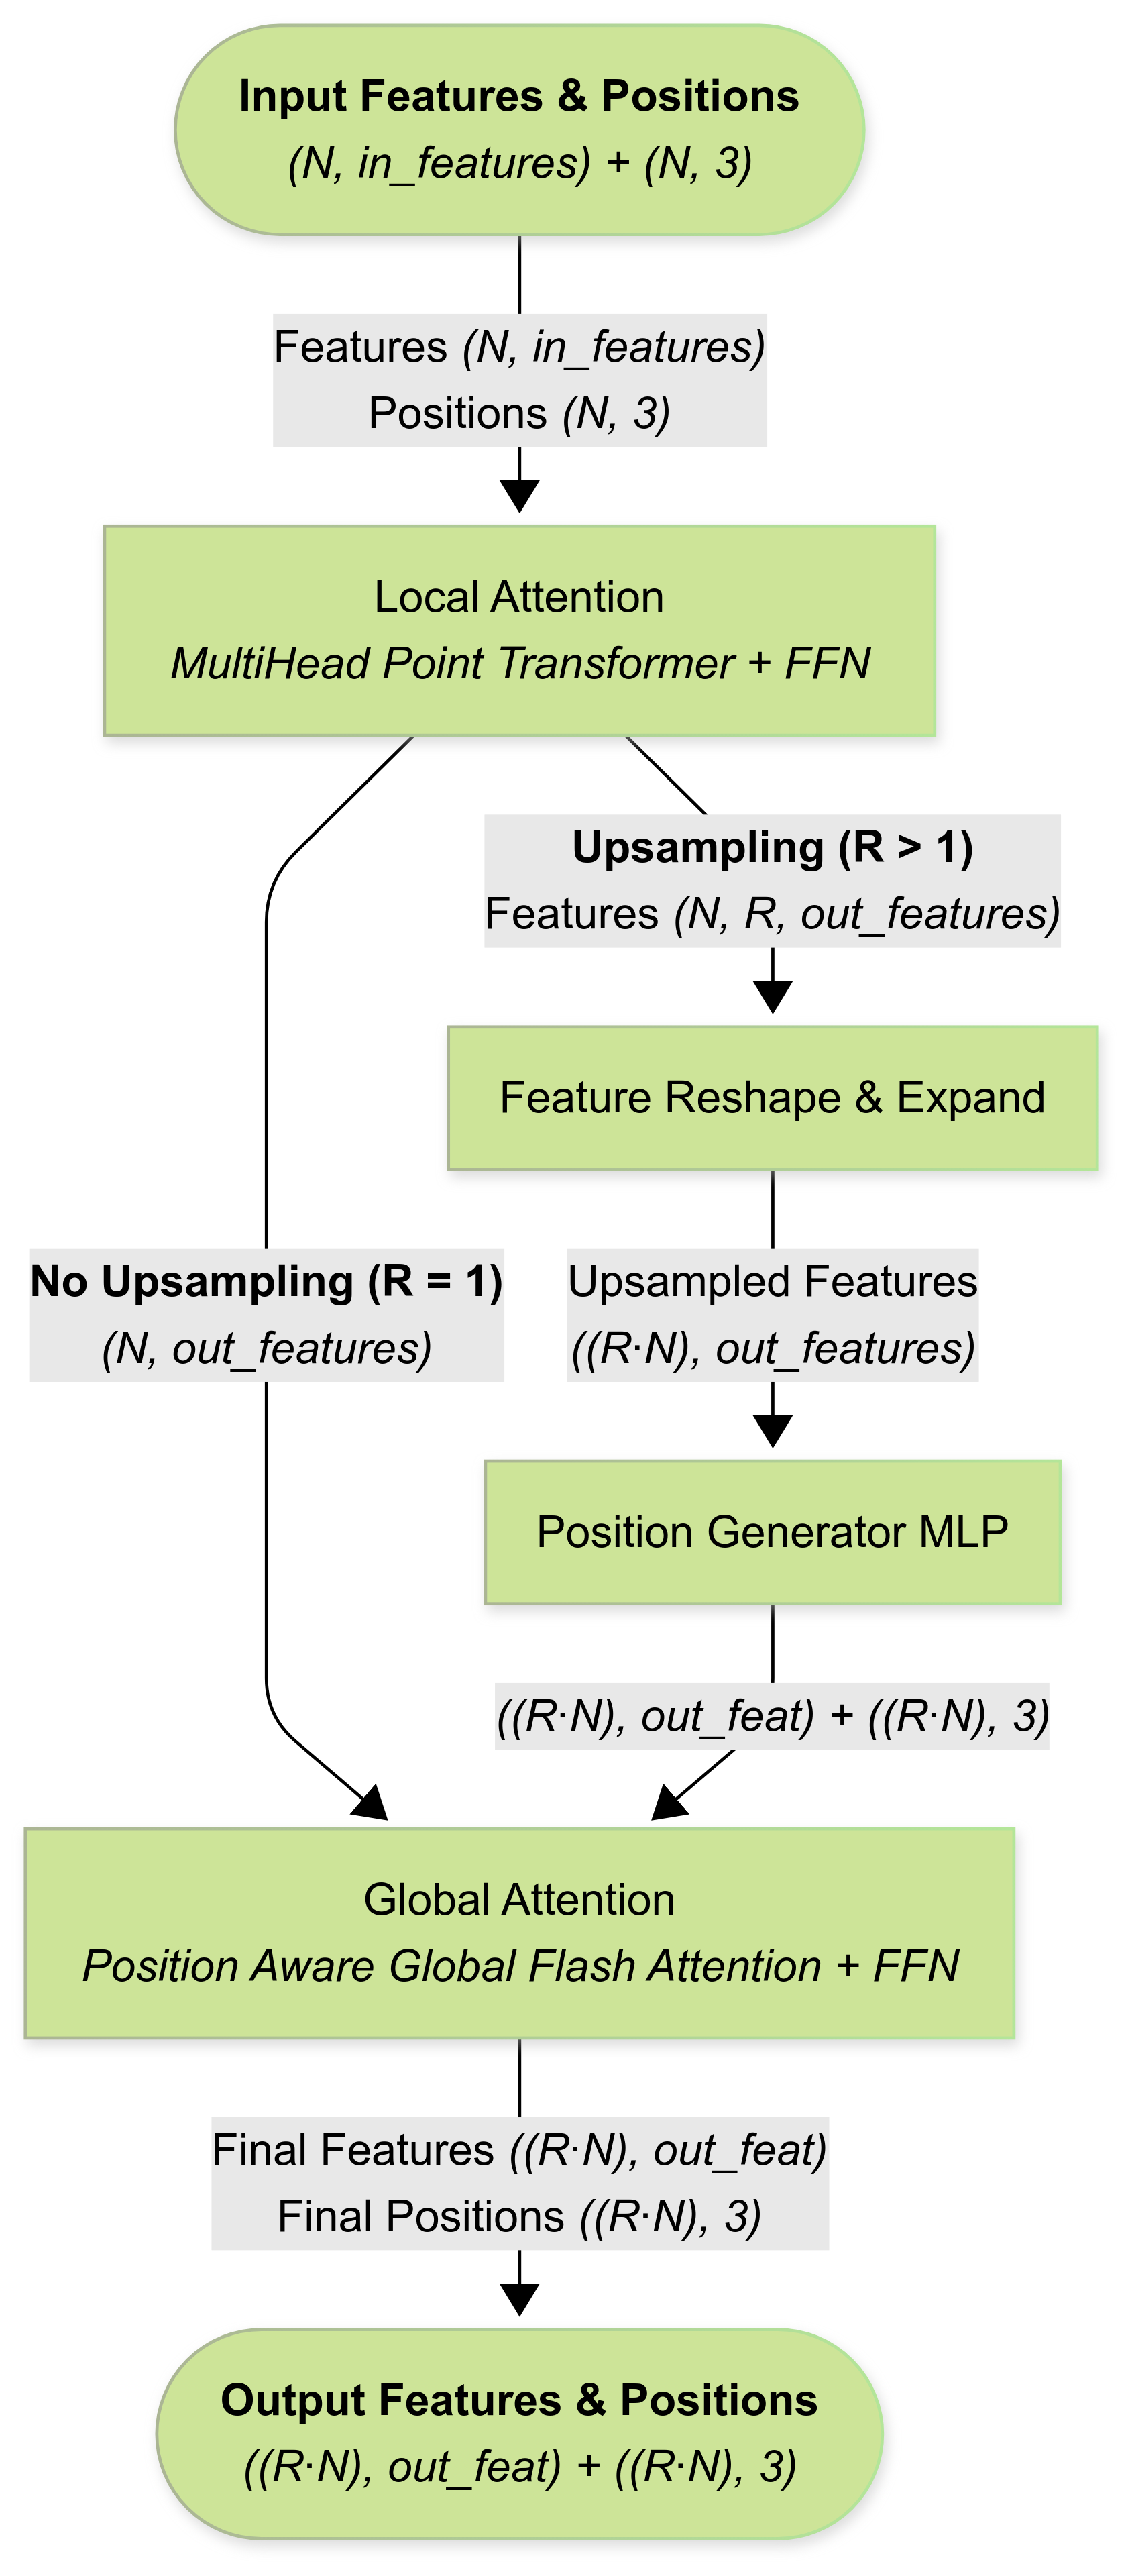
\includegraphics[trim=0mm 0mm 36mm 0mm, clip, width=0.5\textwidth]{figures/LG-PAB.png}
  \caption{\hl{Flow chart} %MDPI: To reduce the blank page. We moved the figure here. Please confirm.
 of the Local–Global Point Attention Block (LG-PAB), the core computational unit used across the feature extraction, expansion, and refinement stages. The block applies local attention via a multi-head point Transformer, optional upsampling with learned position offsets, and global multi-head FlashAttention%EE: Please check intended meaning has been retained
  for broader spatial context. A feed-forward MLP follows both the local and global attention blocks.}
  \label{fig:lgpab}
\end{figure}

\vspace{-11pt}


\begin{figure}[H]
    %\vspace{-20pt}

    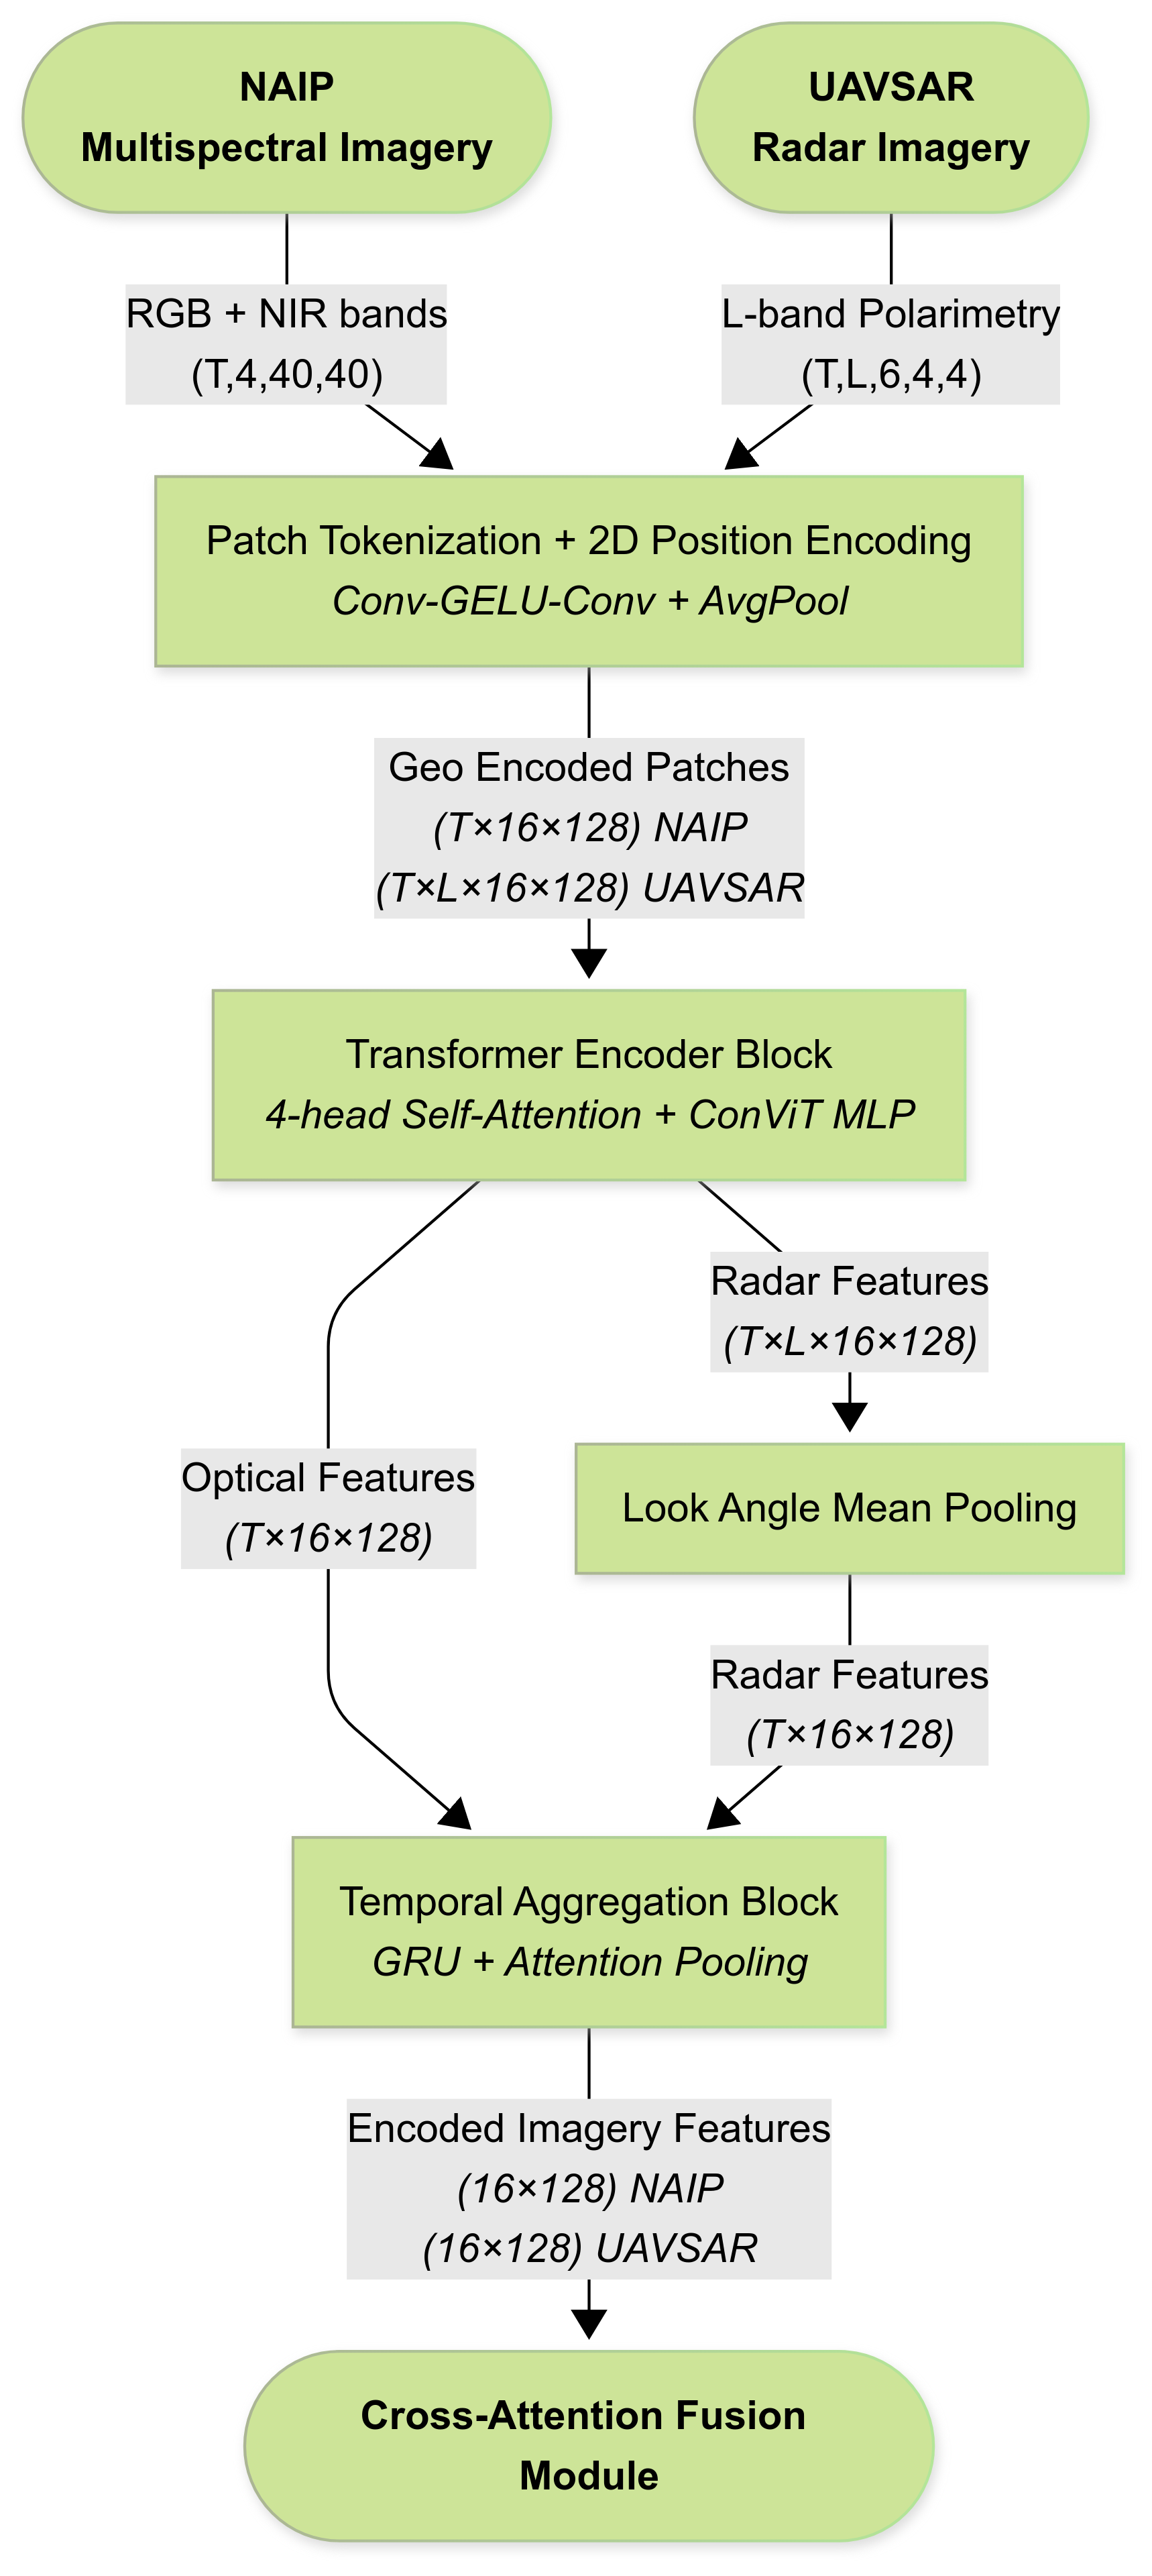
\includegraphics[trim=0mm 0mm 20mm 0mm, clip, width=0.57\linewidth]{figures/Imagery_Encoders.png}
    \caption{Architectural diagram of the imagery encoders. Image stacks from NAIP (optical) and UAVSAR (radar) pass sequentially through patch tokenization, Transformer encoder blocks for spatial context modeling, and a temporal GRU-Attention head for temporal aggregation.}
    \label{fig:imgenc}
\end{figure}





\paragraph{UAVSAR Look-Angle Mean Pooling}
\begin{itemize}[leftmargin=*]
\item \textbf{\hl{UAVSAR.}}
      Input $I_{\text{uavsar}}: (N_{\text{time}}, N_{\text{looks}}, C_{\text{uavsar}}, H_{\text{uavsar\_pr}}, W_{\text{uavsar\_pr}})$ with \mbox{$N_{\text{looks}} \leq 2$}.
      \textls[-25]{After the transformer encoder block, we average features across available look angles to produce $Z_{\text{avg}}: (N_{\text{time}}, N_{\text{patch}}, D_{\text{token}})$ before temporal processing.
      Otherwise, the pipeline \mbox{matches NAIP}.}
\end{itemize}


Both encoders output token matrices ($E_{\text{opt}}$ and $E_{\text{rad}}: (N_{\text{patch}}, D_{\text{token}})$) that are normalized and concatenated before fusion.

\newpage

\subsection{End-to-End Upsampling Pipeline}
\label{sec:pipeline}


\begin{enumerate}
\item[(1)] {\hl{Local}%MDPI: We set (1)-(6) as list. Please confirm. (MM: confirmed)
–Global Feature Extraction.}
\end{enumerate}

The sparse 3DEP cloud—concatenated with intensity, return number, and number of returns (6 attributes in total)—is processed by the first \emph{\hl{Local–Global Point Attention Block}} (Section \ref{sec:lgpab}). The output is a set of point features ($F: (N_{\text{pts}}, D_{\text{p\_feat}})$) that encode both neighborhood morphology and tile-level context.


\begin{enumerate}
\item[(2)] {Imagery Encoders.}
\end{enumerate}

Co-registered NAIP and UAVSAR chips are independently tokenized and fed to lightweight Transformer encoders ($N_{\text{patch}}$ patches, embed dim $D_{\text{token}}$). The optical encoder (RGB + NIR) outputs patch embeddings ($E_{\text{opt}}: (N_{\text{patch}}, D_{\text{token}})$), whereas the radar encoder (L-band polarimetry) outputs $E_{\text{rad}}: (N_{\text{patch}}, D_{\text{token}})$. When multiple acquisition dates exist, per-modality tokens are fused temporally via a shared GRU–attention head.

\begin{enumerate}
\item[(3)] {Cross-Attention Fusion.}
\end{enumerate}

Point features act as \emph{queries}, and image patches act as \emph{\hl{keys/values}} %EE: Please check intended meaning has been retained (MM: confirmed)
in a four-head cross-attention block.
Scaled dot-product scores are masked for patches with a centroid that is more than 8 m from the query point. The fused representation ($F_{\text{fused}}: (N_{\text{pts}}, D_{\text{p\_feat}})$) augments every point, with spectral texture and volumetric back-scatter cues improving discrimination of canopy surfaces versus gaps.

\begin{enumerate}
\item[(4)] {Feature-Guided Upsampling.}
\end{enumerate}

A second LG-PAB with a ratio of $R_{\text{up}}=2$ expands $F_{\text{fused}}$ and predicts offsets ($\Delta P$) that generate $N_{\text{pts\_up}}$ candidate coordinates%EE: Please check intended meaning has been retained (MM: confirmed)
. This stage doubles point density while maintaining local topology.

\begin{enumerate}
\item[(5)] {Feature Refinement.}
\end{enumerate}

A third LG-PAB (ratio $R_{\text{up}}=1$) re-computes local and global attention on the enlarged cloud, ironing out artifacts introduced during expansion and propagating context across newly formed neighborhoods.

\begin{enumerate}
\item[(6)] {Coordinate Decoding.}
\end{enumerate}

Finally, a four-layer MLP ($D_{\text{p\_feat}} \rightarrow 128 \rightarrow 64 \rightarrow 32 \rightarrow D_{\text{coord}}$) regresses residual offsets that are added to the upsampled positions, producing the higher resolution prediction ($\hat{P}: (N_{\text{pts\_up}}, D_{\text{coord}})$).

%-------------------------------------------------
\subsection{Training Protocol and Analysis}
\label{sec:study_design}
%-------------------------------------------------
To systematically evaluate our research questions, we established a rigorous training and analysis protocol. The full dataset, comprising tiles from both study areas, was partitioned into training, validation, and testing subsets. The training set consists of 24,000 original tiles and was expanded to 40,000 through the data augmentation process described previously. A separate set of 3792 tiles was reserved for validation during training, and a final hold-out set of 5688 tiles was used for testing and performance evaluation \mbox{(Table \ref{tab:data_prep})}.
%---------------------------------------------------------------
% 1) Dataset preparation
%---------------------------------------------------------------
\begin{table}[htbp]
  \centering
  \caption{Dataset preparation}
  \label{tab:data_prep}
  \begin{tabular}{lr}
    \toprule
    \textbf{Subset} & \textbf{Tiles} \\
    \midrule
    Training        & 24,000 original $+$ 16,000 augmented $=$ 40,000 \\
    Validation      & 3792 \\
    Test            & 5688 \\
    \bottomrule
  \end{tabular}
\end{table}

To isolate the impact of each data modality, we trained four distinct model variants (Table \ref{tab:model_variants}). A baseline model was trained using only the sparse 3DEP LiDAR input. Two single-modality models were trained by fusing the LiDAR with either NAIP optical imagery or UAVSAR radar data. Finally, a fully fused model was trained using all three data sources simultaneously.
%---------------------------------------------------------------
% 2) Model variants
%---------------------------------------------------------------
\begin{table}[htbp]
  \centering
  \begin{threeparttable}
  \caption{Model variants evaluated\footnotemark}
  \label{tab:model_variants}
  \begin{tabular}{lllr}
  \toprule
  \textbf{Variant} & \textbf{Active encoders} & \textbf{Cross-attention on} & \textbf{Parameters} \\
  \midrule
 Baseline & LiDAR only & None  & 4.7M \\
  + NAIP & LiDAR, optical  & NAIP tokens & 5.9M \\
  + UAVSAR & LiDAR, radar & UAVSAR tokens  & 5.8M \\
  Fused  & LiDAR, optical, radar & Concatenated token  & 6.8M \\
  \bottomrule
  \end{tabular}
  \footnotetext{Parameter differences relative to the baseline reflect only the additional modules enabled in each variant (e.g., imagery encoders and cross-attention fusion). The remaining architecture is unchanged to ensure a fair comparison.}
  \end{tablenotes}
  \end{threeparttable}
\end{table}


\vspace{-3pt}
All model variants were trained using an identical architecture, set of hyperparameters, and training protocol to ensure a fair comparison. Key model configuration parameters, including feature dimensions and attention head counts, are provided in Table \ref{tab:model_config_a}. The models were trained for 100 epochs on four NVIDIA L40 GPUs using the ScheduleFreeAdamW optimizer \cite{defazio_road_2024} and a density-aware Chamfer distance loss function (Equation 9 in \cite{wu_density-aware_2021}). We set the loss hyperparameter $\alpha$ to 4, adapting the recommendation in \cite{wu_density-aware_2021} for our un-normalized, meter-scale data to prevent the loss function's exponential term from saturating and causing vanishing gradients. Further details on the training protocol and hardware are listed in Table \ref{tab:training_protocol}.

\begin{table}[htbp]
  \centering
  \caption{Model-configuration parameters}
  \label{tab:model_config_a}
  %          col 1            col 2             col 3 (wraps)
  \begin{tabular}{l c p{0.55\linewidth}}
    \toprule
    \textbf{Parameter} & \textbf{Value} & \textbf{Notes} \\
    \midrule
    \multicolumn{2}{c}{\textit{Core geometry}} \\
    Point-feature dimension        & 256 & — \\
    KNN neighbours ($k$)           & 16  & Used in local attention graph \\
    Upsampling ratio ($R_{\text{up}}$) & 2 & Doubles point density per LG-PAB expansion \\
    Point-attention dropout        & 0.02 & Dropout inside global attention heads \\
    \addlinespace
    \multicolumn{2}{c}{\textit{Attention-head counts}} \\
    Extractor — local / global     & 8 / 4 & Extra local heads help expand feature set \\
    Expansion — local / global     & 8 / 4 & Extra local heads aid point upsampling \\
    Refinement — local / global    & 4 / 4 & — \\
    \addlinespace
    \multicolumn{2}{c}{\textit{Imagery encoders}} \\
    Image-token dimension          & 128 & Patch embeddings for NAIP \& UAVSAR encoders \\
    \addlinespace
    \multicolumn{2}{c}{\textit{\hl{Cross-modality fusion}}} \\
    Fusion heads                   & 4   & — \\
    Fusion dropout                 & 0.02 & — \\
    Positional-encoding dimension  & 36  & — \\
    \bottomrule
  \end{tabular}
\end{table}
\vspace{-10pt}

%---------------------------------------------------------------
% 3) Training protocol and hardware
%---------------------------------------------------------------
\begin{table}[htbp]
  \centering
  \caption{Training protocol and hardware}
  \label{tab:training_protocol}
  \begin{tabular}{lp{0.62\linewidth}}
    \toprule
    \textbf{Setting} & \textbf{Value} \\
    \midrule
    Hardware      & 4\,×\,NVIDIA L40 (48 GB) GPUs under PyTorch DDP 2.5.1 (CUDA 12.4) %MDPI: Please state which version of the software was used. Please check the whole paper and add the version number for all the software that was used for this paper. (MM: added)
 DDP \\
    Optimizer     & \textit{\hl{ScheduleFreeAdamW}} \cite{defazio_road_2024}; base LR $5\times10^{-4}$, weight-decay $10^{-4}$, $\beta_{1,2}=(0.9,0.999)$; no external LR schedule \\
    Loss function & Density-aware Chamfer distance (Equation 9 in \cite{wu_density-aware_2021}), $\alpha=4$ \\
    Batch size    & 15 tiles per GPU \\
    Epochs        & 100 \\
    Gradient clip & $\lVert g\rVert_2 \le 10$ \\
    Training time & $\approx$ 7 h per model variant \\
    Model selection & Epoch with lowest validation loss \\
    \bottomrule
  \end{tabular}
\end{table}

\vspace{-3pt}

We evaluated our research questions using non-parametric statistical tests to account for non-normality in the error distribution. For RQ1 and RQ2, we used Wilcoxon signed-rank tests to compare reconstruction error (measured by Chamfer distance) between models, with median percentage change and rank-biserial correlation as effect-size measures. For RQ3, we used Spearman rank correlations to analyze the relationship between reconstruction error and absolute change in canopy height across all models. We further split the dataset into canopy gains (N = 2423) and losses (N = 3264) to examine potential asymmetries in error patterns. Fisher r-to-z transformations were used to statistically compare correlation coefficients between models. All significance values are reported at $\alpha$=0.05, with bold values indicating statistically significant results.
For each tile, net canopy height change was calculated as the difference in the mean 95th percentile point height (z-value) across 2 m × 2 m grid cells between the UAV LiDAR and 3DEP clouds (N=5687; one tile removed due to a spurious below-ground return in 3DEP preventing canopy-change computation).
%%%%%%%%%%%%%%%%%%%%%%%%%%%%%%%%%%%%%%%%%%
\section{Results}

A summary of the reconstruction performance, measured by Chamfer distance (CD), across all models is presented in Table \ref{tab:descriptive_stats}.The 3DEP LiDAR-only baseline model yields a markedly lower CD and a tighter distribution than the raw, sparse input (Figure \ref{fig:baseline_v_input_boxplot}; Figure \ref{fig:baseline_pt_cloud_example}); however, because CD can vary with sampling density and point counts, we present this contrast as a qualitative soundness check rather than a normalized comparison. When comparing the performance across all models (Figure \ref{fig:boxplot_model_comparison}), the fused model consistently achieved the lowest median error and smallest interquartile range, indicating the most robust performance. To address our first research question (RQ1) on the impact of individual modalities, we compared the error distributions of the single-modality models against the baseline \mbox{(Table \ref{tab:rq1_rq2_combined})}.


\begin{table}[H]
\centering
\caption{Descriptive statistics for Chamfer distance across all model variants (see Table \ref{tab:model_variants}).}
\begin{tabularx}{\textwidth}{lCCCC}
\toprule
\textbf{Model} & \textbf{Mean CD (m)} & \textbf{Median CD (m)} & \textbf{Std Dev (m)} & \textbf{IQR (m)} \\
\midrule
Input & 2.568 & 0.858 & 6.852 & 1.540 \\
Baseline & 1.043 & 0.340 & 5.717 & 0.465 \\
NAIP & 0.993 & 0.316 & 5.542 & 0.421 \\
UAVSAR & 0.924 & 0.331 & 5.505 & 0.437 \\
Fused & 0.965 & 0.298 & 5.753 & 0.393 \\
\bottomrule
\end{tabularx}
\label{tab:descriptive_stats}
\end{table}

\vspace{-10pt}



\begin{table}[H]
\centering
\caption{RQ1 and RQ2: Impact of single and fused modalities on reconstruction error.}
\label{tab:rq1_rq2_combined}
\begin{tabularx}{\textwidth}{lCC}
\toprule
\textbf{Comparison} & \textbf{Median Change (\%)} & \textbf{Effect Size} \\
\midrule
\multicolumn{3}{l}{\textit{\hl{RQ1: Single Modality vs. Baseline}}} \\
\quad NAIP vs. Baseline & \textbf{0.5} (\emph{p} $<$ 0.001) & \textbf{0.088} \\
\quad UAVSAR vs. Baseline & \textbf{0.3} (\emph{p} $<$ 0.001) & \textbf{0.062} \\
\midrule
\multicolumn{3}{l}{\textit{\hl{RQ2: Fused Modality vs. Best Single Modality}}} \\
\quad Fused vs. NAIP & \textbf{0.7} (\emph{p} $<$ 0.001) & \textbf{0.133} \\
\bottomrule
\end{tabularx}

\vspace{2pt}
\footnotesize\textbf{Note:} Bold values indicate statistical significance at \emph{p} $\leq 0.05$
\end{table}

\vspace{-14pt}

\begin{figure}[H]

    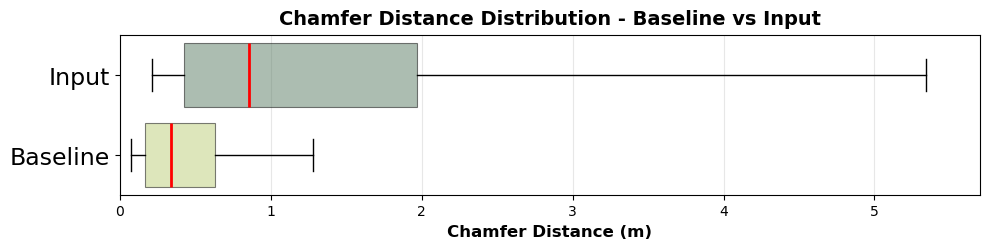
\includegraphics[width=0.99\linewidth]{figures/baseline_v_input_boxplot.png}
    \caption{Distribution of Chamfer distance (CD) reconstruction errors comparing raw input data to the 3DEP LiDAR-only baseline model, each evaluated against the reference. Horizontal boxplots show the median (red line), interquartile range (colored boxes), and 10th–90th percentile whiskers; outliers beyond the 90th percentile are excluded. The baseline model shows a lower median CD (0.340 m vs. 0.858 m) with a tighter distribution. (Note: CD can vary with sampling density and point counts; since the input and predictions (2$\times$ upsampled) differ in size relative to the reference, these magnitudes are not a normalized comparison and are shown for qualitative context.)}
    \label{fig:baseline_v_input_boxplot}
\end{figure}

\begin{figure}[H]

\begin{adjustwidth}{-\extralength}{0cm}
\centering %% If there is a figure in wide page, please release command \centering, for Table, ``\textwidth" should be ``\fulllength"
\includegraphics[width=0.98\linewidth]{figures/baseline_prediction_example.png}
\end{adjustwidth}
    \caption{\hl{A} %MDPI: 1. Commas are only used for numbers with five or more digits. We removed them in four-digit numbers in the figure. Please confirm. 2. Please confirm if explanation should be added for colors in the image. (MM: Finen as-is)
 comparison of baseline (3DEP LiDAR only) model output vs. input.}
    \label{fig:baseline_pt_cloud_example}
\end{figure}


\vspace{-10pt}

\begin{figure}[H]
    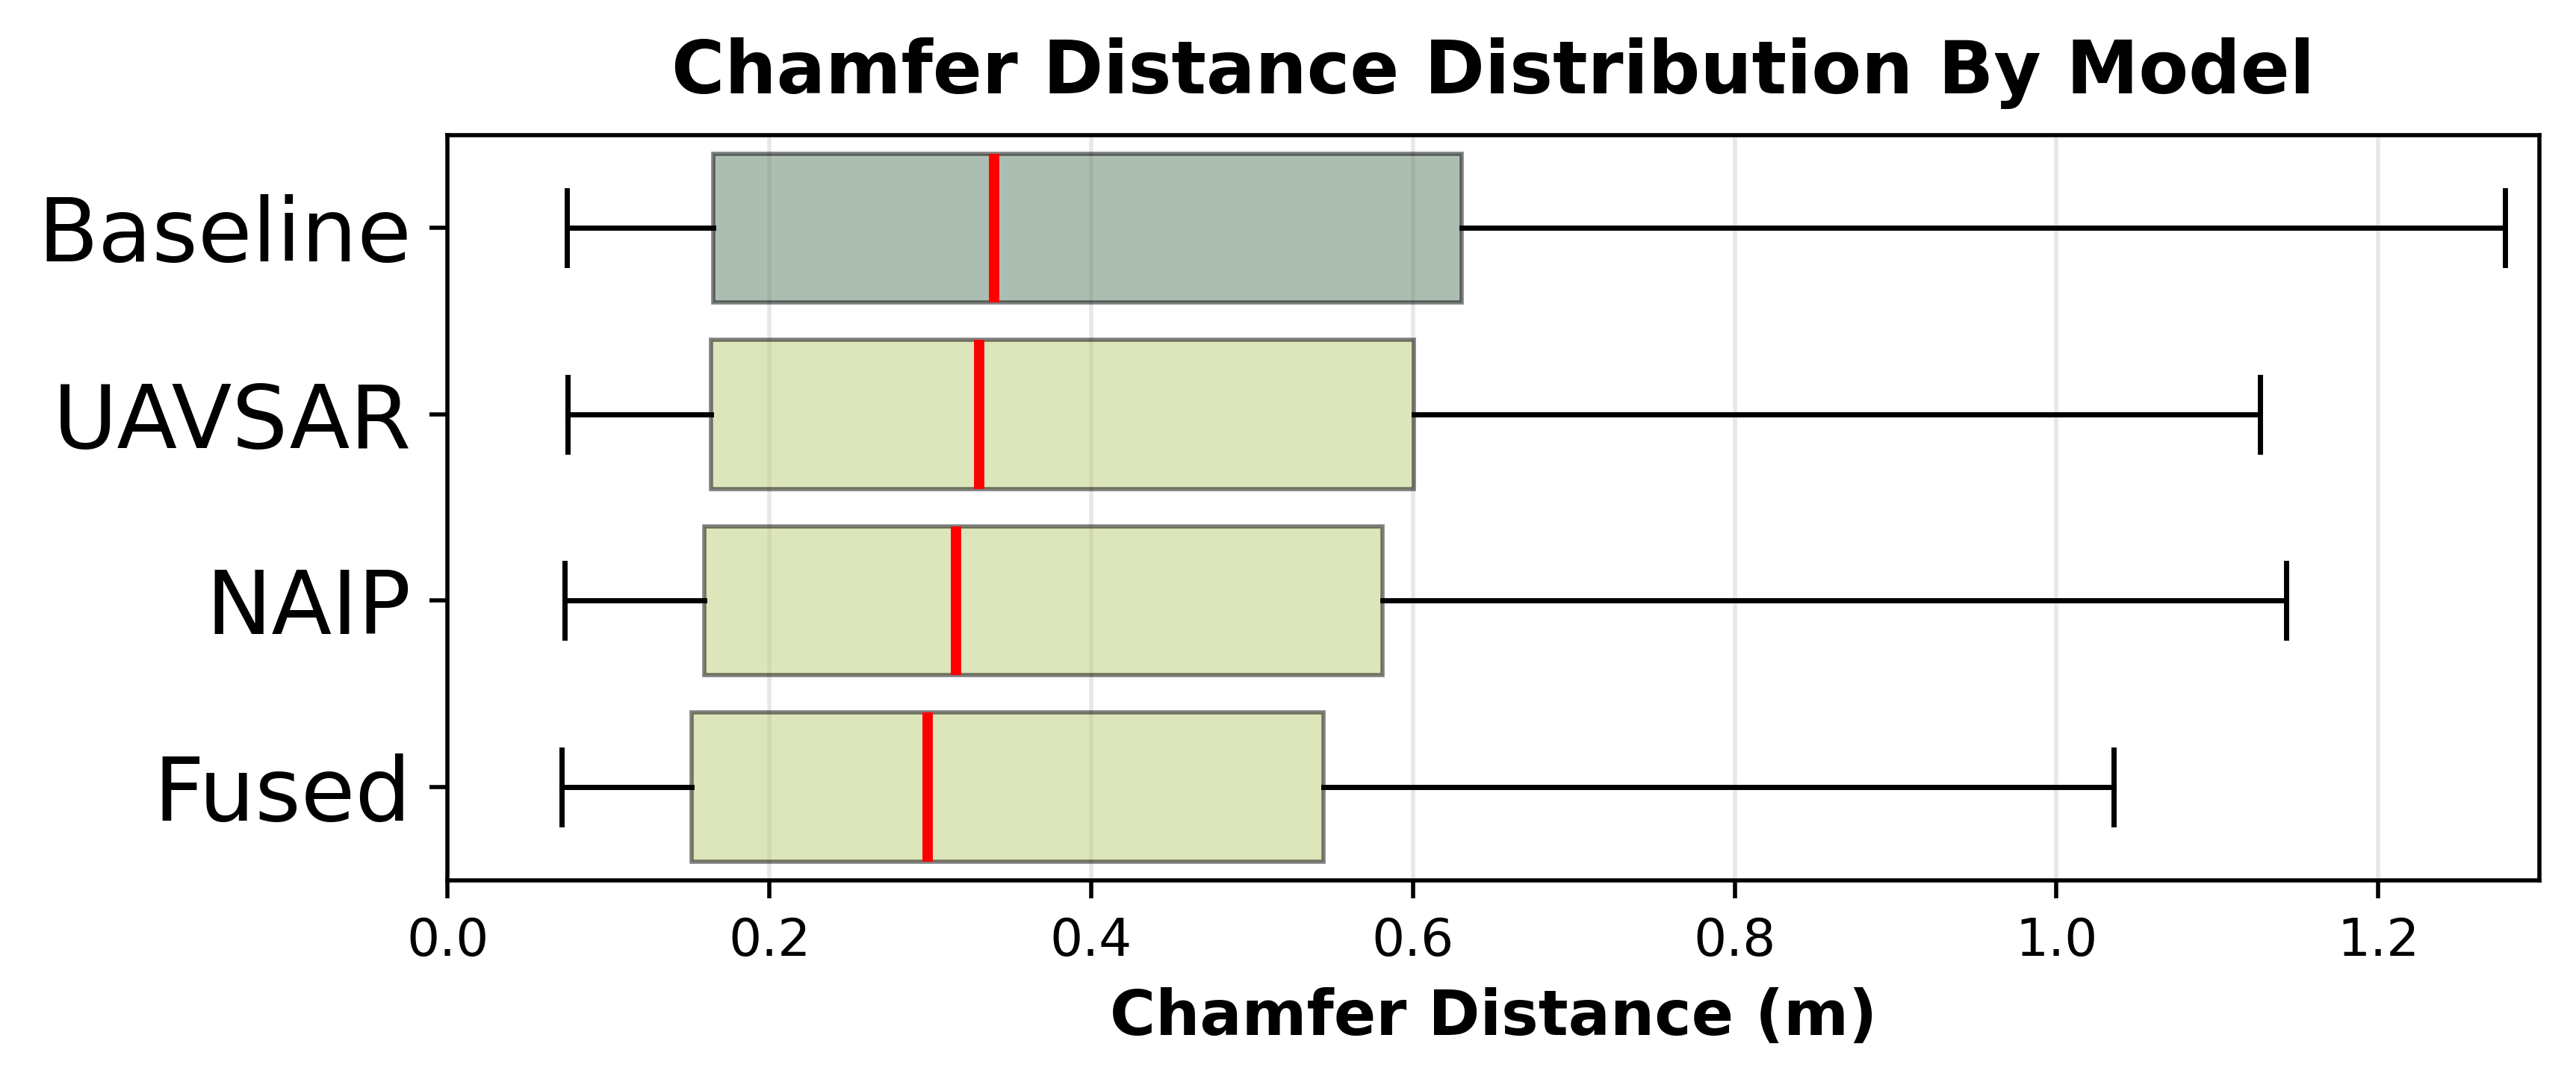
\includegraphics[width=0.75\linewidth]{figures/boxplot_by_model.png}
    \caption{Distribution of Chamfer distance reconstruction errors across point-cloud upsampling models. Horizontal box plots show median (red line), interquartile range (colored boxes), and \mbox{10th--90th percentile} whiskers for models trained with different input modalities. All models demonstrate substantial improvement over the LiDAR-only baseline, with the fused model achieving the lowest median error (0.298 m) and tightest distribution. Outliers beyond the 90th percentile are excluded \mbox{for clarity}.}
    \label{fig:boxplot_model_comparison}
\end{figure}



Both high-resolution optical imagery (NAIP) and L-band SAR imagery significantly reduced reconstruction error compared to the LiDAR-only baseline, with optical imagery providing slightly larger improvements (0.5\% vs. 0.3\%). While statistically significant, the modest effect sizes (0.088 and 0.062 respectively) suggest that single-modality improvements over the baseline upsampling approach are limited in magnitude or may be concentrated in a limited number of tiles. Next, to evaluate our second research question (RQ2), we assessed whether fusing both imagery types yielded additional benefits over the best single-modality model (Table \ref{tab:rq1_rq2_combined}).


The fusion of both optical and SAR imagery yielded additional reconstruction accuracy gains (0.7\% median reduction) beyond using NAIP alone, with a stronger effect size (0.133) than either individual modality achieved in RQ1. This statistically significant improvement supports our hypothesis that the two modalities contain complementary information that can be effectively combined through attention-based fusion. The results demonstrate that multi-modality approaches can leverage different sensing capabilities to achieve superior point-cloud reconstruction (Figure \ref{fig:model_output_example}).


\vspace{-3pt}


\begin{figure}[H]
\begin{adjustwidth}{-\extralength}{0cm}
\centering
    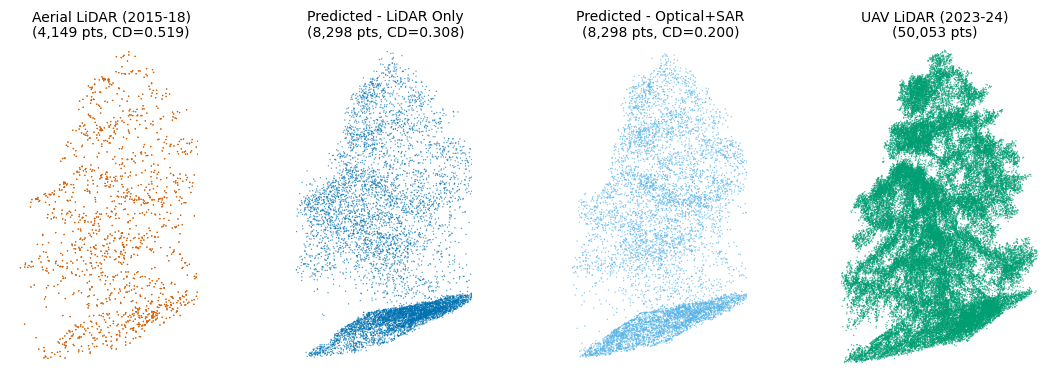
\includegraphics[width=1\linewidth]{figures/model_output_example.png}
    \end{adjustwidth}
    \caption{\hl{Example} %MDPI: 1. Please change the hyphen (-) between numbers into an en dash (−, “U+2013”), e.g., “2015-18” should be “2015–18”. 2. Commas are only used for numbers with five or more digits. Please remove them from the four-digit numbers in the figure, e.g., “1,200” should be “1200”. 3. Please confirm if explanation should be added for colors in the image. (MM: 1. Changed as requested. 2. Unable to remove. 3. Fine as-is)
 tile where no major vegetation change occurred between the 3DEP aerial LiDAR (2015−2018) and UAV LiDAR (2023−2024). The optical + SAR fusion model more accurately recovers fine-scale canopy structure compared to the LiDAR-only model, producing a point cloud that more closely matches the UAV LiDAR reference (lower Chamfer distance).}
    \label{fig:model_output_example}
\end{figure}




Finally, to evaluate our third research question (RQ3) on the impact of vegetation change, we correlated model error with the magnitude of canopy height changes between the legacy 3DEP and recent UAV LiDAR surveys. Table \ref{tab:rq3_results} shows the overall Spearman rank correlations. To investigate this relationship further, we split the dataset into areas of net canopy gain and net canopy loss, with the results of this extended analysis presented in Table \ref{tab:rq3_extended_results}.

\begin{table}[H]

\caption{RQ3: Correlation between reconstruction error and canopy height change.}
\begin{tabularx}{lCC} %MM: Please do not make table textwidth. Adds too much whitespace and hinders readability.
\toprule
\textbf{Model} & \textbf{Spearman \boldmath{$\rho$}} & \textbf{\textit{p}-Value} \\
\midrule
Baseline & \textbf{\hl{0.650} %MDPI: Please add an explanation for the use of bold in the table footer. If the bold is unnecessary, please remove it. Please check all bold in the table. (MM: added footer)
} & \emph{p} $<$ 0.001 \\
NAIP & \textbf{0.612} & \emph{p} $<$ 0.001 \\
UAVSAR & \textbf{0.628} & \emph{p} $<$ 0.001 \\
Fused & \textbf{0.582} & \emph{p} $<$ 0.001 \\
\midrule
Baseline vs. NAIP (z) & \textbf{3.377} & \emph{p} $<$ 0.001 \\
Baseline vs. UAVSAR (z) & \textbf{1.999} & \emph{p} = 0.046 \\
Baseline vs. Fused (z) & \textbf{5.868} & \emph{p} $<$ 0.001 \\
\bottomrule
\end{tabularx}
\label{tab:rq3_results}
\footnotesize\textbf{Note:} Bold values indicate statistical significance at \emph{p} $\leq 0.05$.
\end{table}
\vspace{-10pt}

\begin{table}[H]

\caption{\hl{RQ3} %MDPI: We revised the line format in the table. Please confirm this revision. (MM: Please do not make table textwidth. Adds too much whitespace and hinders readability.)
 extended: Correlation between reconstruction error and canopy height changes (gains vs. losses).}
\begin{tabularx}{lCCCC}
\toprule
\multirow{2.35}{*}{\textbf{Model}} & \multicolumn{2}{c}{\textbf{Canopy Gains (N = 2423)}} & \multicolumn{2}{c}{\textbf{Canopy Losses (N = 3264)}} \\
\cmidrule{2-5}
 & \textbf{Spearman \boldmath{$\rho$}} & \textbf{\emph{p}-Value} & \textbf{Spearman \boldmath{$\rho$}} & \textbf{\emph{p}-Value} \\
\midrule
Baseline & \textbf{\hl{0.601} %MDPI: Please add an explanation for the use of bold in the table footer. If the bold is unnecessary, please remove it. Please check all bold in the whole table.
} & \emph{p} $<$ 0.001 & \textbf{0.671} & \emph{p} $<$ 0.001 \\
NAIP & \textbf{0.586} & \emph{p} $<$ 0.001 & \textbf{0.621} & \emph{p} $<$ 0.001 \\
UAVSAR & \textbf{0.597} & \emph{p} $<$ 0.001 & \textbf{0.637} & \emph{p} $<$ 0.001 \\
Fused & \textbf{0.587} & \emph{p} $<$ 0.001 & \textbf{0.580} & \emph{p} $<$ 0.001 \\
\midrule
Baseline vs. NAIP (z) & 0.825 & \emph{p} = 0.409 & \textbf{3.440} & \emph{p} $<$ 0.001 \\
Baseline vs. UAVSAR (z) & 0.233 & \emph{p} = 0.816 & \textbf{2.406} & \emph{p} = 0.016 \\
Baseline vs. Fused (z) & 0.768 & \emph{p} = 0.442 & \textbf{6.074} & \emph{p} $<$ 0.001 \\
\bottomrule
\end{tabularx}
\label{tab:rq3_extended_results}
\footnotesize\textbf{Note:} Bold values indicate statistical significance at \emph{p} $\leq 0.05$.
\end{table}
\vspace{-3pt}

All models showed strong correlations with absolute canopy height change, confirming that reconstruction error systematically increases with vegetation structure changes since to the original LiDAR collection%EE: Please check intended meaning has been retained (MM: reverted some changes, but kept most)
. The baseline model exhibited the strongest correlation with canopy change ($\rho=0.650$), while the fused model showed the weakest correlation ($\rho=0.582$), with this difference being statistically significant ($z=5.868$, $p<0.001$). Importantly, the extended analysis revealed that this pattern was driven primarily by canopy losses, where the baseline model performed significantly worse than all other models, particularly the fusion approach ($z=6.074$, $p<0.001$), while for canopy gains, all models performed similarly, without statistically significant differences. These findings partially support our hypothesis that advanced models better mitigate error from canopy changes---specifically for canopy removal scenarios, where legacy LiDAR contains no information about the removed vegetation (Figures \ref{fig:single_veg_loss_example} and \ref{fig:error_vs_cnpy_chng}). For canopy gains the limited separation is consistent with our original reasoning: most growth cases represent incremental vertical or volumetric accretion within an existing structural envelope already partly encoded in the sparse legacy LiDAR, allowing even the baseline to extrapolate plausibly. Ancillary optical and SAR cues add comparatively little discriminative signal for these modest positive changes, whereas abrupt canopy removal creates a true information void that fused imagery helps fill.


\vspace{-3pt}

\begin{figure}[H]
\begin{adjustwidth}{-\extralength}{0cm}
    \centering
    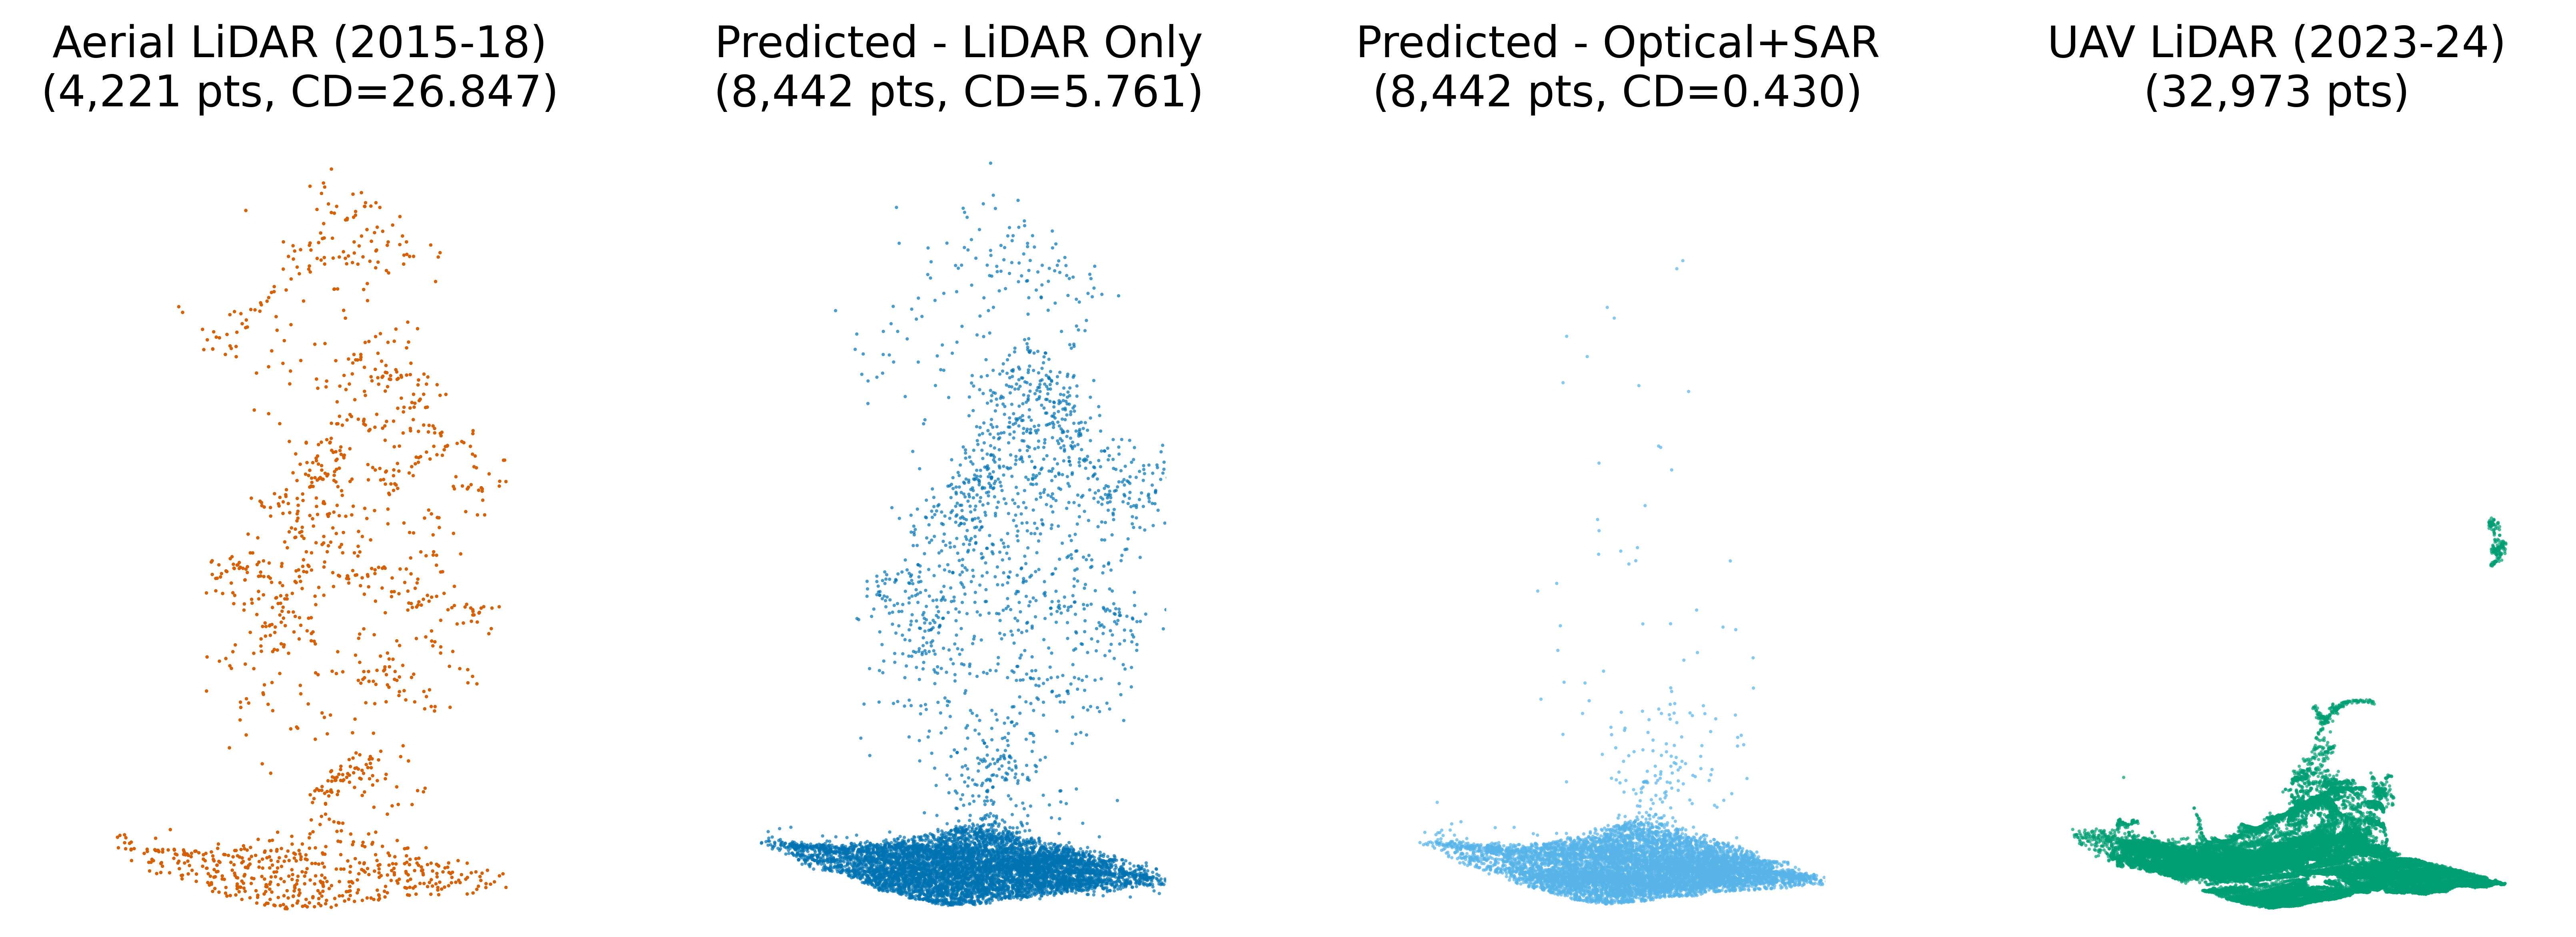
\includegraphics[width=0.85\linewidth]{figures/single_veg_loss_example.png}
    \end{adjustwidth}
    \caption{\hl{Example} %MDPI: 1. Please change the hyphen (-) between numbers into an en dash (−, “U+2013”), e.g., “2015-18” should be “2015–18”. 2. Commas are only used for numbers with five or more digits. Please remove them from the four-digit numbers in the figure, e.g., “1,200” should be “1200”. 3. Please confirm if explanation should be added for colors in the image. (MM: 1. Changed as requested. 2. Unable to remove. 3. Fine as-is)
 tile illustrating vegetation structure change between legacy aerial LiDAR (\mbox{2015−2018}) and recent UAV LiDAR (2023−2024). The optical + SAR fusion model accurately reconstructs the canopy loss visible in the UAV LiDAR reference, whereas the LiDAR-only model retains outdated structure from the earlier survey. This highlights the value of multi-modal imagery in correcting legacy LiDAR and detecting structural change.}
    \label{fig:single_veg_loss_example}
\end{figure}


\vspace{-11pt}

\begin{figure}[H]
\begin{adjustwidth}{-\extralength}{0cm}
    \centering
    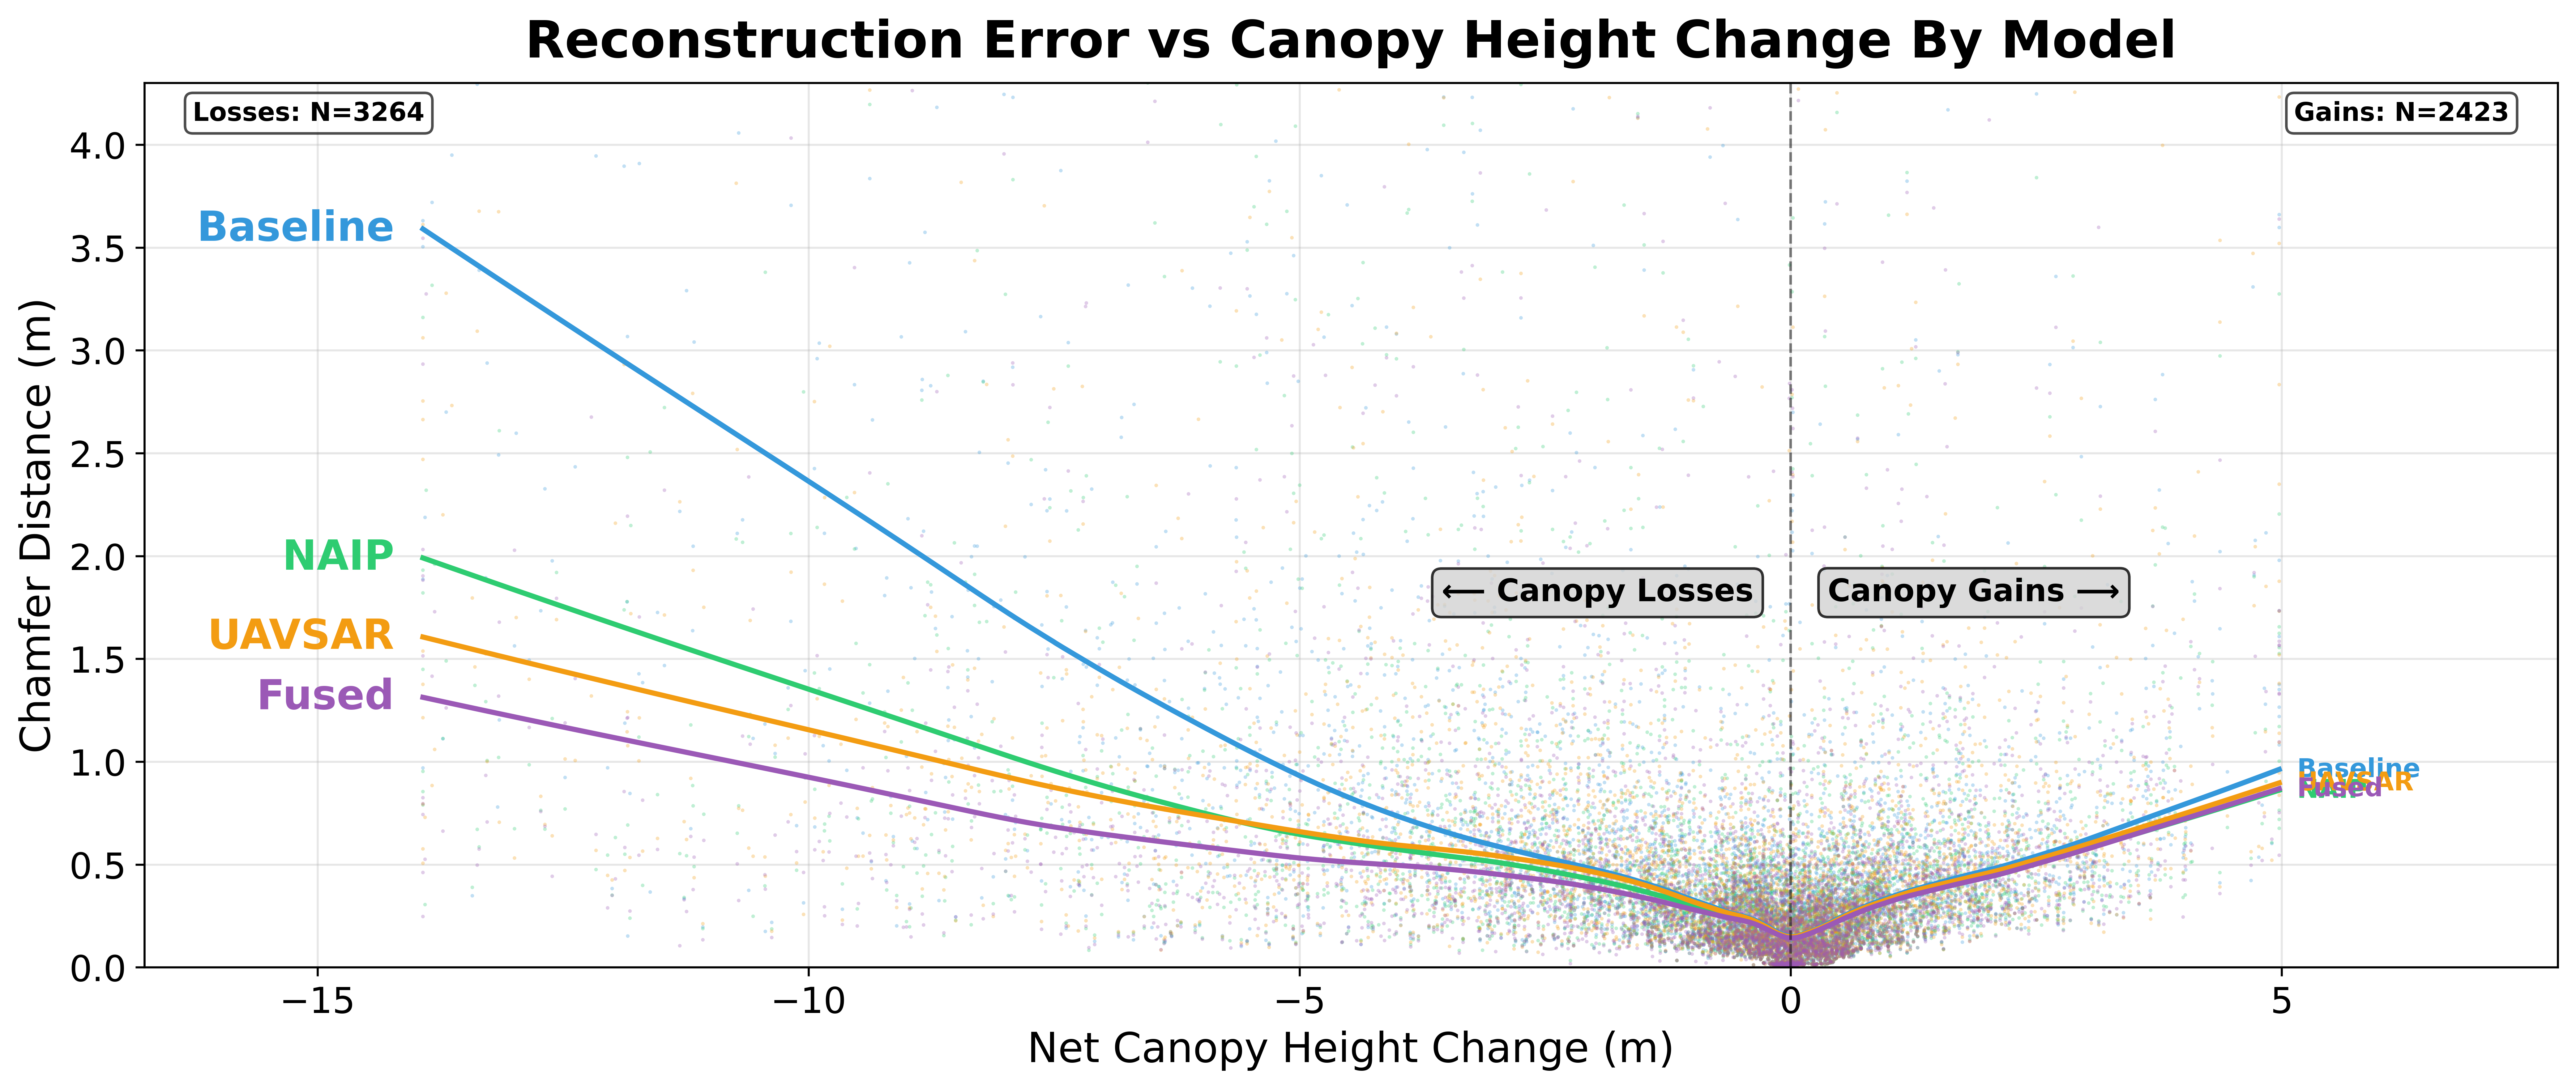
\includegraphics[width=1\linewidth]{figures/error_vs_cnpy_chng.png}
    \end{adjustwidth}
    \caption{\hl{Relationship} %MDPI: Please confirm whether the overlapping content in this figure affects scientific understanding and if it does, please revise it.(MM: Overlap is trivial and does not affect understanding. Also figure should be full width to be legible)
 between point-cloud reconstruction error (Chamfer distance) and net canopy height change since the original LiDAR survey. Scatter points show individual sample tiles \mbox{(N = 5687)} with LOWESS trend lines for each model; outliers above the 99.5th percentile for both error and height change metrics were excluded for visual clarity. Negative values represent canopy losses, while positive values represent gains. The baseline model (blue) shows substantially higher error rates for large canopy losses compared to models incorporating additional remote sensing data (NAIP optical, UAVSAR radar, and fused approaches), while all models perform similarly for \mbox{canopy gains}.}
    \label{fig:error_vs_cnpy_chng}
\end{figure}

%%%%%%%%%%%%%%%%%%%%%%%%%%%%%%%%%%%%%%%%%%
\section{Discussion}



This study demonstrates the significant potential of attention-based deep learning models to enhance sparse and outdated airborne LiDAR point clouds by fusing them with more frequently acquired optical (NAIP) and synthetic aperture radar (UAVSAR) imagery. Our findings directly address the critical need for up-to-date, high-resolution 3D vegetation structure information in applications like wildfire risk modeling and ecological monitoring.

The core success of our approach lies in the effective fusion of multi-modal data. As hypothesized (RQ1), both NAIP optical imagery and L-band UAVSAR imagery, when individually integrated, improved point-cloud reconstruction accuracy compared to a baseline model relying solely on sparse LiDAR. NAIP, with its finer spatial resolution, offered a slightly greater enhancement, likely due to its ability to delineate canopy edges and small gaps with high fidelity. However, the true advancement was observed when these modalities were combined (RQ2). The fused model, leveraging both NAIP's textural detail and UAVSAR's structural sensitivity, outperformed single-modality enhancements. This confirms our hypothesis that these sensors provide complementary rather than redundant information and that the cross-attention mechanisms within our architecture can effectively identify and leverage these synergistic relationships. This synergy is particularly valuable for capturing the complex, heterogeneous nature of vegetation.

Our investigation into temporal dynamics (RQ3) revealed that all models, including the baseline, exhibited increased reconstruction error in areas with substantial canopy change since the initial LiDAR survey. This is expected, as the input LiDAR reflects a past state. However, the fused model demonstrated the most robust performance, showing a significantly weaker correlation between error and the magnitude of canopy change, especially in areas of canopy loss. This is a crucial finding: by incorporating more recent imagery, particularly optical data that clearly depicts vegetation absence, the model can more effectively correct for outdated LiDAR information. The baseline model, lacking this current-state information, struggled most in loss scenarios. Even in areas of canopy growth, while not as pronounced as with loss, the image-informed models offered an advantage by providing cues about new or denser vegetation that the original sparse LiDAR could not capture. This capacity to ``update'' historical LiDAR datasets significantly enhances their utility for long-term monitoring and management, especially in landscapes prone to rapid changes from disturbances or growth.

The developed Local--Global Point Attention Block (LG-PAB) proved to be a robust architectural component. Its ability to capture both fine-grained local details through neighborhood-level self-attention and broader structural coherence via global attention across the entire point patch is central to its success. This hierarchical attention is well-suited to the fractal-like patterns often observed in natural vegetation.

Despite these promising results, some limitations exist. The improvements, while statistically significant, were modest in terms of percentage change in Chamfer distance. This suggests that while fusion helps, there might be inherent limits to the upsampling of very sparse LiDAR or that the current metrics may not fully capture all aspects of structural improvement relevant to ecological applications.

We acknowledge that perfect cross-sensor alignment is not guaranteed in practice. We deliberately selected established, well-orthorectified public datasets (3DEP, NAIP, UAVSAR) to minimize gross misregistration, and we chose point-to-image cross-attention (with a modest spatial proximity mask) rather than direct concatenation of co-located patch features partly because attention is more tolerant to small horizontal offsets and timing differences among inputs: it allows each point to attend to the most informative nearby patch rather than a single fixed location. We did not conduct a formal misregistration sensitivity study, which we identify as future work.

More broadly, our experiments and training were conducted in Southern California's Mediterranean ecosystems; model performance—and the relative contributions of optical versus radar—may differ in other biomes with distinct vegetation structure and phenology. Accordingly, out-of-domain application without additional high-density LiDAR may degrade performance; however, incorporating UAV LiDAR from new biomes into training is a straightforward path to broader generalization.

Beyond the primary 2× upsampling task, we also conducted a preliminary investigation into the model's potential for higher ratio densification (8×
). This exploratory model was scaled up significantly, with larger feature dimensions (512 points and 192 images%EE: Please check intended meaning has been retained
), more local attention heads for extraction and expansion (16)%MDPI: Please check if it is a reference citation. If so, please revise it into the right format. (Not a reference citation. Refers to number of attention heads)
 , and additional LG-PAB layers (six total)
, and a total of ~125 M parameters. With our hardware, this increased model size necessitated reducing the batch size to one per GPU. The results (Figure \ref{fig:upsampling_comparison_8x}) show that the architecture can, indeed, produce highly dense outputs that qualitatively approach the reference data. Appendix \ref{app1} provides further qualitative examples from both the standard 2×
 and experimental 8× models, illustrating their performance across different vegetation change scenarios (Figures \ref{fig:appendix_growth1}--\ref{fig:appendix_loss}).

 \vspace{-6pt}

\begin{figure}[H]
    \begin{adjustwidth}{-\extralength}{0cm}
    \centering
    \includegraphics[width=1\linewidth]{figures/example_8x_v_2x.png}
    \end{adjustwidth}
    \caption{\hl{Comparison} %MDPI: 1. Commas are only used for numbers with five or more digits. We removed them in four-digit numbers in the figure. Please confirm. 2. Please confirm if explanation should be added for colors in the image. (MM: 1. Thank you, 2. Fine as-is)
 of the standard 2× upsampling model (optical + SAR, 6.8 million parameters) output versus a preliminary high-density 8× model (optical + SAR, 125 million parameters).}
    \label{fig:upsampling_comparison_8x}
\end{figure}

\newpage

A recommended area for future research involves adapting the validated multi-modal feature extraction pipeline for direct prediction of key vegetation structure rasters, such as Canopy Height Models (CHMs), canopy cover, Above-Ground Biomass (AGB), and fuel types. Such an adaptation would entail replacing the current point-cloud generation head with task-specific regression or classification heads, potentially broadening the practical applicability of this work. Integrating geometric priors like Digital Surface Models (DSMs) and Digital Terrain Models (DTMs) into the loss function also represents a valuable direction. This could not only enforce greater structural realism but also enable the calculation of reconstruction error at various canopy strata, offering deeper insights into model performance. Furthermore, fine-tuning emerging foundation-model vision Transformers, such as the Clay model \cite{clay_model_v1p5}, as shared encoders for NAIP and UAVSAR imagery warrants exploration to leverage large-scale pretraining for enhanced feature representation. Complementary investigations could include a thorough evaluation of the UAVSAR encoder, particularly with respect to the optimization of multi-look fusion beyond simple averaging and assessment of resampling impacts, alongside ablation studies on the LG-PAB and imagery encoders to pinpoint key architectural contributions and guide further optimization. Future architectural research could also explore simplifying the Local--Global Point Attention Block into a Pure Point Attention Block by replacing the k-NN local attention with a global attention module. For greater scalability, this could be paired with a latent attention \mbox{strategy \cite{liu2024deepseek}} to bypass the quadratic complexity inherent to self-attention.


%%%%%%%%%%%%%%%%%%%%%%%%%%%%%%%%%%%%%%%%%%
\section{Conclusions}

This research successfully demonstrates that attention-based deep learning, leveraging our novel Local--Global Point Attention Block, can significantly enhance sparse airborne LiDAR point clouds in vegetated landscapes through the fusion of more recent optical and radar imagery. We have shown that while individual imagery modalities provide benefits, their combined use yields superior reconstruction accuracy, particularly in mitigating errors arising from vegetation changes over time. Specifically, high-resolution optical imagery (NAIP) proved slightly more effective as a standalone ancillary dataset than L-band SAR within our framework, but the fusion of both offered the best performance, validating the complementary nature of these sensors. A key contribution is the model's ability to substantially reduce reconstruction degradation in areas of vegetation loss, thereby increasing the utility of historical LiDAR archives. This study presents a novel approach to direct 3D point-cloud upsampling using multi-modal fusion in complex natural environments, moving beyond prevalent raster-based enhancement techniques and paving the way for more accurate and timely assessments of vegetation structure.
%%%%%%%%%%%%%%%%%%%%%%%%%%%%%%%%%%%%%%%%%%


%%%%%%%%%%%%%%%%%%%%%%%%%%%%%%%%%%%%%%%%%%
\vspace{6pt}

%%%%%%%%%%%%%%%%%%%%%%%%%%%%%%%%%%%%%%%%%%

\authorcontributions{Conceptualization, M.M. and D.S.; methodology, M.M.; software, M.M.; validation, M.M.; formal analysis, M.M.; investigation, M.M. and D.S.; resources, D.S. and J.F.; data curation, M.M.; writing---original draft preparation, M.M.; writing---review and editing, D.S. and J.F.; visualization, M.M.; supervision, D.S. and J.F.; project administration, D.S. and J.F.; funding acquisition, D.S. and J.F. All authors have read and agreed to the published version of the manuscript.}

\funding{\hl{Funding} %MDPI: Information regarding the funder and the funding number should be provided. Please check the accuracy of funding data and any other information carefully.(MM: confirmed)
 for the research was provided by California Climate Action Matching Grants, University of California, Office of the President (grant \#R02CM708 to M. Jennings, SDSU (PI) and JF)%EE: Please check intended meaning has been retained (MM: confirmed)
 . DS gratefully acknowledges funding from the NASA FireSense program (Grant \# 80NSSC24K0145), the NASA FireSense Implementation Team (Grants \#80NSSC24K1320),the NASA Land-Cover/Land Use Change program (Grant \#NNH21ZDA001N-LCLUC), the EMIT Science and Applications Team program (Grant \#80NSSC24K0861), the NASA Remote Sensing of Water Quality program (Grant \#80NSSC22K0907), the NASA Applications-Oriented Augmentations for Research and Analysis Program (Grant \#80NSSC23K1460), the NASA Commercial Smallsat Data Analysis Program (Grant \#80NSSC24K0052), the USDA NIFA Sustainable Agroecosystems program (Grant \#2022-67019-36397), the USDA AFRI Rapid Response to Extreme Weather Events Across Food and Agricultural Systems program (Grant \#2023-68016-40683), the California Climate Action Seed Award Program, and the NSF Signals in the Soil program (Award \#2226649).}




\dataavailability{All Python code used for data collection, preprocessing, model training, and analysis is publicly available on \hl{GitHub} %MDPI: Please state which version of the software was used.
 \hl{at} %MDPI: %MDPI: Please provide the date you accessed the URL in the following format: “URL (accessed on Day Month Year)”. Please add the accessed date for all website links in this section.
 \highlighting{\url{https://github.com/mmarks13/geoai\_veg\_map}}%MDPI: Please provide a right website link. (MM: none of these comments regarding GitHub are applicable; link is correct and repo is public. backslashes in URL are needed for LaTeX, but not in actual URL. Remove backslashes when trying to access.)
The repository uses the Poetry package manager for Python dependency management; all required libraries and their exact versions are listed in the root-level pyproject.toml and locked in `poetry.lock`' for full reproducibility. The 3DEP airborne LiDAR and NAIP optical imagery used as model inputs were sourced via Microsoft's Planetary Computer (\url{https://planetarycomputer.microsoft.com/}) using the provided code. The UAVSAR radar imagery was sourced via the Alaska Satellite Facility (\url{https://search.asf.alaska.edu/}) using the provided code. The UAV LiDAR point clouds used as reference data for model training and evaluation are available through OpenTopography (\url{https://opentopography.org/}); specific DOIs will be provided upon acceptance or can be requested from the authors. The exact data stacks (input features and reference point clouds) used for model training and evaluation are available from the corresponding author upon reasonable request.}


\acknowledgments{\hl{The} %MDPI: Please ensure that all individuals included in this section have consented to the acknowledgement. (MM: confirmed)
  authors wish to express their sincere gratitude to Lloyd L. ("Pete") Coulter (Center for Earth Systems Analysis Research, Department of Geography, SDSU) for his skillful piloting and management of all UAV LiDAR data acquisition campaigns; this data was foundational to the research presented. The authors also thank two anonymous reviewers for constructive comments which helped improve the clarity of the final manuscript. Separately, during the preparation of this manuscript, generative AI models (including Google's Gemini, Anthropic's Claude, and OpenAI's ChatGPT) were utilized to assist with language refinement, conceptual brainstorming, generating preliminary code structures, and code debugging. The authors have reviewed and edited all AI-generated suggestions and take full responsibility for the content of this publication.}

\conflictsofinterest{The authors declare no conflicts of interest. The funders had no role in the design of the study; in the collection, analyses, or interpretation of data; in the writing of the manuscript; or in the decision to publish the \hl{results.}
}

%%%%%%%%%%%%%%%%%%%%%%%%%%%%%%%%%%%%%%%%%%
%% Optional



\abbreviations{Abbreviations}{
The following abbreviations are used in this manuscript:\vspace{-3pt}\\

\noindent
\begin{tabular}{@{}ll}
3DEP & 3D Elevation Program \\
C-ALS & Crewed Airborne LiDAR \\
CAD & Computer-Aided Design \\
CD & Chamfer Distance \\
DSM & Digital Surface Model \\
FFN & Feed-Forward Network \\
GSD & Ground-Sample Distance \\
GRU & Gated Recurrent Unit \\
LG-PAB & Local--Global Point Attention Block \\
LiDAR & Light Detection and Ranging \\
MLP & Multi-Layer Perceptron \\
NAIP & National Agriculture Imagery Program \\
RQ1 & Research Question 1 \\
SAR & Synthetic Aperture Radar \\
UAV & Unmanned Aerial Vehicle \\
UAVSAR & Uninhabited Aerial Vehicle Synthetic Aperture Radar \\
USGS & U.S. Geological Survey \\
ViT & Vision Transformer \\
\end{tabular}
}

\appendixtitles{no} % Leave argument "no" if all appendix headings stay EMPTY (then no dot is printed after "Appendix A"). If the appendix sections contain a heading then change the argument to "yes".
\appendixstart
\appendix
\section[\appendixname~\thesection]{\label{app1}}

\begin{table}[H]
  \centering
  \caption{Detailed layer specifications not fully enumerated in the main text. All experiments use $D_{\text{p\_feat}}=256$, $D_{\text{token}}=128$, upsampling ratio $R_{\text{up}}=2$, and KNN $k=16$.}
  \label{tab:layer_specs}
  \small
  \begin{tabular}{p{3.2cm} p{10.8cm}}
    \toprule
    Component & Specification \\
    \midrule
    Patch Conv Stem & Conv1 $C_{in}\rightarrow D_{tok}/2$ ($3\times3$, s=1,p=1) – GELU – Conv2 $D_{tok}/2\rightarrow D_{tok}$ ($3\times3$, s=1,p=1) – AvgPool (k=stride=10) – LayerNorm. \\
    \addlinespace
    Transformer Encoder MLP & $D_{tok} \rightarrow 4D_{tok}$ – depth-wise 1-D conv (k=3) – GELU – $\rightarrow D_{tok}$ (LayerScale $\gamma\approx10^{-5}$; 4 heads self-attn). \\
    \addlinespace
    Temporal GRU Head & Bi-GRU hidden=$D_{tok}$ (fwd+bwd) – attention pooling (Linear $2D_{tok}\rightarrow1$). \\
    \addlinespace
    Cross-Attention Fusion & Point query proj: Linear $256\rightarrow256$; NAIP/UAVSAR key \/ value proj: Linear $(128+pos_{patch})\rightarrow256$ (pos enc dim 36); multi-head (4) scaled dot-product; post-concat MLP: Linear $C\rightarrow C$ – GELU – Linear $C\rightarrow256$ + residual + LayerNorm. \\
    \addlinespace
    LG-PAB Local Attention & Multi-head PointTransformerConv (8 heads extractor, 8 expansion, 4 refinement) over KNN graph ($k=16$); per-head out dim $256/\text{heads}$; FFN after local attn: $256\rightarrow512\rightarrow256$ (GELU). \\
    \addlinespace
    LG-PAB Global Attention & Position MLP $3\rightarrow32\rightarrow32$; concatenate with features; multi-head global FlashAttention (4 heads all stages); FFN: $256\rightarrow512\rightarrow256$ (GELU). \\
    \addlinespace
    Feature-Guided Upsampling & Intermediate reshape $[N,R,256]$; Position-Generator MLP $256\rightarrow64\rightarrow32\rightarrow3$ (GELU); feature clones flattened to $(R\cdot N,256)$. \\
    \addlinespace
    Coordinate Decoder & MLP $256\rightarrow128\rightarrow64\rightarrow32\rightarrow3$ (GELU) producing residual offsets. \\
    \addlinespace
    Normalization & LayerNorm after major residual joins (fusion output; after local and global attention outputs). \\
    \addlinespace
    Dropout & Fusion attention: 0.02; point global attention: 0.02 (no dropout in local PointTransformerConv). \\
    \addlinespace
    Positional Encodings & Global point attention position MLP (32 dims); patch sinusoidal encoding dim 36. \\
    \addlinespace
    Optimizer & ScheduleFreeAdamW (shared across variants; see main text Table~\ref{tab:training_protocol}). \\
    \bottomrule
  \end{tabular}
\end{table}

\noindent\textit{Appendix visualization note:} All quantitative metrics in the manuscript are derived from the production 2$\times$ upsampling models. The two vegetation growth examples below use an experimental 8$\times$ model \emph{only} to improve visual legibility of subtle new canopy structure (higher point density reveals incremental infill); these outputs are illustrative and not part of reported statistics. The vegetation loss example is shown with the production 2$\times$ fusion model to reflect the evaluated configuration.

\vspace{-12pt}
\begin{figure}[H]
\begin{adjustwidth}{-\extralength}{0cm}
    \centering
    \includegraphics[width=0.98\linewidth]{figures/veg_growth_8x.png}
    \end{adjustwidth}
    \caption{\hl{Example} %MDPI: 1. Commas are only used for numbers with five or more digits. We removed them in four-digit numbers in the figure. Please confirm. 2. Please confirm if explanation should be added for colors in the image.(MM: 1. Thank you, 2. Fine as-is)

        \includegraphics[width=1\linewidth]{manuscript/figures/veg_growth_8x.png}
 of vegetation growth reconstruction (experimental 8$\times$ model for illustrative visual clarity only; all reported metrics use the production 2$\times$ model). The model successfully infers new canopy structure (center) that is absent in the input 3DEP LiDAR but present in the recent UAV LiDAR reference.}
    \label{fig:appendix_growth1}
\end{figure}

\begin{figure}[H]
\begin{adjustwidth}{-\extralength}{0cm}
    \centering
    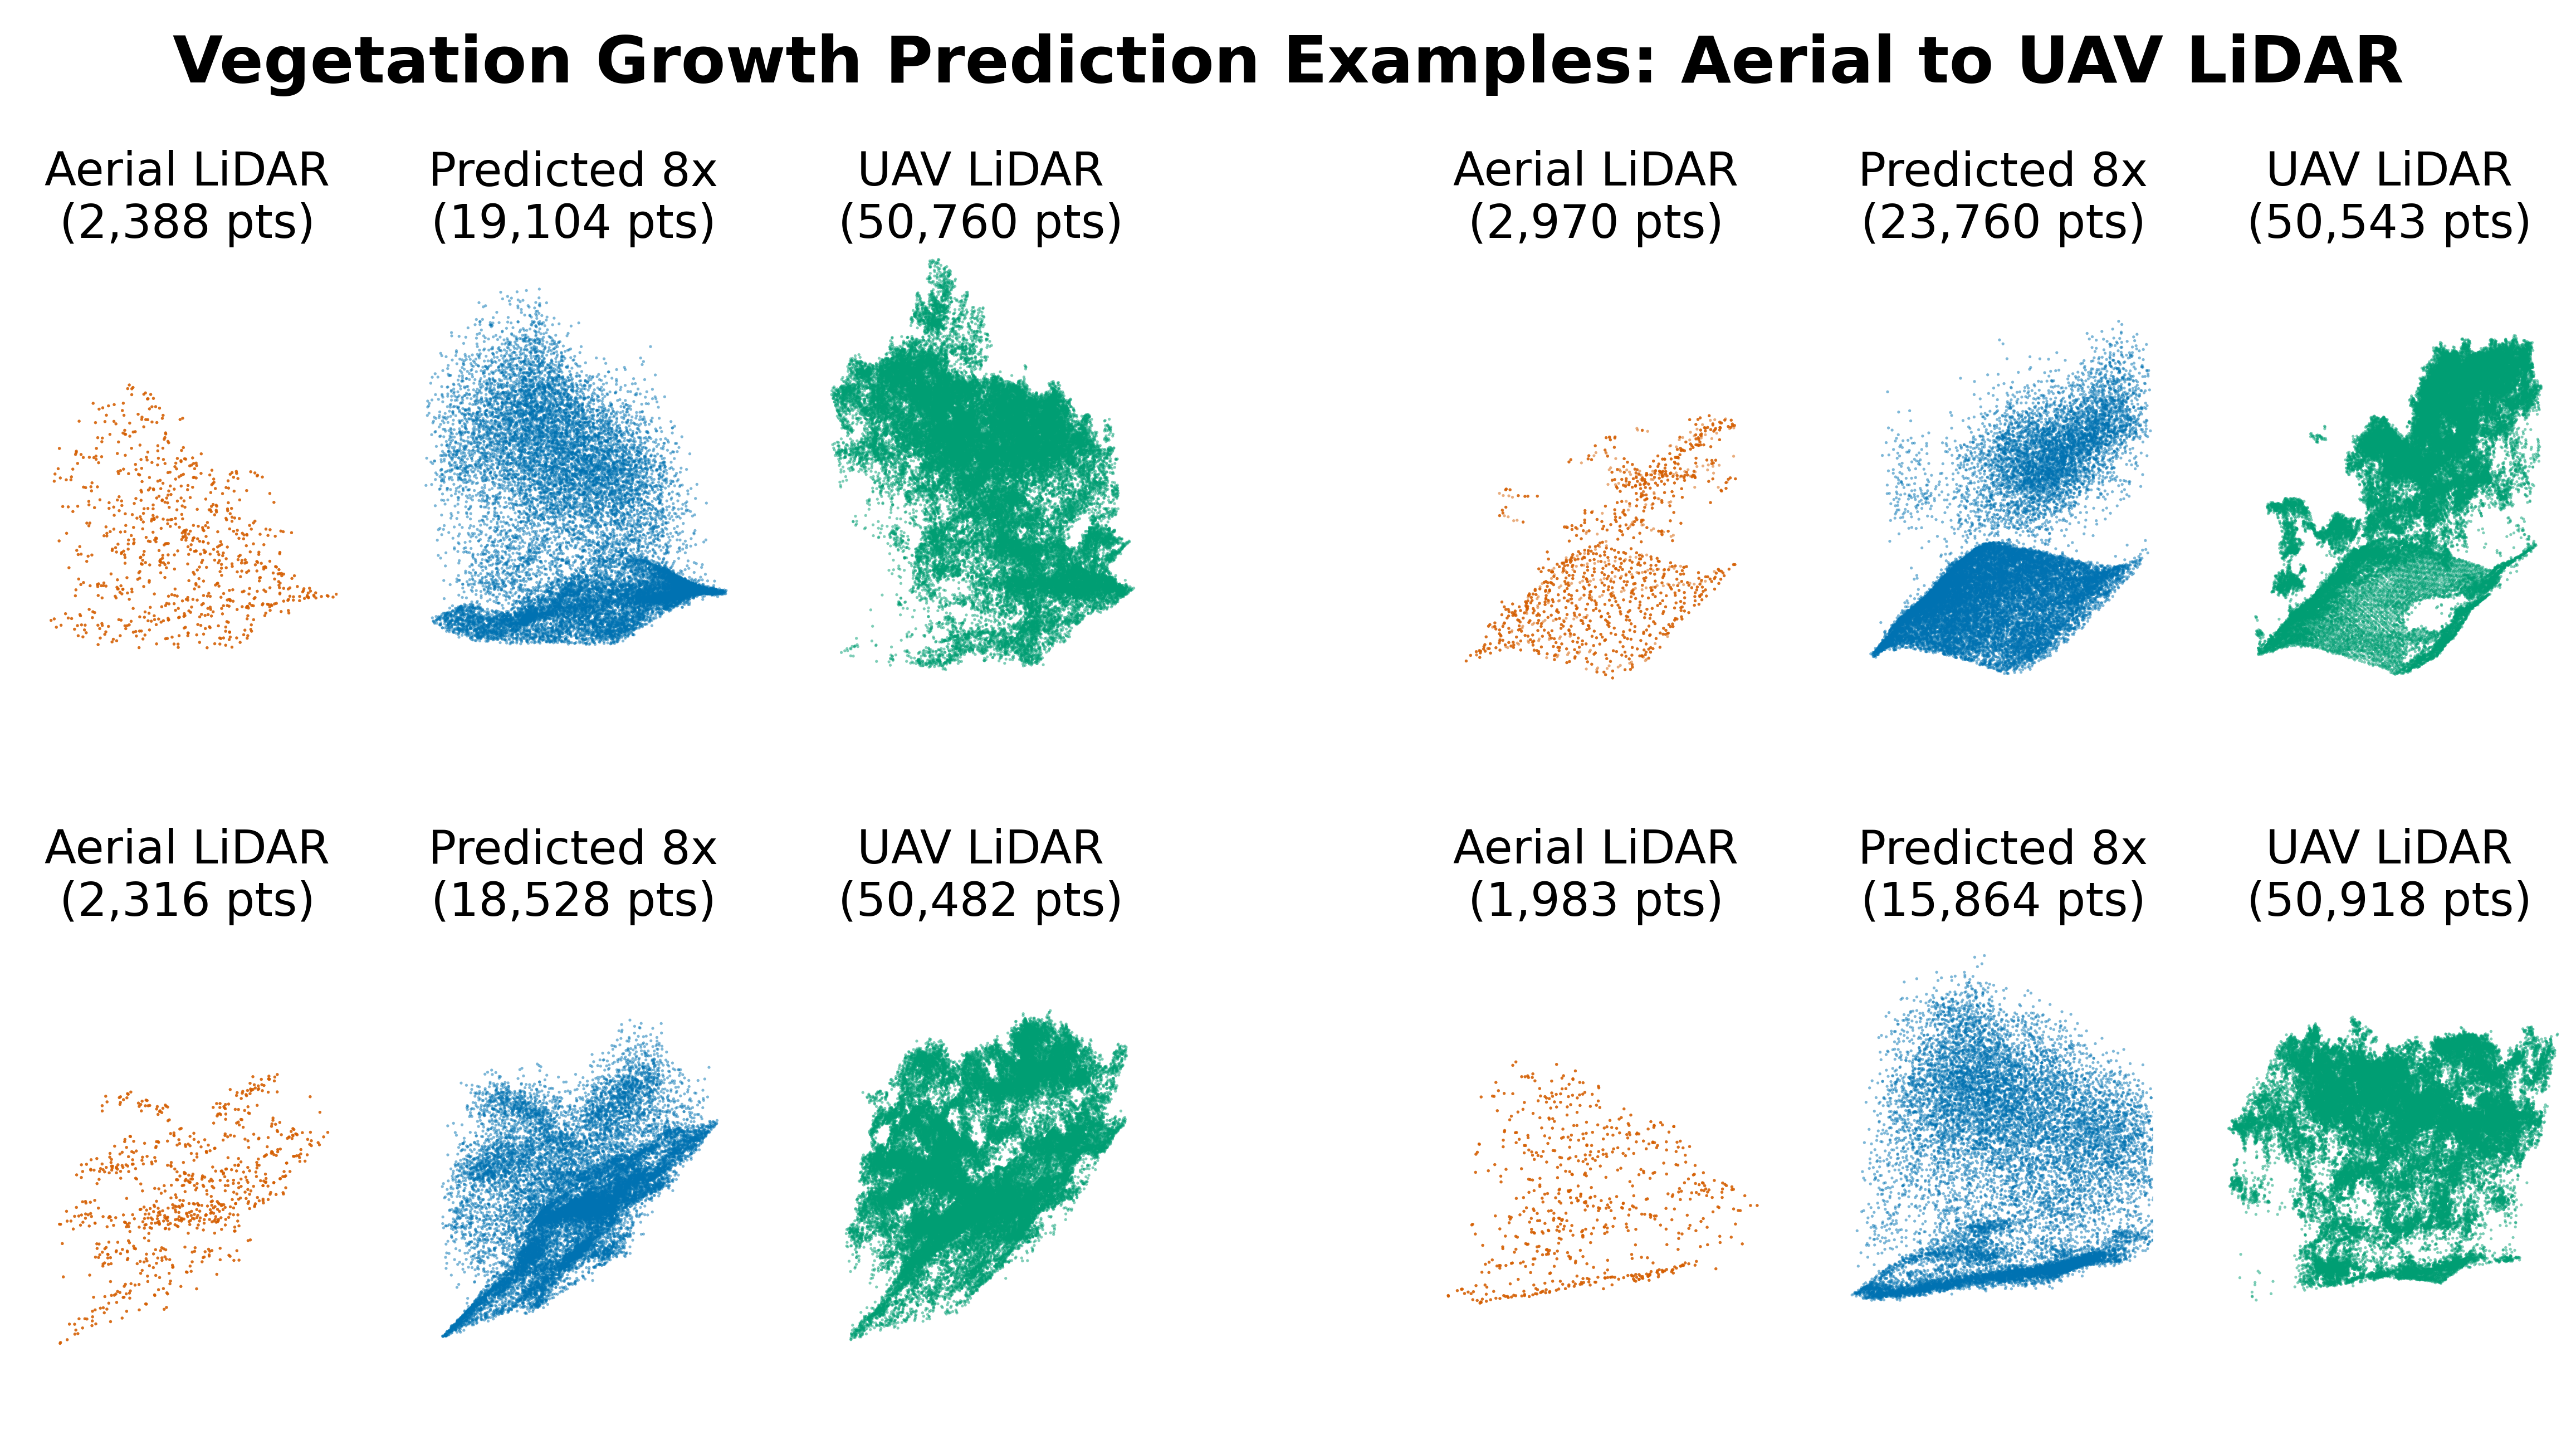
\includegraphics[width=0.98\linewidth]{figures/veg_growth2_8x.png}
    \end{adjustwidth}
    \caption{\hl{Second} %MDPI: 1. Commas are only used for numbers with five or more digits. We removed them in four-digit numbers in the figure. Please confirm. 2. Please confirm if explanation should be added for colors in the image.
vegetation growth example (experimental 8$\times$ visualization only; quantitative results use the 2$\times$ model) }
    \label{fig:appendix_growth2}
\end{figure}

\vspace{-11pt}

%%%%%%%%%%%%%%%%%%%%%%%%%%%%%%%%%%%%%%%%%%

\begin{figure}[H]
\begin{adjustwidth}{-\extralength}{0cm}
    \centering
    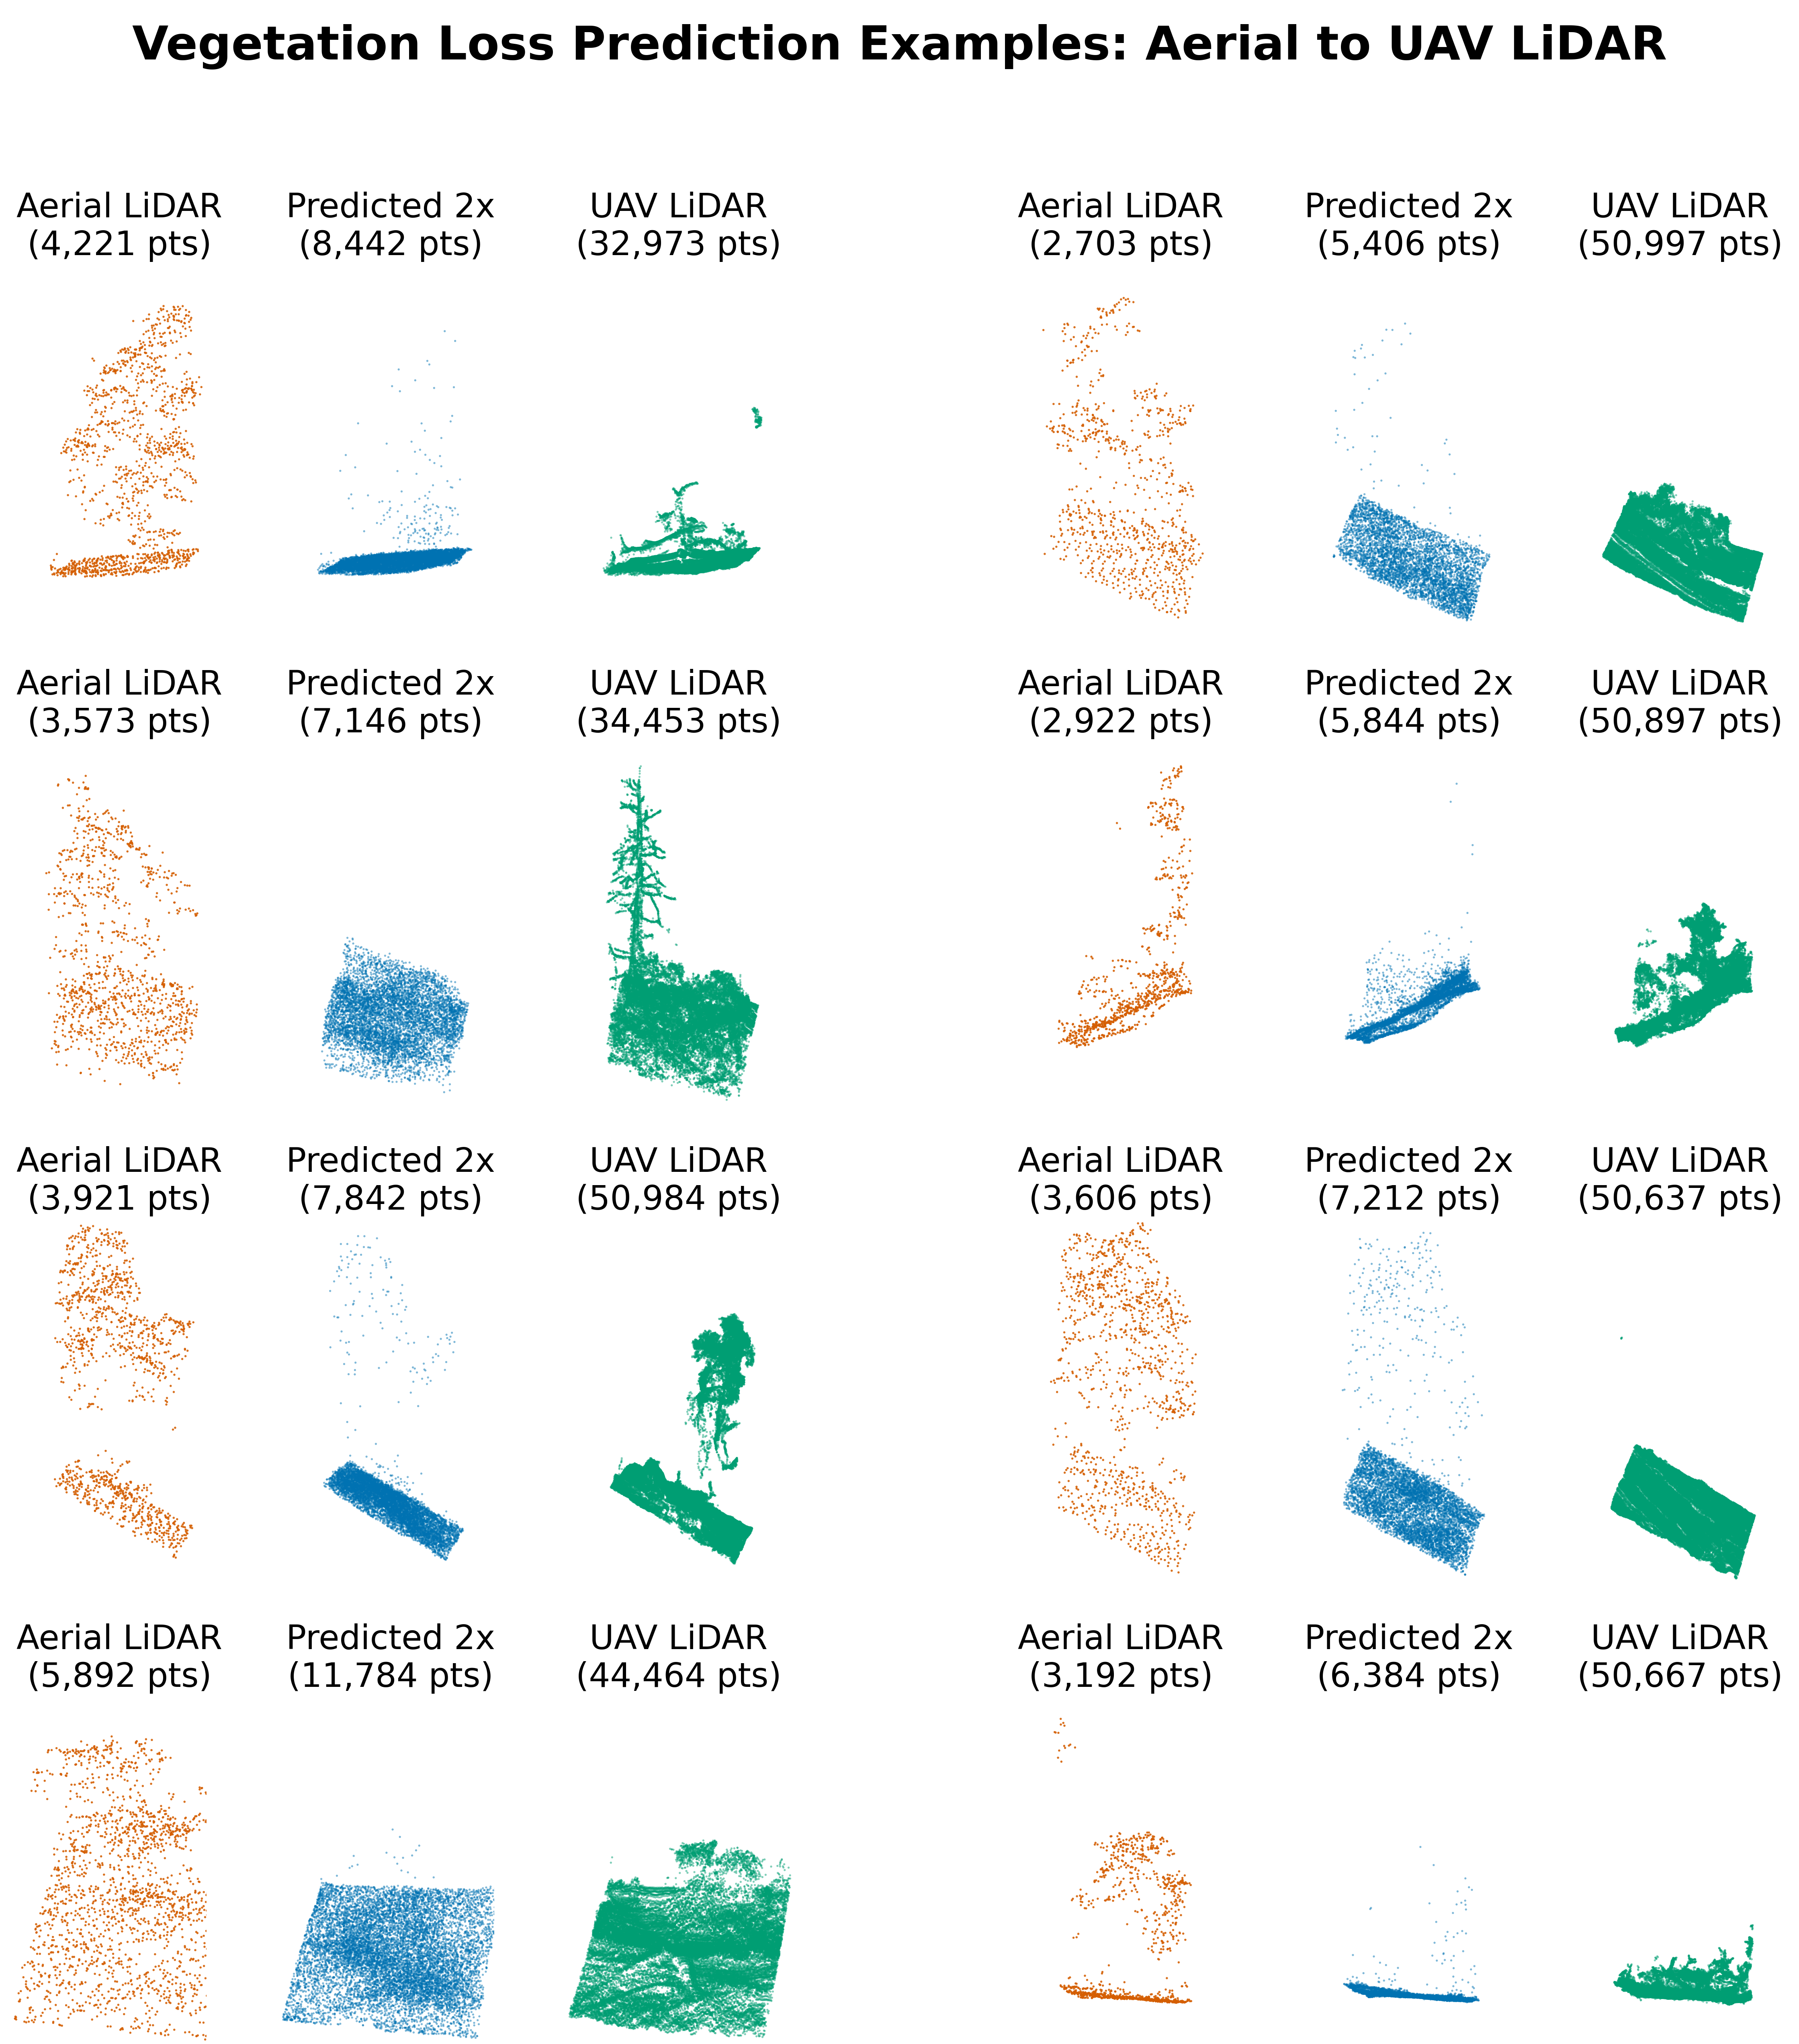
\includegraphics[width=0.98\linewidth]{figures/veg_loss_2x.png}
    \end{adjustwidth}
    \caption{\hl{Vegetation} %MDPI: 1. Commas are only used for numbers with five or more digits. We removed them in four-digit numbers in the figure. Please confirm. 2. Please confirm if explanation should be added for colors in the image. 3. To reduce the blank page, we made a sequel, please confirm. (MM: 1. Thank you, 2. Fine as-is, 3. Confirmed)
 loss example using the production 2$\times$ fusion model (configuration used for all quantitative evaluation). The model removes vegetation present in the outdated input LiDAR (left) to match the state shown in the recent UAV LiDAR reference (right), highlighting the value of multi-modal fusion for change detection.}
   \label{fig:appendix_loss}
\end{figure}

% %\isPreprints{}{% This command is only used for ``preprints''.
% \begin{adjustwidth}{-\extralength}{0cm}
% %} % If the paper is ``preprints'', please uncomment this parenthesis.
% %\printendnotes[custom] % Un-comment to print a list of endnotes

% \reftitle{References}

% % Please provide either the correct journal abbreviation (e.g. according to the “List of Title Word Abbreviations” http://www.issn.org/services/online-services/access-to-the-ltwa/) or the full name of the journal.
% % Citations and References in Supplementary files are permitted provided that they also appear in the reference list here.

% %=====================================
% % References, variant A: external bibliography
% %=====================================
% \bibliography{manuscript/references}

% \PublishersNote{}
% %\isPreprints{}{% This command is only used for ``preprints''.
% \end{adjustwidth}
% %} % If the paper is ``preprints'', please uncomment this parenthesis.

\begin{adjustwidth}{-\extralength}{0cm}
  % This code runs ONLY if it is NOT a preprint
  \reftitle{\highlighting{References} %MDPI: 1.Please do not change the reference format. Our production editor has done thoroughly layout work for the reference. Thanks for your cooperation.
}
  \begin{thebibliography}{999}

\bibitem[Martin-Ducup et~al.(2025)Martin-Ducup, Dupuy, Soma, Guerra-Hernandez,
  Marino, Fernandes, Just, Corbera, Toutchkov, Sorribas, Bock, Piboule,
  Pirotti, and Pimont]{martin-ducup_unlocking_2025}
Martin-Ducup, O.; Dupuy, J.L.; Soma, M.; Guerra-Hernandez, J.; Marino, E.;
  Fernandes, P.M.; Just, A.; Corbera, J.; Toutchkov, M.; Sorribas, C.;  et~al.
\newblock Unlocking the potential of Airborne {LiDAR} for direct assessment of
  fuel bulk density and load distributions for wildfire hazard mapping.
\newblock {\em Agric. For. Meteorol.} {\bf 2025}, {\em
  362}, \hl{110341}%MDPI: We removed the unnecessary information in this reference. Please confirm.
.
\newblock {\url{https://doi.org/10.1016/j.agrformet.2024.110341}}.

\bibitem[Merrick et~al.(2013)Merrick, Koprowski, and Wilcox]{Merrick2013Into3D}
Merrick, M.J.; Koprowski, J.L.; Wilcox, C.
\newblock Into the Third Dimension: Benefits of Incorporating {LiDAR} Data in
  Wildlife Habitat Models.
\newblock In \emph{Merging Science and Management in a Rapidly
  Changing World: Biodiversity and Management of the Madrean Archipelago III}; USDA Forest Service Proceedings RMRS-P-67; U.S. Department of Agriculture, Forest Service, Rocky Mountain Research Station: \hl{Fort Collins, CO, USA}%MDPI: We added the location of the publisher. Please confirm. (MM: confirmed)
, 2013; pp. 389--395.

\bibitem[Moudr{\`y} et~al.(2023)Moudr{\`y}, Cord, G{\'a}bor, Laurin,
  Bart{\'a}k, Gdulov{\'a}, Malavasi, Rocchini, Stere{\'n}czak, Pro{\v{s}}ek,
  et~al.]{moudry2023vegetation}
Moudr{\`y}, V.; Cord, A.F.; G{\'a}bor, L.; Laurin, G.V.; Bart{\'a}k, V.;
  Gdulov{\'a}, K.; Malavasi, M.; Rocchini, D.; Stere{\'n}czak, K.;
  Pro{\v{s}}ek, J.;  et~al.
\newblock Vegetation structure derived from airborne laser scanning to assess
  species distribution and habitat suitability: The way forward.
\newblock {\em Divers. Distrib.} {\bf 2023}, {\em 29},~39--50.

\bibitem[Agee(1996)]{agee_influence_1996}
Agee, J.K.
\newblock The Influence of Forest Structure on Fire Behavior. In Proceedings of the \hl{17th Annual Forest Vegetation Management Conference, Redding, CA, USA, 16–18 January} %MDPI: We added the conference title, location and date. Please confirm.(MM: confirmed)
 1996;
\newblock pp. 52--68.

\bibitem[Guo et~al.(2018)Guo, Coops, Gergel, Bater, Nielsen, Stadt, and
  Drever]{guo2018integrating}
Guo, X.; Coops, N.C.; Gergel, S.E.; Bater, C.W.; Nielsen, S.E.; Stadt, J.J.;
  Drever, M.
\newblock Integrating airborne lidar and satellite imagery to model habitat
  connectivity dynamics for spatial conservation prioritization.
\newblock {\em Landsc. Ecol.} {\bf 2018}, {\em 33},~491--511.

\bibitem[Mahata et~al.(2023)Mahata, Panda, Dash, Naik, Naik, and
  Palita]{mahata2023microclimate}
Mahata, A.; Panda, R.M.; Dash, P.; Naik, A.; Naik, A.K.; Palita, S.K.
\newblock Microclimate and vegetation structure significantly affect butterfly
  assemblages in a tropical dry forest.
\newblock {\em Climate} {\bf 2023}, {\em 11},~220.

\bibitem[Ustin and Middleton(2021)]{ustin2021current}
Ustin, S.L.; Middleton, E.M.
\newblock Current and near-term advances in Earth observation for ecological
  applications.
\newblock {\em Ecol. Processes} {\bf 2021}, {\em 10},~1.

\bibitem[Belov et~al.(2019)Belov, Belov, Gorodnichev, and
  Alkov]{belov2019capabilities}
Belov, M.; Belov, A.; Gorodnichev, V.; Alkov, S.
\newblock Capabilities analysis of lidar and passive optical methods for remote
  vegetation monitoring.
\newblock \emph{J. Phys. Conf. Ser.} \textbf{2019}, \emph{1399}, \hl{055024}%MDPI: We removed the unnecessary information in this reference. Please confirm. (MM: confirmed)
.

\bibitem[Guo et~al.(2020)Guo, Su, Hu, Guan, Jin, Zhang, Zhao, Xu, Wei, Kelly,
  et~al.]{guo2020lidar}
Guo, Q.; Su, Y.; Hu, T.; Guan, H.; Jin, S.; Zhang, J.; Zhao, X.; Xu, K.; Wei,
  D.; Kelly, M.;  et~al.
\newblock Lidar boosts 3D ecological observations and modelings: A review and
  perspective.
\newblock {\em IEEE Geosci. Remote Sens. Mag.} {\bf 2020}, {\em
  9},~232--257.

\bibitem[Wu et~al.(2016)Wu, Dye, Stoker, Vogel, Velasco, and
  Middleton]{wu2016evaluating}
Wu, Z.; Dye, D.; Stoker, J.; Vogel, J.; Velasco, M.; Middleton, B.
\newblock Evaluating LiDAR point densities for effective estimation of
  aboveground biomass.
\newblock {\em Int. J. Adv. Remote Sens. GIS} {\bf
  2016}, {\em 5},~1483--1499.

\bibitem[USGS(2019)]{usgs_what_2019}
USGS.
\newblock \emph{What Is {3DEP}?}; U.S. Geological Survey: \hl{Reston, VA, USA}%MDPI: We added the location of the publisher. Please confirm. (MM: confirmed)
, 2019.

\bibitem[USDA(2024)]{usda_naip_2024}
USDA.
\newblock \emph{National Agriculture Imagery Program---NAIP Hub Site}; \hl{USDA: Washington, DC, USA}%MDPI: We added the name of the publisher and its location. Please confirm. (MM: confirmed)
, 2024.

\bibitem[Wang et~al.(2025)Wang, Song, Schroeder, Woodcock, Pavelsky, Han, and
  Yao]{wang2025interpretable}
Wang, C.; Song, C.; Schroeder, T.A.; Woodcock, C.E.; Pavelsky, T.M.; Han, Q.;
  Yao, F.
\newblock Interpretable Multi-Sensor Fusion of Optical and SAR Data for
  GEDI-Based Canopy Height Mapping in Southeastern North Carolina.
\newblock {\em Remote Sens.} {\bf 2025}, {\em 17},~1536.

\bibitem[Rosen et~al.(2006)Rosen, Hensley, Wheeler, Sadowy, Miller, Shaffer,
  Muellerschoen, Jones, Zebker, and Madsen]{rosen2006uavsar}
Rosen, P.A.; Hensley, S.; Wheeler, K.; Sadowy, G.; Miller, T.; Shaffer, S.;
  Muellerschoen, R.; Jones, C.; Zebker, H.; Madsen, S.
\newblock UAVSAR: A new NASA airborne SAR system for science and technology
  research.
\newblock In Proceedings of the 2006 IEEE Conference on Radar, \hl{Verona, NY, USA, 24--27 April 2006}%MDPI: We added the location and date of the conference. Please confirm. The following highlights are the same. (MM: confirmed)
; IEEE: \hl{Piscataway, NJ, USA}%MDPI: We added the location of the publisher. Please confirm. The following highlights are the same. (MM: confirmed)
, 2006; p. 8.

\bibitem[Kellogg et~al.(2020)Kellogg, Hoffman, Standley, Shaffer, Rosen,
  Edelstein, Dunn, Baker, Barela, Shen, et~al.]{kellogg2020nasa}
Kellogg, K.; Hoffman, P.; Standley, S.; Shaffer, S.; Rosen, P.; Edelstein, W.;
  Dunn, C.; Baker, C.; Barela, P.; Shen, Y.;  et~al.
\newblock NASA-ISRO synthetic aperture radar (NISAR) mission.
\newblock In Proceedings of the 2020 IEEE Aerospace Conference, \hl{Big Sky, MT, USA, 7--14 March 2020}; IEEE: \hl{Piscataway, NJ, USA}, 2020;
  pp. 1--21.

\bibitem[Bahdanau et~al.(2014)Bahdanau, Cho, and Bengio]{bahdanau2014neural}
Bahdanau, D.; Cho, K.; Bengio, Y.
\newblock Neural machine translation by jointly learning to align and
  translate.
\newblock {\em arXiv} {\bf 2014}, arXiv:1409.0473.

\bibitem[Scheuring and Riedi(1994)]{scheuring1994application}
Scheuring, I.; Riedi, R.H.
\newblock Application of multifractals to the analysis of vegetation pattern.
\newblock {\em J. Veg. Sci.} {\bf 1994}, {\em 5},~489--496.

\bibitem[Yang et~al.(2015)Yang, Chen, Qian, Shen, and Wang]{yang2015extraction}
Yang, H.; Chen, W.; Qian, T.; Shen, D.; Wang, J.
\newblock The extraction of vegetation points from LiDAR using 3D fractal
  dimension analyses.
\newblock {\em Remote Sens.} {\bf 2015}, {\em 7},~10815--10831.

\bibitem[Vaswani et~al.(2017)Vaswani, Shazeer, Parmar, Uszkoreit, Jones, Gomez,
  Kaiser, and Polosukhin]{vaswani2017attention}
Vaswani, A.; Shazeer, N.; Parmar, N.; Uszkoreit, J.; Jones, L.; Gomez, A.N.;
  Kaiser, {\L}.; Polosukhin, I.
\newblock Attention is all you need.
\newblock In~{\em Advances in Neural Information Processing Systems}; \hl{Neural Information Processing Systems Foundation, Inc.: San Diego, CA, USA}%MDPI: We added the name of the publisher and its location. Please confirm. (MM: confirmed)
, 2017; Volume 30.

\bibitem[Dosovitskiy et~al.(2020)Dosovitskiy, Beyer, Kolesnikov, Weissenborn,
  Zhai, Unterthiner, Dehghani, Minderer, Heigold, Gelly,
  et~al.]{dosovitskiy2020image}
Dosovitskiy, A.; Beyer, L.; Kolesnikov, A.; Weissenborn, D.; Zhai, X.;
  Unterthiner, T.; Dehghani, M.; Minderer, M.; Heigold, G.; Gelly, S.;  et~al.
\newblock An image is worth 16 $\times$ 16 words: Transformers for image recognition at
  scale.
\newblock {\em arXiv} {\bf 2020}, arXiv:2010.11929.

\bibitem[Aleissaee et~al.(2023)Aleissaee, Kumar, Anwer, Khan, Cholakkal, Xia,
  and Khan]{aleissaee2023transformers}
Aleissaee, A.A.; Kumar, A.; Anwer, R.M.; Khan, S.; Cholakkal, H.; Xia, G.S.;
  Khan, F.S.
\newblock Transformers in remote sensing: A survey.
\newblock {\em Remote Sens.} {\bf 2023}, {\em 15},~1860.

\bibitem[Wilkes et~al.(2015)Wilkes, Jones, Suarez, Mellor, Woodgate,
  Soto-Berelov, Haywood, and Skidmore]{wilkes_mapping_2015}
Wilkes, P.; Jones, S.D.; Suarez, L.; Mellor, A.; Woodgate, W.; Soto-Berelov,
  M.; Haywood, A.; Skidmore, A.K.
\newblock Mapping Forest Canopy Height Across Large Areas by Upscaling {ALS}
  Estimates with Freely Available Satellite Data. \emph{\hl{Remote Sens.}%MDPI: We added the journal name. Please confirm. The same for the following highlights. (MM: confirmed)
} {\bf 2015},
\newblock {\em 7}, 12563--\hl{12587}%MDPI: We removed the unnecessary information for this reference. Please confirm.  (MM: confirmed)
.
\newblock {\url{https://doi.org/10.3390/rs70912563}}.

\bibitem[Wagner et~al.(2024)Wagner, Roberts, Ritz, Carter, Dalagnol, Favrichon,
  Hirye, Brandt, Ciais, and Saatchi]{wagner_sub-meter_2024}
Wagner, F.H.; Roberts, S.; Ritz, A.L.; Carter, G.; Dalagnol, R.; Favrichon, S.;
  Hirye, M.C.M.; Brandt, M.; Ciais, P.; Saatchi, S.
\newblock Sub-meter tree height mapping of California using aerial images and
  {LiDAR}-informed U-Net model. \emph{\hl{Remote Sens. Environ.}} {\bf 2024}, {\em 305}, 114099.
\newblock {\url{https://doi.org/10.1016/j.rse.2024.114099}}.

\bibitem[Shendryk(2022)]{shendryk2022fusing}
Shendryk, Y.
\newblock Fusing GEDI with earth observation data for large area aboveground
  biomass mapping.
\newblock {\em Int. J. Appl. Earth Obs. Geoinf.} {\bf 2022}, {\em 115},~103108.

\bibitem[Li et~al.(2023)Li, Zhu, Yao, Yue, Garc{\'\i}a-Fern{\'a}ndez, Lim, and
  Levers]{li2023large}
Li, Z.; Zhu, X.; Yao, S.; Yue, Y.; Garc{\'\i}a-Fern{\'a}ndez, {\'A}.F.; Lim,
  E.G.; Levers, A.
\newblock A large scale Digital Elevation Model super-resolution Transformer.
\newblock {\em Int. J. Appl. Earth Obs. Geoinf.} {\bf 2023}, {\em 124},~103496.

\bibitem[Taneja et~al.(2023)Taneja, Wallace, Hillman, Reinke, Hilton, Jones,
  and Hally]{taneja2023up}
Taneja, R.; Wallace, L.; Hillman, S.; Reinke, K.; Hilton, J.; Jones, S.; Hally,
  B.
\newblock Up-scaling fuel hazard metrics derived from terrestrial laser
  scanning using a machine learning model.
\newblock {\em Remote Sens.} {\bf 2023}, {\em 15},~1273.

\bibitem[Gazzea et~al.(2023)Gazzea, Solheim, and Arghandeh]{gazzea2023high}
Gazzea, M.; Solheim, A.; Arghandeh, R.
\newblock High-resolution mapping of forest structure from integrated SAR and
  optical images using an enhanced U-net method.
\newblock {\em Sci. Remote Sens.} {\bf 2023}, {\em 8},~100093.

\bibitem[Remijnse(2024)]{remijnse2024upsampling}
Remijnse, T.
\newblock Upsampling LiDAR Point Clouds of Forest Environments Using Deep Learning. \hl{Master's Thesis, Wageningen University and Research, Wageningen, The Netherlands}%MDPI: We added the level and the university and its location for the thesis. Please confirm. (MM: confirmed)
, 2024.

\bibitem[Yu et~al.(2018)Yu, Li, Fu, Cohen-Or, and Heng]{yu2018pu}
Yu, L.; Li, X.; Fu, C.W.; Cohen-Or, D.; Heng, P.A.
\newblock Pu-net: Point cloud upsampling network.
\newblock In Proceedings of the IEEE Conference on Computer
  Vision and Pattern Recognition, \hl{Salt Lake City, UT, USA, 18--23 June} 2018; pp. 2790--2799.

\bibitem[Qian et~al.(2021)Qian, Abualshour, Li, Thabet, and Ghanem]{qian2021pu}
Qian, G.; Abualshour, A.; Li, G.; Thabet, A.; Ghanem, B.
\newblock Pu-gcn: Point cloud upsampling using graph convolutional networks.
\newblock In~Proceedings of the IEEE/CVF Conference on
  Computer Vision and Pattern Recognition, \hl{Nashville, TN, USA, 20--25 June} 2021; \mbox{pp. 11683--11692}.

\bibitem[Qiu et~al.(2022)Qiu, Anwar, and Barnes]{qiu2022pu}
Qiu, S.; Anwar, S.; Barnes, N.
\newblock Pu-transformer: Point cloud upsampling transformer.
\newblock In Proceedings of the Asian Conference on Computer
  Vision, \hl{Macao, China, 4--8 December} 2022; pp. 2475--2493.

\bibitem[Zhang and Filin(2022)]{zhang2022deep}
Zhang, T.; Filin, S.
\newblock Deep-Learning-Based Point Cloud Upsampling of Natural Entities and
  Scenes.
\newblock {\em  Int. Arch. Photogramm. Remote Sens. Spat. Inf. Sci.} {\bf 2022}, {\em 43},~321--327.

\bibitem[Yan et~al.(2025)Yan, Cao, Yan, Zhu, and Wang]{yan2025remote}
Yan, W.; Cao, L.; Yan, P.; Zhu, C.; Wang, M.
\newblock Remote sensing image change detection based on swin transformer and
  cross-attention mechanism.
\newblock {\em Earth Sci. Inform.} {\bf 2025}, {\em 18},~106.

\bibitem[Ma et~al.(2022)Ma, Zhang, and Pun]{ma2022crossmodal}
Ma, X.; Zhang, X.; Pun, M.O.
\newblock A crossmodal multiscale fusion network for semantic segmentation of
  remote sensing data.
\newblock {\em IEEE J. Sel. Top. Appl. Earth Obs. Remote Sens.} {\bf 2022}, {\em 15},~3463--3474.

\bibitem[Qingyun and Zhaokui(2022)]{qingyun2022cross}
Qingyun, F.; Zhaokui, W.
\newblock Cross-modality attentive feature fusion for object detection in
  multispectral remote sensing imagery.
\newblock {\em Pattern Recognit.} {\bf 2022}, {\em 130},~108786.

\bibitem[Li et~al.(2024)Li, Xue, Zhao, Li, and Zhang]{li2024cross}
Li, K.; Xue, Y.; Zhao, J.; Li, H.; Zhang, S.
\newblock A cross-attention integrated shifted window transformer for remote
  sensing image scene recognition with limited data.
\newblock {\em J. Appl. Remote Sens.} {\bf 2024}, {\em
  18}, \hl{036506}%MDPI: We revised the page number. Please confirm. The following highlight is the same. (MM: confirmed)
.

\bibitem[Yu and Huang(2024)]{yu2024dmsca}
Yu, W.; Huang, F.
\newblock DMSCA: Deep multiscale cross-modal attention network for
  hyperspectral and light detection and ranging data fusion and joint
  classification.
\newblock {\em J. Appl. Remote Sens.} {\bf 2024}, {\em
  18}, \hl{036505}.

\bibitem[Li et~al.(2024)Li, Liu, Sun, and Zheng]{li2024multi}
Li, Z.; Liu, R.; Sun, L.; Zheng, Y.
\newblock Multi-Feature Cross Attention-Induced Transformer Network for
  Hyperspectral and LiDAR Data Classification.
\newblock {\em Remote Sens.} {\bf 2024}, {\em 16},~2775.

\bibitem[Yang et~al.(2024)Yang, Zhou, Wang, Tian, and Liew]{yang2024lidar}
Yang, J.X.; Zhou, J.; Wang, J.; Tian, H.; Liew, A.W.C.
\newblock LiDAR-guided cross-attention fusion for hyperspectral band selection
  and image classification.
\newblock {\em IEEE Trans. Geosci. Remote Sens.} {\bf 2024},
  {\em 62}, \hl{5515815}%MDPI: We revised the page number. Please confirm.
.

\bibitem[Zhu et~al.(2024)Zhu, Wang, Hou, and Yu]{zhu2024cams}
Zhu, W.; Wang, H.; Hou, H.; Yu, W.
\newblock CAMS: A Cross Attention Based Multi-Scale LiDAR-Camera Fusion
  Framework for 3D Object Detection.
\newblock In \emph{\hl{Advances in Guidance, Navigation and Control}%MDPI: We added the book title. Please confirm. (MM: confirmed)
, Proceedings of the International Conference on Guidance,
  Navigation and Control}; Springer: \hl{Berlin/Heidelberg, Germany}, 2024; pp. 533--542.

\bibitem[Yoo et~al.(2020)Yoo, Kim, Kim, and Choi]{yoo20203d}
Yoo, J.H.; Kim, Y.; Kim, J.; Choi, J.W.
\newblock 3d-cvf: Generating joint camera and lidar features using cross-view
  spatial feature fusion for 3d object detection.
\newblock In Proceedings of the Computer Vision---ECCV 2020: 16th European  Conference, Glasgow, UK, 23--28 August 2020; Proceedings, Part XXVII 16; Springer: \hl{Berlin/Heidelberg, Germany}, 2020; pp. 720--736.

\bibitem[Wu et~al.(2021)Wu, Miao, and Fu]{wu2021point}
Wu, H.; Miao, Y.; Fu, R.
\newblock Point cloud completion using multiscale feature fusion and
  cross-regional attention.
\newblock {\em Image Vis. Comput.} {\bf 2021}, {\em 111},~104193.

\bibitem[Zhao et~al.(2021)Zhao, Jiang, Jia, Torr, and Koltun]{zhao2021point}
Zhao, H.; Jiang, L.; Jia, J.; Torr, P.H.; Koltun, V.
\newblock Point transformer.
\newblock In Proceedings of the IEEE/CVF International
  Conference on Computer Vision, \hl{Montreal, QC, Canada, 10--17 October} 2021; pp. 16259--16268.

\bibitem[Dao et~al.(2022)Dao, Fu, Ermon, Rudra, and
  R{\'e}]{dao2022flashattention}
Dao, T.; Fu, D.; Ermon, S.; Rudra, A.; R{\'e}, C.
\newblock Flashattention: Fast and memory-efficient exact attention with
  io-awareness.
\newblock {\em Adv. Neural Inf. Process. Syst.} {\bf 2022},
  {\em 35},~16344--16359.

\bibitem[{USGS}(2016)]{usgs_usgs_2016}
{USGS}.
\newblock \emph{{USGS} 3DEP---{CA} {SanDiego} 2015 C17 1}; \hl{USGS: Reston, VA, USA}%MDPI: We formatted it as book and added the publisher and location. Please confirm. (MM: confirmed)
, 2016.
\bibitem[{U.S. Geological Survey, 3D Elevation
  Program}()]{us_geological_survey_3d_elevation_program_usgs_2023}
{U.S. Geological Survey, 3D Elevation Program}.
\newblock \emph{USGS 3DEP Lidar Point Cloud (COPC)};
\newblock Microsoft Planetary Computer, Redmond, WA, USA, 2023. Available online: \url{https://planetarycomputer.microsoft.com/dataset/usgs-3dep-lidar-copc}
.

\bibitem[Microsoft(2025)]{planetary_computer}
Microsoft.
\newblock \emph{Microsoft {Planetary} {Computer}}; \hl{Microsoft: Redmond, WA, USA}%MDPI: We added the publisher and its location. Please confirm. The same for the following highlights. (MM: confirmed)
, 2025.

\bibitem[{Alaska Satellite Facility}(2024)]{alaska_search}
{Alaska Satellite Facility}.
\newblock {\emph{ASF Search Python API}}; \hl{Alaska Satellite Facility: Fairbanks, AK, USA}, 2024.

\bibitem[Zhu et~al.(2024)Zhu, Fan, and Weng]{zhu2024advancements}
Zhu, Q.; Fan, L.; Weng, N.
\newblock Advancements in point cloud data augmentation for deep learning: A
  survey.
\newblock {\em Pattern Recognit.} {\bf 2024}, \emph{\hl{153}%MDPI: We added the volume number. Please confirm. (MM: confirmed)
}, 110532.

\bibitem[Shorten and Khoshgoftaar(2019)]{shorten2019survey}
Shorten, C.; Khoshgoftaar, T.M.
\newblock A survey on image data augmentation for deep learning.
\newblock {\em J. Big Data} {\bf 2019}, {\em 6}, \hl{60}%MDPI: We revised the page. Please confirm. (MM: confirmed)
.

\bibitem[Lee et~al.(2021)Lee, Lee, and Song]{lee2021vision}
Lee, S.H.; Lee, S.; Song, B.C.
\newblock Vision Transformer for Small-Size Datasets: {SPT + LSA}.
\newblock {\em arXiv} {\bf 2021}, arXiv:2112.13492.

\bibitem[Touvron et~al.(2021)Touvron, Cord, Sablayrolles, Synnaeve, and
  J{\'e}gou]{touvron2021going}
Touvron, H.; Cord, M.; Sablayrolles, A.; Synnaeve, G.; J{\'e}gou, H.
\newblock Going Deeper with Image Transformers.
\newblock In Proceedings of the IEEE/CVF International
  Conference on Computer Vision (ICCV), \hl{Montreal, QC, Canada, 10--17 October} 2021; pp. 32--42.

\bibitem[d'Ascoli et~al.(2021)d'Ascoli, Touvron, Leavitt, Morcos, Biroli, and
  Sagun]{dascoli2021convit}
d'Ascoli, S.; Touvron, H.; Leavitt, M.L.; Morcos, A.S.; Biroli, G.; Sagun, L.
\newblock ConViT: Improving Vision Transformers with Soft Convolutional
  Inductive Biases.
\newblock In Proceedings of the 38th International
  Conference on Machine Learning (ICML), \hl{Virtual, 18--24 July} 2021; Volume 139, pp. 2286--2296.

\bibitem[Defazio et~al.(2024)Defazio, Yang, Mehta, Mishchenko, Khaled, and
  Cutkosky]{defazio_road_2024}
Defazio, A.; Yang, X.A.; Mehta, H.; Mishchenko, K.; Khaled, A.; Cutkosky, A.
\newblock The Road Less Scheduled. \emph{\hl{arXiv} %MDPI: We added the journal name and removed the unnecessary informat. Please confirm. (MM: confirmed)
} \textbf{2024}.
  {\url{https://doi.org/10.48550/arXiv.2405.15682}}.

\bibitem[Wu et~al.(2021)Wu, Pan, Zhang, Wang, Liu, and
  Lin]{wu_density-aware_2021}
Wu, T.; Pan, L.; Zhang, J.; Wang, T.; Liu, Z.; Lin, D.
\newblock Density-Aware Chamfer Distance as a Comprehensive Metric for Point
  Cloud Completion. \emph{\hl{arXiv} %MDPI: We added the journal name and removed the unnecessary informat. Please confirm. (MM: confirmed)
}  \textbf{2021}.
  {\url{https://doi.org/10.48550/arXiv.2111.12702}}.

\bibitem[{Clay Foundation Team}(2024)]{clay_model_v1p5}
{Clay Foundation Team}.
\newblock Clay Foundation Model: An Open-Source AI Foundation Model for Earth
  Observation. Software Version 1.5 (Commit <hash>), Apache-2.0 License. 2024. Available online:
\newblock \url{https://github.com/Clay-foundation/model} (\hl{accessed on 20 November 2025}%MDPI: Please add the access date (format: Date Month Year), e.g., accessed on 1 January 2020. (MM: added)
).

\bibitem[Liu et~al.(2024)Liu, Feng, Wang, Wang, Liu, Zhao, Dengr, Ruan, Dai,
  Guo, et~al.]{liu2024deepseek}
Liu, A.; Feng, B.; Wang, B.; Wang, B.; Liu, B.; Zhao, C.; Dengr, C.; Ruan, C.;
  Dai, D.; Guo, D.;  et~al.
\newblock Deepseek-v2: A strong, economical, and efficient mixture-of-experts
  language model.
\newblock {\em arXiv} {\bf 2024}, arXiv:2405.04434.

\end{thebibliography}

  \PublishersNote{}
  \end{adjustwidth}

%%%%%%%%%%%%%%%%%%%%%%%%%%%%%%%%%%%%%%%%%%
%% Optional




\end{document}